\documentclass[11pt,a4paper,openany,twoside]{book}
% ---------------------------------------------------------------------------
% Preamble for the RSNA knee script. Compiled with Tectonic (XeTeX engine).
% ---------------------------------------------------------------------------
\usepackage{fontspec}                 % Latin Modern = the classic LaTeX look
\usepackage[english]{babel}
\usepackage[protrusion=true]{microtype}
\usepackage[a4paper,top=24mm,bottom=26mm,inner=27mm,outer=23mm,headheight=14pt]{geometry}
\usepackage{amsmath,amssymb}
\usepackage{graphicx}
\usepackage[dvipsnames,table]{xcolor}
\usepackage{tikz}
\usetikzlibrary{arrows.meta,positioning,calc,fit,backgrounds,shapes.geometric,shapes.misc,
  decorations.pathreplacing,patterns,matrix,shadows.blur}
\usepackage{pgfplots}
\pgfplotsset{compat=1.18}
\usepgfplotslibrary{groupplots,fillbetween,colormaps}
\usepackage[most]{tcolorbox}
\usepackage{booktabs,tabularx,array,multirow,makecell}
\usepackage{enumitem}
\usepackage{fancyhdr}
\usepackage{fontawesome5}
\usepackage[font=small,labelfont=bf,margin=4mm]{caption}
\usepackage{subcaption}
\usepackage{wrapfig}
\usepackage{float}
\usepackage{multicol}
\usepackage{pifont}
\usepackage{xspace}
\usepackage{xurl}
\usepackage[colorlinks=true,linkcolor=accentdark,urlcolor=accentdark,citecolor=accentdark]{hyperref}

\setlength{\parindent}{0pt}
\setlength{\emergencystretch}{2.5em}
\setlength{\parskip}{0.55em}
\linespread{1.06}
\setlist{itemsep=0.15em,topsep=0.3em}
\renewcommand{\arraystretch}{1.18}

% ---------------------------------------------------------------- colours
% Chart colours: first three slots of a colour-blind-checked palette.
\definecolor{us}{HTML}{2A78D6}        % our pipeline (blue)
\definecolor{them}{HTML}{EB6834}      % the winners (orange)
\definecolor{third}{HTML}{1BAF7A}     % a third series (aqua)
\definecolor{ink}{HTML}{1F1F1D}
\definecolor{muted}{HTML}{6B6A66}
\definecolor{grid}{HTML}{DDDCD8}
\definecolor{accent}{HTML}{2A78D6}
\definecolor{accentdark}{HTML}{1C5CAB}
% Box tints (light, so they print well; every box also carries an icon and a word)
\definecolor{keyfill}{HTML}{E8F1FC}  \definecolor{keyline}{HTML}{2A78D6}
\definecolor{whyfill}{HTML}{FFF4DC}  \definecolor{whyline}{HTML}{C98500}
\definecolor{wordfill}{HTML}{E6F6EF} \definecolor{wordline}{HTML}{14855C}
\definecolor{warnfill}{HTML}{FCE9E8} \definecolor{warnline}{HTML}{D03B3B}
\definecolor{numfill}{HTML}{F1F0EC}  \definecolor{numline}{HTML}{6B6A66}
\definecolor{tldrfill}{HTML}{F3EFFC} \definecolor{tldrline}{HTML}{6250D6}
% MRI-ish greys for drawings
\definecolor{bone}{HTML}{8C8C8C}
\definecolor{marrow}{HTML}{B5B5B5}
\definecolor{fluid}{HTML}{F5F5F5}
\definecolor{dark}{HTML}{202020}
\definecolor{softtissue}{HTML}{5E5E5E}

% ---------------------------------------------------------------- boxes
\tcbset{
  base/.style={enhanced, boxrule=0pt, leftrule=2.2mm, arc=1.2mm, outer arc=1.2mm,
    left=3mm, right=3mm, top=1.6mm, bottom=1.6mm, before skip=0.9em, after skip=0.9em,
    fonttitle=\bfseries\small, coltitle=ink, attach title to upper={\ \ }, parbox=false},
}
% Each box: colour + icon + word, so the meaning survives black-and-white printing.
\newtcolorbox{keyidea}[1][]{base, colback=keyfill, colframe=keyline,
  title={\textcolor{keyline}{\faLightbulb[regular]}\ Key idea#1}}
\newtcolorbox{why}[1][]{base, colback=whyfill, colframe=whyline,
  title={\textcolor{whyline}{\faQuestionCircle[regular]}\ Why?#1}}
\newtcolorbox{wordcheck}[1][]{base, colback=wordfill, colframe=wordline,
  title={\textcolor{wordline}{\faBookOpen}\ Word check#1}}
\newtcolorbox{watchout}[1][]{base, colback=warnfill, colframe=warnline,
  title={\textcolor{warnline}{\faExclamationTriangle}\ Watch out#1}}
\newtcolorbox{innumbers}[1][]{base, colback=numfill, colframe=numline,
  title={\textcolor{numline}{\faCalculator}\ In numbers#1}}
\newtcolorbox{example}[1][]{base, colback=white, colframe=numline, leftrule=0.6mm, boxrule=0.4pt,
  title={\textcolor{numline}{\faSearch}\ Example#1}}
\newtcolorbox{tldr}{enhanced, colback=tldrfill, colframe=tldrline, boxrule=0.6pt, arc=1.5mm,
  left=3.5mm, right=3.5mm, top=2mm, bottom=2mm, before skip=0.4em, after skip=1.1em,
  title={\faStopwatch\ \ In one minute}, fonttitle=\bfseries, coltitle=white, colbacktitle=tldrline}
\newtcolorbox{checkpoint}{enhanced, colback=white, colframe=tldrline, boxrule=0.6pt, arc=1.5mm,
  left=3.5mm, right=3.5mm, top=2mm, bottom=2mm, before skip=1.2em,
  title={\faFlagCheckered\ \ Checkpoint}, fonttitle=\bfseries, coltitle=white, colbacktitle=tldrline}

% Checklist and question items inside a checkpoint
\newcommand{\done}{\item[\textcolor{tldrline}{\faCheckSquare[regular]}]}
\newcommand{\quiz}{\item[\textcolor{tldrline}{\faQuestion}]}

% ---------------------------------------------------------------- small helpers
\newcommand{\term}[1]{\textbf{#1}}
\newcommand{\ca}{\ensuremath{\sim}}           % "about" sign                 % a new word, defined right here
\newcommand{\code}[1]{\texttt{\small #1}}
\newcommand{\finding}[1]{\textsf{#1}}
\newcommand{\us}{\textcolor{us}{\textbf{us}}\xspace}
\newcommand{\them}{\textcolor{them}{\textbf{winners}}\xspace}
\newcommand{\aucv}[1]{\textbf{#1}}
\newcommand{\up}{\textcolor{third}{\ding{115}}}    % small up-triangle
\newcommand{\down}{\textcolor{warnline}{\ding{116}}}
\newcommand{\cmark}{\textcolor{wordline}{\ding{51}}}
\newcommand{\xmark}{\textcolor{warnline}{\ding{55}}}
\newcommand{\figsrc}[1]{\par\vspace{-0.4em}{\scriptsize\textcolor{muted}{#1}}}

% ---------------------------------------------------------------- "where are we?" strip
% \whereami{k}: draws the pipeline and highlights stage k (0 = none).
\newcommand{\whereami}[1]{%
  \begin{center}
  \begin{tikzpicture}[x=1mm,y=1mm,
      st/.style={draw=grid, fill=white, rounded corners=1.2mm, minimum height=7mm, minimum width=21mm,
                 font=\scriptsize\sffamily, text=muted, inner sep=1pt, align=center},
      on/.style={draw=accent, fill=keyfill, text=ink, font=\scriptsize\sffamily\bfseries, line width=0.8pt},
      ar/.style={-{Stealth[length=1.6mm]}, draw=grid, line width=0.7pt}]
    \foreach \i/\t in {1/{\faDatabase\\Data}, 2/{\faFile\\Labels}, 3/{\faLayerGroup\\Image cache},
                       4/{\faBrain\\Model}, 5/{\faPaperPlane\\Submission}, 6/{\faTrophy\\Leaderboard}} {
      \ifnum\i=#1
        \node[st,on] (s\i) at ({(\i-1)*26},0) {\t};
      \else
        \node[st] (s\i) at ({(\i-1)*26},0) {\t};
      \fi
    }
    \foreach \i [evaluate=\i as \j using int(\i+1)] in {1,...,5} { \draw[ar] (s\i) -- (s\j); }
    \node[font=\scriptsize\itshape, text=muted, anchor=south west, inner sep=0pt] at ([yshift=1mm]s1.north west) {where are we?};
  \end{tikzpicture}
  \end{center}\vspace{-0.6em}}

% ---------------------------------------------------------------- chapter titles (classic look, less empty space)
\usepackage{titlesec}
\titleformat{\chapter}[display]{\normalfont\huge\bfseries}{\chaptertitlename\ \thechapter}{10pt}{\Huge}
\titlespacing*{\chapter}{0pt}{-12pt}{22pt}

% ---------------------------------------------------------------- headers
\pagestyle{fancy}
\fancyhf{}
\fancyhead[LE]{\small\textsc{\leftmark}}
\fancyhead[RO]{\small\textsc{\rightmark}}
\fancyfoot[C]{\small\thepage}
\renewcommand{\headrulewidth}{0.3pt}

% ---------------------------------------------------------------- pgfplots defaults
\pgfplotsset{
  every axis/.append style={font=\small, axis line style={draw=muted}, tick style={draw=muted},
    major grid style={draw=grid, line width=0.3pt}, label style={text=ink}, tick label style={text=ink},
    legend style={draw=none, fill=none, font=\footnotesize}, legend cell align=left},
  barus/.style={fill=us, draw=white, line width=0.6pt},
  barthem/.style={fill=them, draw=white, line width=0.6pt},
  barthird/.style={fill=third, draw=white, line width=0.6pt},
}

\newcommand{\nPool}{4,349}
\newcommand{\nGold}{58}
\newcommand{\nLang}{12}
\newcommand{\aucacl}{0.934}
\newcommand{\aucsyn}{0.711}
\newcommand{\auceff}{0.955}
\newcommand{\goldPosACL}{24}
\newcommand{\goldPosSyn}{27}
\newcommand{\synSilent}{84}
\newcommand{\goldMacro}{0.884}
\newcommand{\bootLo}{0.855}
\newcommand{\bootHi}{0.911}
\newcommand{\bootSD}{0.017}

% ---------------------------------------------------------------------------
% Schematic knee drawings, reused by several chapters.
% Both macros draw into the current tikzpicture in a 10 x 12 unit frame (scale them with the picture).
%   \kneesagittal : side view of a knee, front of the leg (anterior) on the LEFT, like the MRI images.
%   \kneecoronal  : front view of a RIGHT knee; the lateral side is on the viewer's LEFT.
% Overlays (lesions, boxes, labels) are drawn by each figure using the coordinates noted below.
% ---------------------------------------------------------------------------
\definecolor{kSoft}{HTML}{F5EDE8}     \definecolor{kSoftLine}{HTML}{D9C7BC}
\definecolor{kBone}{HTML}{EBDDC2}     \definecolor{kBoneLine}{HTML}{AE9B79}
\definecolor{kCart}{HTML}{8DB9E6}
\definecolor{kMen}{HTML}{3F6C9E}
\definecolor{kLig}{HTML}{C8553D}
\definecolor{kTendon}{HTML}{B79F78}
\definecolor{kFluid}{HTML}{CBE6F6}    \definecolor{kFluidLine}{HTML}{4E95CF}

% Sagittal landmarks: femoral condyle centre (5.5,6.75) r 1.95 | tibial plateau y = 4.55 (x 3.6-7.6)
% patella (2.85,7.55) | ACL (4.75,4.62)-(6.15,6.45) | anterior meniscus horn ~ (4.0,4.8), posterior horn ~ (7.0,4.8)
% suprapatellar recess (3.75,9.4) | Baker's cyst site (7.95,6.0)
\newcommand{\kneesagittal}{%
  \begin{scope}
    \clip (0,0) rectangle (10.5,12);
    \fill[kSoft, draw=kSoftLine, line width=0.6pt] plot[smooth cycle, tension=0.65] coordinates
      {(2.0,12.6) (1.75,10) (1.85,8.4) (2.15,7.0) (2.65,5.4) (3.0,4.0) (3.35,2.0) (3.45,-0.6) (7.65,-0.6)
       (7.9,2.0) (8.6,3.8) (9.05,5.6) (8.95,7.6) (8.55,9.8) (8.35,12.6)};
    % bone outlines first (thick), then fills on top = one outline around the union
    \begin{scope}[draw=kBoneLine, line width=1.4pt]
      \draw (4.5,12.6) -- (4.5,8.4) (6.5,8.4) -- (6.5,12.6);
      \draw (5.5,6.75) circle (1.95);
      \draw[rounded corners=6pt] (3.6,4.55) -- (7.6,4.55) -- (7.5,3.7) -- (6.6,2.9) -- (6.45,-0.6) -- (4.45,-0.6)
            -- (4.3,2.9) -- (3.75,3.45) -- cycle;
      \draw[rotate around={-8:(2.85,7.55)}] (2.85,7.55) ellipse (0.5 and 1.15);
    \end{scope}
    \fill[kBone] (4.5,12.6) -- (4.5,8.4) -- (6.5,8.4) -- (6.5,12.6) -- cycle;
    \fill[kBone] (4.5,8.6) -- (3.9,7.4) -- (7.1,7.4) -- (6.5,8.6) -- cycle;
    \fill[kBone] (5.5,6.75) circle (1.95);
    \fill[kBone, rounded corners=6pt] (3.6,4.55) -- (7.6,4.55) -- (7.5,3.7) -- (6.6,2.9) -- (6.45,-0.6) -- (4.45,-0.6)
          -- (4.3,2.9) -- (3.75,3.45) -- cycle;
    \fill[kBone, rotate around={-8:(2.85,7.55)}] (2.85,7.55) ellipse (0.5 and 1.15);
    % cartilage
    \draw[kCart, line width=2.2pt] (5.5,6.75) ++(165:1.84) arc (165:335:1.84);
    \draw[kCart, line width=2.0pt] (3.75,4.47) -- (7.45,4.47);
    \draw[kCart, line width=1.8pt, rotate around={-8:(2.85,7.55)}] (3.29,6.75) arc (-40:40:0.95);
    % tendons
    \draw[kTendon, line width=5pt, line cap=round] (3.1,12.6) -- (2.97,8.7);
    \draw[kTendon, line width=4pt, line cap=round] (2.72,6.45) -- (3.85,3.5);
    % joint fluid in the suprapatellar recess
    \fill[kFluid, draw=kFluidLine, line width=0.4pt] (3.78,9.4) ellipse (0.28 and 0.95);
    % menisci (anterior and posterior horn)
    \fill[kMen] (3.72,4.6) -- (4.6,4.6) -- (3.8,5.12) -- cycle;
    \fill[kMen] (6.45,4.6) -- (7.38,4.6) -- (7.28,5.2) -- cycle;
    % intercondylar notch (the gap between the condyles where the cruciates run), its roof line drawn as bone edge
    \fill[kSoft] (4.75,4.75) -- (6.95,4.75) -- (7.05,5.5) -- (6.5,6.7) -- (4.7,5.2) -- cycle;
    \draw[kBoneLine, line width=1pt] (4.7,5.2) -- (6.5,6.7);
    % cruciate ligaments
    \draw[kLig!55, line width=3pt, line cap=round] (6.85,4.35) .. controls (7.05,5.7) and (6.3,6.45) .. (5.25,6.2);
    \draw[kLig, line width=3.4pt, line cap=round] (4.75,4.62) -- (6.15,6.45);
  \end{scope}}

% Coronal landmarks (right knee, front view): lateral condyle (3.55,5.95) r 1.2, medial condyle (6.45,5.95) r 1.2
% tibial plateau y = 4.5 (x 2.3-7.7) | lateral meniscus ~ (2.75,4.8), medial meniscus ~ (7.25,4.8)
% MCL along x ~ 7.8 (y 2.2-6.9) | LCL (2.3,6.6)-(1.95,3.25) | notch (5.0,5.15)
\newcommand{\kneecoronal}{%
  \begin{scope}
    \clip (0,0) rectangle (10,12);
    \fill[kSoft, draw=kSoftLine, line width=0.6pt] plot[smooth cycle, tension=0.65] coordinates
      {(1.25,12.6) (1.0,9) (0.9,6.5) (1.2,4.5) (1.8,2.5) (2.3,-0.6) (7.7,-0.6) (8.2,2.5) (8.8,4.5) (9.1,6.5)
       (9.0,9) (8.75,12.6)};
    \begin{scope}[draw=kBoneLine, line width=1.4pt]
      \draw (4.0,12.6) -- (4.0,8.6) -- (2.45,6.6) (6.0,12.6) -- (6.0,8.6) -- (7.55,6.6);
      \draw (3.55,5.95) circle (1.2) (6.45,5.95) circle (1.2);
      \draw[rounded corners=6pt] (2.3,4.5) -- (7.7,4.5) -- (7.6,3.6) -- (6.2,2.6) -- (6.0,-0.6) -- (4.0,-0.6)
            -- (3.8,2.6) -- (2.4,3.6) -- cycle;
      \draw[rounded corners=4pt] (1.75,3.3) -- (2.55,3.3) -- (2.5,2.6) -- (2.35,-0.6) -- (1.95,-0.6) -- (1.85,2.6) -- cycle;
    \end{scope}
    \fill[kBone] (4.0,12.6) -- (4.0,8.6) -- (2.45,6.4) -- (7.55,6.4) -- (6.0,8.6) -- (6.0,12.6) -- cycle;
    \fill[kBone] (3.55,5.95) circle (1.2) (6.45,5.95) circle (1.2);
    \fill[kSoft] (5.0,5.05) ellipse (0.55 and 0.95);
    \fill[kBone, rounded corners=6pt] (2.3,4.5) -- (7.7,4.5) -- (7.6,3.6) -- (6.2,2.6) -- (6.0,-0.6) -- (4.0,-0.6)
          -- (3.8,2.6) -- (2.4,3.6) -- cycle;
    \fill[kBone] (4.65,4.45) -- (4.85,4.9) -- (5.15,4.9) -- (5.35,4.45) -- cycle;
    \fill[kBone, rounded corners=4pt] (1.75,3.3) -- (2.55,3.3) -- (2.5,2.6) -- (2.35,-0.6) -- (1.95,-0.6) -- (1.85,2.6) -- cycle;
    % cartilage
    \draw[kCart, line width=2.0pt] (3.55,5.95) ++(200:1.1) arc (200:330:1.1);
    \draw[kCart, line width=2.0pt] (6.45,5.95) ++(210:1.1) arc (210:340:1.1);
    \draw[kCart, line width=1.8pt] (2.55,4.43) -- (4.55,4.43) (5.45,4.43) -- (7.45,4.43);
    % menisci: wedges at the outer edges of the joint
    \fill[kMen] (2.25,4.58) -- (3.3,4.58) -- (2.35,5.15) -- cycle;
    \fill[kMen] (7.75,4.58) -- (6.7,4.58) -- (7.65,5.15) -- cycle;
    % collateral ligaments
    \draw[kLig, line width=3pt, line cap=round] plot[smooth] coordinates {(7.6,7.0) (7.86,4.7) (7.55,2.2)};
    \draw[kLig, line width=2.5pt, line cap=round] (2.3,6.6) -- (1.98,3.3);
    % cruciates in the notch
    \draw[kLig, line width=1.8pt, line cap=round] (4.8,4.55) -- (5.25,5.75);
    \draw[kLig!55, line width=1.8pt, line cap=round] (5.2,4.55) -- (4.78,5.8);
  \end{scope}}

% A small "label with leader line": \klabel{(point)}{(text position)}{anchor}{text}
\newcommand{\klabel}[4]{%
  \draw[ink!70, line width=0.4pt] #1 -- #2;
  \fill[ink!70] #1 circle (0.06);
  \node[anchor=#3, font=\scriptsize\sffamily, text=ink, inner sep=1.5pt, align=left] at #2 {#4};}


\title{Knee MRI, Labels and Leaderboards}
\begin{document}

\frontmatter
\begin{titlepage}
\thispagestyle{empty}
\vspace*{8mm}
{\large\scshape RSNA 2026 Knee Abnormality Detection\par}
\vspace{6mm}
{\fontsize{30}{36}\selectfont\bfseries Knee MRI, Labels\\[2mm] and Leaderboards\par}
\vspace{6mm}
{\Large A beginner's script: the data, everything we tried,\\ and how the winners did it\par}
\vspace{12mm}
\begin{center}
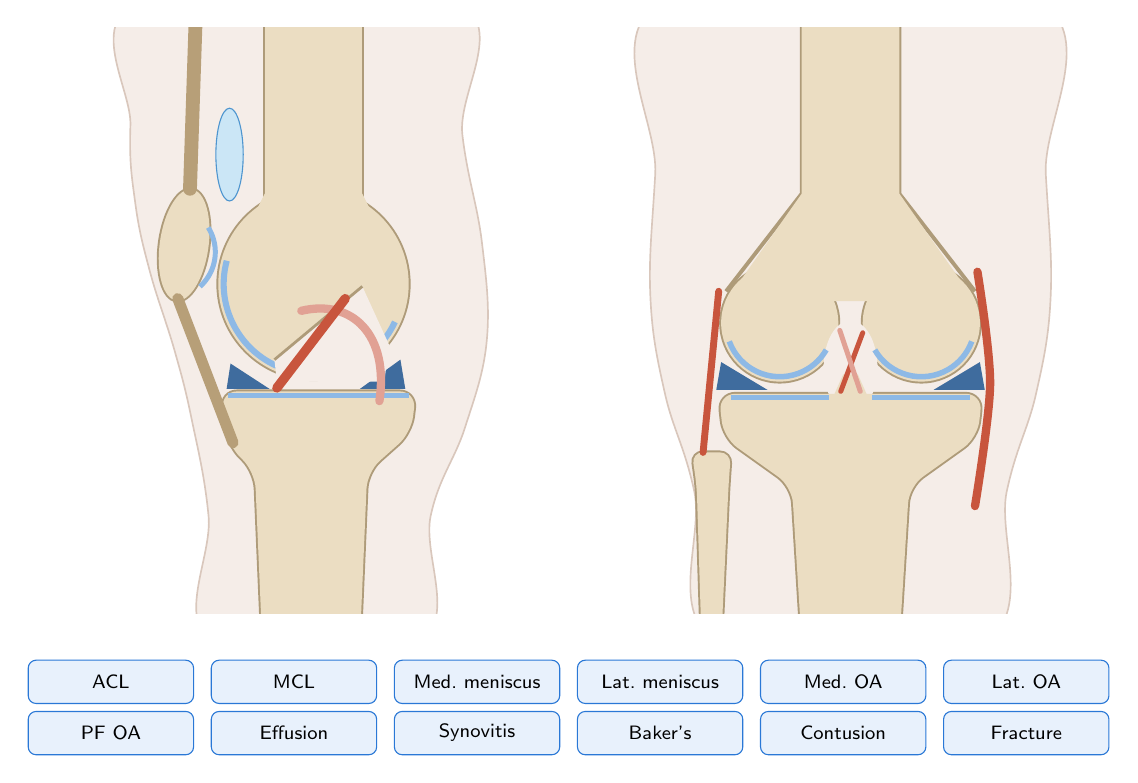
\begin{tikzpicture}[scale=0.62]
  \begin{scope}
    \kneesagittal
  \end{scope}
  \begin{scope}[xshift=11.5cm]
    \kneecoronal
  \end{scope}
  % twelve little finding tags
  \foreach \t [count=\i from 0] in {ACL,MCL,Med.\ meniscus,Lat.\ meniscus,Med.\ OA,Lat.\ OA,PF OA,Effusion,Synovitis,Baker's,Contusion,Fracture} {
    \pgfmathsetmacro{\col}{mod(\i,6)}
    \pgfmathsetmacro{\row}{int(\i/6)}
    \node[draw=accent, fill=keyfill, rounded corners=1mm, font=\scriptsize\sffamily, minimum width=21mm,
          minimum height=5.5mm] at ({\col*3.75+1.35}, {-1.4-\row*1.05}) {\t};
  }
\end{tikzpicture}
\end{center}
\vfill
{\large David Pilný\par}
{\normalsize written together with Claude (Anthropic)\par}
\vspace{2mm}
{\normalsize October 2026\par}
\vspace{6mm}
{\small\textcolor{muted}{Twelve findings, one knee MRI exam per row, 4,407 training exams and only 58 of them labelled by doctors.
This script explains how to turn that into a model, what we built, what scored what, and what the team that won did differently.}\par}
\end{titlepage}

{\hypersetup{linkcolor=ink}\tableofcontents}
\chapter*{How to read this script}
\addcontentsline{toc}{chapter}{How to read this script}
\markboth{How to read this script}{How to read this script}

This script is for someone who knows how to program but is new to medical imaging, to Kaggle competitions,
or to both. It follows one competition from start to finish: what the data looks like, which ideas we tried
and why, what each one scored, and what the team that finished first did.

\textbf{You do not need to read it in order.} Every chapter starts with a one-minute summary and ends with a
checkpoint. The pictures carry most of the story.

\section*{The boxes}

The text is broken up by coloured boxes. Each box has an icon and a word, so the meaning survives a
black-and-white printer.

\begin{tldr}
Three to five bullets at the start of every chapter. If you only read these, you get the whole story.
\end{tldr}
\begin{keyidea}
The one sentence to remember from a section.
\end{keyidea}
\begin{why}
The reason behind a choice. Read these when something feels arbitrary.
\end{why}
\begin{wordcheck}
A new word, explained in plain language the first time it appears. All of them are collected in the glossary
(Appendix~\ref{app:glossary}).
\end{wordcheck}
\begin{watchout}
A mistake that is easy to make, often one we made ourselves.
\end{watchout}
\begin{innumbers}
The figures that matter, in one place.
\end{innumbers}
\begin{example}
A small worked example, usually about one imaginary knee called \textbf{Study K}.
\end{example}
\begin{checkpoint}
\begin{itemize}
\done A short list of what you should now be able to explain.
\quiz Two or three questions to test yourself. The answers are in Appendix~\ref{app:answers}.
\end{itemize}
\end{checkpoint}

\section*{Three ways through}

\begin{center}
\begin{tikzpicture}[x=0.9mm,y=1mm,
  route/.style={draw=#1, line width=0.8pt, rounded corners=2mm, fill=white, minimum height=10mm,
                text width=34mm, align=center, font=\small},
  lab/.style={font=\small\bfseries, anchor=east}]
  \node[lab] at (-2,20) {\faStopwatch\ 15 minutes};
  \node[route=tldrline] at (24,20) {every \textbf{In one minute} box};
  \node[route=tldrline] at (70,20) {every \textbf{Checkpoint}};
  \node[route=tldrline] at (116,20) {Chapter~\ref{ch:usvsthem}: us vs.\ them};
  \node[lab] at (-2,6) {\faCoffee\ one hour};
  \node[route=keyline] at (24,6) {Part~I: the problem};
  \node[route=keyline] at (70,6) {Chapter~\ref{ch:experiments}: our experiments};
  \node[route=keyline] at (116,6) {Part~IV: the winners};
  \node[lab] at (-2,-8) {\faBook\ properly};
  \node[route=wordline, text width=118mm] at (70,-8) {front to back; Part~II explains the machine learning that Parts~III and IV use};
  \foreach \y in {20,6} {\draw[-{Stealth}, muted] (46.5,\y) -- (47.5,\y); \draw[-{Stealth}, muted] (92.5,\y) -- (93.5,\y);}
\end{tikzpicture}
\end{center}

\section*{The whole story on one page}

\begin{figure}[H]
\centering
\begin{tikzpicture}[x=1mm,y=1mm,
  stage/.style={draw=grid, fill=white, rounded corners=1.5mm, text width=29mm, minimum height=21mm,
                align=center, font=\footnotesize, inner sep=2pt},
  head/.style={font=\footnotesize\sffamily\bfseries, text=muted},
  ar/.style={-{Stealth[length=2mm]}, line width=0.8pt}]
  % column heads
  \foreach \x/\t in {0/{\faFile\ 1. Labels}, 33/{\faLayerGroup\ 2. Images in}, 66/{\faBrain\ 3. Model}, 99/{\faTrophy\ 4. Score}}
    \node[head] at (\x,17) {\t};
  % our lane
  \node[font=\small\bfseries, text=us, rotate=90] at (-21,0) {Us};
  \node[stage, draw=us, line width=0.8pt] (u1) at (0,0) {an open model reads the \textbf{report text}\\[1pt] agrees with doctors\\ \textbf{0.879} AUC};
  \node[stage, draw=us, line width=0.8pt] (u2) at (33,0) {3 series,\\ 24 slices each,\\ 256\,px, whole knee};
  \node[stage, draw=us, line width=0.8pt] (u3) at (66,0) {small CNNs\\ (EfficientNet-B0,\\ ConvNeXt-Nano)};
  \node[stage, draw=us, line width=0.8pt] (u4) at (99,0) {own model 0.918 public\\ best entry \textbf{0.927} private\\ rank 2,968 / 6,425};
  % winners lane
  \node[font=\small\bfseries, text=them, rotate=90] at (-21,-26) {Winners};
  \node[stage, draw=them, line width=0.8pt] (w1) at (0,-26) {AI agents read the \textbf{report and the images}\\[1pt] \textbf{0.94} AUC};
  \node[stage, draw=them, line width=0.8pt] (w2) at (33,-26) {5 series, all slices,\\ 384--512\,px,\\ + \textbf{anatomy boxes}};
  \node[stage, draw=them, line width=0.8pt] (w3) at (66,-26) {larger CNNs that\\ \textbf{look inside the boxes}};
  \node[stage, draw=them, line width=0.8pt] (w4) at (99,-26) {\textbf{0.960} private\\ rank 1\\ (one model: 0.954)};
  \foreach \a/\b in {u1/u2,u2/u3,u3/u4} \draw[ar, us] (\a) -- (\b);
  \foreach \a/\b in {w1/w2,w2/w3,w3/w4} \draw[ar, them] (\a) -- (\b);
  % the biggest gap
  \draw[decorate, decoration={brace, amplitude=2mm, mirror}, line width=0.7pt, ink]
     (-15,-38.5) -- (15,-38.5) node[midway, below=3mm, font=\footnotesize, text width=40mm, align=center]
     {\textbf{the biggest gap:} better labels};
\end{tikzpicture}
\caption{Our pipeline and the winners' pipeline, side by side. Both have the same four parts. The largest
difference is in the first one: how good the training labels are.}
\label{fig:story}
\end{figure}

\paragraph{The story in six sentences.}
\begin{enumerate}
\item The task: look at one knee MRI exam and give a probability for each of 12 problems (a torn ligament,
      a torn meniscus, fluid in the joint, \ldots).
\item Only 58 of the 4,407 training exams were labelled by doctors; the rest only have a free-text report.
\item So everybody first had to \textbf{turn reports into labels}, and then train an image model on those labels.
\item We did this with an open language model that read the reports, and trained small image models: 0.918 on
      our own, 0.927 on the final leaderboard with the help of a public notebook.
\item The winners let AI agents read the reports \emph{and look at the images}, and also asked them to draw boxes
      around the anatomy; their models scored 0.960.
\item Most of the gap comes from the labels, a smaller part from telling the model where to look.
\end{enumerate}


\mainmatter
\part{The problem}
\chapter{The competition in one chapter}
\label{ch:competition}

\begin{tldr}
\begin{itemize}
\item \textbf{Input:} one knee MRI exam (several 3D image stacks). \textbf{Output:} 12 probabilities, one per finding.
\item \textbf{Score:} ROC-AUC per finding, averaged over the 12 (rare findings count as much as common ones).
\item \textbf{Code competition:} you submit a notebook; Kaggle runs it offline on \ca 1,300 hidden exams, at most 9 hours.
\item \textbf{Two leaderboards:} public (30\,\% of the test exams, visible during the competition) and private
      (the other 70\,\%, revealed at the end, the one that counts).
\end{itemize}
\end{tldr}

\section{The task in one picture}

The organiser is the RSNA (Radiological Society of North America); the competition ran on Kaggle in
autumn 2026 with \$77{,}000 in prizes. The job: build a program that looks at a knee MRI exam and says, for
12 possible problems, how likely each one is.

\begin{figure}[H]
\centering
\begin{tikzpicture}[x=1mm,y=1mm]
  % a stack of slices for three series
  \foreach \s/\lab/\yy in {0/sagittal/12, 1/coronal/0, 2/axial/-12} {
    \foreach \k in {0,...,5} {
      \fill[dark!85, draw=white, line width=0.3pt] ({\k*1.4},{\yy+\k*1.1}) rectangle ++(9,7);
    }
    \node[font=\scriptsize\sffamily, anchor=east, text=muted] at (-1.5,\yy+5) {\lab};
  }
  \node[font=\footnotesize, align=center] at (9,-20) {one \textbf{exam} (``study'')\\ = several image stacks};
  % the model
  \node[draw=accent, fill=keyfill, rounded corners=2mm, minimum width=26mm, minimum height=20mm, align=center,
        font=\small] (m) at (48,4) {\faBrain\\[1mm] your model};
  \draw[-{Stealth[length=2.5mm]}, line width=1pt, muted] (20,4) -- (m.west);
  % twelve outputs
  \foreach \t/\p [count=\i from 0] in {ACL/0.93, MCL/0.08, Medial meniscus/0.21, Lateral meniscus/0.12,
      Medial OA/0.05, Lateral OA/0.03, PF OA/0.10, Effusion/0.81, Synovitis/0.30, Baker's/0.06,
      Contusion/0.88, Fracture/0.15} {
    \node[font=\scriptsize\sffamily, anchor=east] at (96,{24-\i*3.9}) {\t};
    \fill[grid] (97,{24-\i*3.9-1.2}) rectangle ++(30,2.4);
    \fill[us] (97,{24-\i*3.9-1.2}) rectangle ++({30*\p},2.4);
    \node[font=\scriptsize, anchor=west] at (128,{24-\i*3.9}) {\p};
  }
  \draw[-{Stealth[length=2.5mm]}, line width=1pt, muted] (m.east) -- (70,4);
  \node[font=\footnotesize, align=center] at (112,-26) {12 probabilities};
\end{tikzpicture}
\caption{The task. The example output is what a good model might say for \textbf{Study K}, an imaginary
footballer who twisted their knee: a torn ACL (0.93), fluid in the joint (0.81) and bruised bone (0.88).}
\label{fig:task}
\end{figure}

\begin{wordcheck}
\term{Study} (or exam): everything scanned in one visit, for one knee. \term{Series}: one 3D image stack inside
the study, taken in one direction with one setting (Chapter~\ref{ch:mri}). \term{Finding}: one of the 12 things
to detect.
\end{wordcheck}

\section{The twelve findings}

Chapter~\ref{ch:knee} explains each one with a drawing. For now, just the list:

\begin{center}
\small
\begin{tabularx}{\linewidth}{>{\bfseries}l >{\raggedright\arraybackslash}X >{\bfseries}l >{\raggedright\arraybackslash}X}
\toprule
\multicolumn{2}{l}{\textsf{Ligaments \& menisci (``soft parts that tear'')}} & \multicolumn{2}{l}{\textsf{Joint wear, fluid \& bone}} \\
\midrule
ACL & anterior cruciate ligament torn & Medial OA & cartilage worn away, inner side \\
MCL & medial collateral ligament torn & Lateral OA & cartilage worn away, outer side \\
Medial meniscus & inner shock absorber torn & PF OA & cartilage worn behind the kneecap \\
Lateral meniscus & outer shock absorber torn & Effusion & too much fluid in the joint \\
 & & Synovitis & inflamed joint lining \\
 & & Baker's & fluid cyst behind the knee \\
 & & Contusion & bruised bone \\
 & & Fracture & broken bone \\
\bottomrule
\end{tabularx}
\end{center}

A study can have none, one or many of them. Study~K has three. This is called a \term{multi-label}
problem: 12 independent yes/no questions about the same images.

\section{What ``code competition'' means}

In many Kaggle competitions you download the test data and upload a file of answers. Here you never see the
test images. You submit a \textbf{notebook} (a program), and Kaggle runs it on its own machine.

\begin{figure}[H]
\centering
\begin{tikzpicture}[x=0.88mm,y=1mm,
  box/.style={draw=grid, fill=white, rounded corners=1.5mm, align=center, font=\footnotesize, minimum height=14mm, inner sep=2mm},
  ar/.style={-{Stealth[length=2mm]}, line width=0.8pt, muted}]
  \node[box, text width=30mm] (you) at (0,0) {\faUser\\ you write and train\\ (with internet)};
  \node[box, text width=30mm] (nb) at (42,0) {\faFile\\ submission notebook\\ + attached model files};
  \node[box, text width=40mm, draw=accent, line width=0.8pt] (kg) at (92,0)
     {\faServer\\ Kaggle runs it on \ca 1,300 hidden exams\\ \textbf{no internet, at most 9 h}};
  \node[box, text width=24mm] (lb) at (135,0) {\faTrophy\\ score appears on the leaderboard};
  \draw[ar] (you) -- (nb); \draw[ar] (nb) -- (kg); \draw[ar] (kg) -- (lb);
  \node[font=\scriptsize, text=muted] at (92,-12) {scoring takes hours: ours took about 6\,h per submission};
\end{tikzpicture}
\caption{A code competition. Everything the notebook needs (model weights, extra Python packages) must be
attached in advance as Kaggle \emph{datasets}, because the scoring run is offline.}
\end{figure}

\begin{watchout}
A notebook that crashes on the hidden data gives no score, and you only find out hours later. That is why
every serious submission first writes a \textbf{safety-net} answer file (a constant guess) and then improves
on it study by study (Chapter~\ref{ch:submission}).
\end{watchout}

\section{The score: macro ROC-AUC}

For each finding Kaggle computes the \term{ROC-AUC}, then averages the 12 numbers. You will meet AUC properly
in Chapter~\ref{ch:auc}; for now one sentence is enough:

\begin{keyidea}
AUC = the chance that the model gives a randomly chosen \emph{sick} knee a higher score than a randomly chosen
\emph{healthy} knee. 0.5 is coin-flipping, 1.0 is perfect. Only the \emph{order} of the scores matters.
\end{keyidea}

Because the 12 AUCs are averaged with equal weight (a \term{macro} average), a rare finding like MCL tears
counts exactly as much as a common one like effusion.

\section{Two leaderboards}

\begin{figure}[H]
\centering
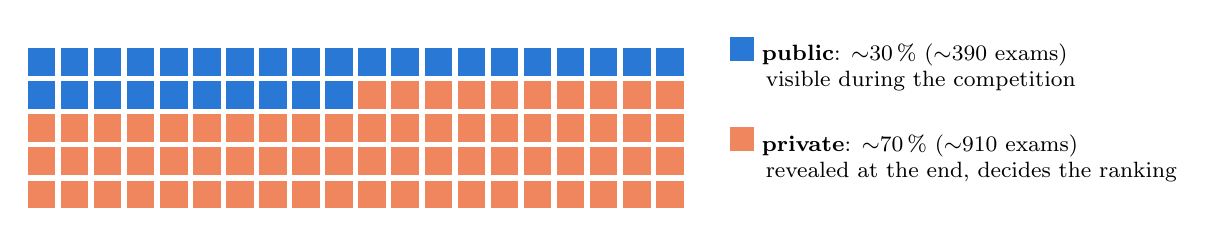
\begin{tikzpicture}[x=1mm,y=1mm]
  \foreach \i in {0,...,99} {
    \pgfmathsetmacro{\c}{mod(\i,20)}
    \pgfmathsetmacro{\r}{int(\i/20)}
    \ifnum\i<30
      \fill[us] ({\c*4.2},{-\r*4.2}) rectangle ++(3.5,3.5);
    \else
      \fill[them!80] ({\c*4.2},{-\r*4.2}) rectangle ++(3.5,3.5);
    \fi
  }
  \node[anchor=west, font=\footnotesize, align=left] at (88,1.5)
    {\textcolor{us}{\rule{3mm}{3mm}}\ \textbf{public}: \ca 30\,\% (\ca 390 exams)\\ \hspace*{4.5mm}visible during the competition};
  \node[anchor=west, font=\footnotesize, align=left] at (88,-10)
    {\textcolor{them!80}{\rule{3mm}{3mm}}\ \textbf{private}: \ca 70\,\% (\ca 910 exams)\\ \hspace*{4.5mm}revealed at the end, decides the ranking};
\end{tikzpicture}
\caption{The hidden test set is split once, at random. Each square is 1\,\% of the \ca 1,300 test exams.}
\end{figure}

\begin{why}\textbf{Why two leaderboards?}
If the score you see were the final score, you could submit many slightly different versions and keep the
luckiest one. This is called \term{overfitting the public leaderboard}. The private part stops it: a choice that
was only lucky on 390 exams does not stay lucky on the other 910.
\end{why}

\begin{innumbers}
With \ca 390 public exams the public score wobbles by about $\pm0.005$ from luck alone. Differences smaller than
that are noise. At the end you \textbf{select two submissions}; the better of the two on the private
leaderboard is your final result.
\end{innumbers}

\section{The efficiency track}

A second, smaller prize (\$7k / \$6k / \$5k) rewarded fast \emph{and} good submissions:
\[
\text{Efficiency} = \frac{\text{AUC}}{\text{Benchmark} - \text{maxAUC}} + \frac{\text{runtime in seconds}}{32{,}400}
\qquad\text{(lower is better)}
\]
The benchmark is below the best AUC, so the first term is negative: a higher AUC makes it more negative.
In practice this works out to roughly $-2.16\cdot\text{AUC} + \text{hours}/9$, so \textbf{one extra hour of
runtime costs about as much as 0.05 AUC}. A 4-minute notebook at 0.954 (the winners' single model) beats a
6-hour notebook at 0.96 easily.

\section{The calendar}

\begin{figure}[H]
\centering
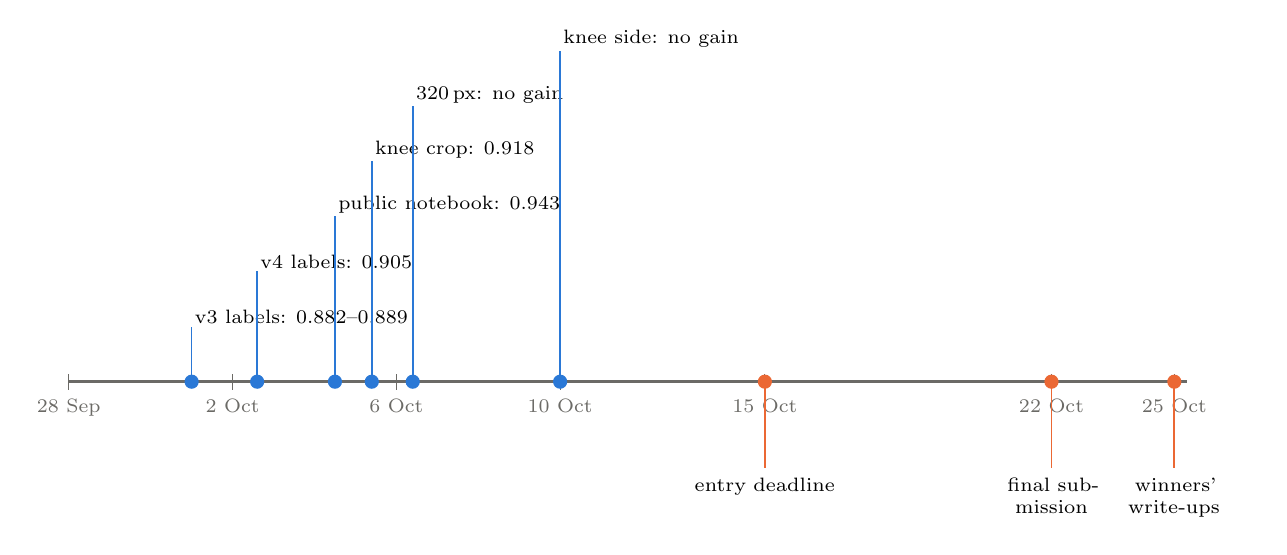
\begin{tikzpicture}[x=5.2mm,y=1mm]
  % day 0 = 28 Sep, day 27 = 25 Oct
  \draw[line width=1pt, muted] (0,0) -- (27.3,0);
  \foreach \d/\l in {0/28 Sep, 4/2 Oct, 8/6 Oct, 12/10 Oct, 17/15 Oct, 24/22 Oct, 27/25 Oct} {
    \draw[muted] (\d,-1) -- (\d,1);
    \node[font=\scriptsize, text=muted, below] at (\d,-1) {\l};
  }
  % our milestones (above)
  \foreach \d/\h/\t in {3/7/{v3 labels: 0.882--0.889}, 4.6/14/{v4 labels: 0.905}, 6.5/21/{public notebook: 0.943},
                        7.4/28/{knee crop: 0.918}, 8.4/35/{320\,px: no gain}, 12/42/{knee side: no gain}} {
    \draw[us, line width=0.6pt] (\d,0) -- (\d,\h);
    \fill[us] (\d,0) circle (0.9mm);
    \node[font=\scriptsize, anchor=south west, inner sep=1pt, fill=white] at (\d,\h) {\t};
  }
  % competition deadlines (below)
  \foreach \d/\t in {17/{entry deadline}, 24/{final submission}, 27/{winners' write-ups}} {
    \draw[them, line width=0.6pt] (\d,0) -- (\d,-11);
    \fill[them] (\d,0) circle (0.9mm);
    \node[font=\scriptsize, anchor=north, text width=19mm, align=center] at (\d,-11) {\t};
  }
\end{tikzpicture}
\caption{Our project in time (blue, public leaderboard scores) and the competition deadlines (orange). Our
active phase was the first two weeks of October.}
\end{figure}

\begin{checkpoint}
\begin{itemize}
\done I can say what goes in (one exam) and what comes out (12 probabilities).
\done I know why the public leaderboard is not the final score.
\quiz Q1.1: Why does a crashing notebook hurt more in a code competition than in a normal one?
\quiz Q1.2: The public score of your new version is 0.003 higher. Is it better?
\quiz Q1.3: In the efficiency track, is it worth adding a model that adds 0.01 AUC but one hour of runtime?
\end{itemize}
\end{checkpoint}

\chapter{The knee and its twelve findings}
\label{ch:knee}

\begin{tldr}
\begin{itemize}
\item The knee is where the thigh bone (femur) meets the shin bone (tibia); the kneecap (patella) glides in front.
\item Four kinds of parts can go wrong: \textbf{ropes} (ligaments), \textbf{cushions} (menisci),
      \textbf{surfaces} (cartilage), and \textbf{fluid and bone}.
\item The 12 findings are those parts, split into \textbf{medial} (inner) and \textbf{lateral} (outer) where it matters.
\item ``Positive'' means \textbf{severe enough}: a small effusion or a mild sprain counts as \emph{negative}.
\end{itemize}
\end{tldr}

\section{The parts of a knee}

\begin{wordcheck}
\term{Medial} = towards the middle of the body (the inner side of the knee). \term{Lateral} = away from the
middle (the outer side). \term{Anterior} = front, \term{posterior} = back. These words name the findings:
\emph{medial} meniscus, \emph{lateral} OA, \emph{anterior} cruciate ligament.
\end{wordcheck}

\paragraph{The parts in one line each.}
\begin{itemize}
\item \textbf{Bones:} femur on top, tibia below, patella in front, fibula on the outer side of the tibia.
\item \textbf{Cartilage:} a smooth layer (2--4\,mm) on the bone ends, so they glide.
\item \textbf{Menisci:} two C-shaped rubbery cushions between femur and tibia, one medial, one lateral.
\item \textbf{Ligaments:} ropes that hold the bones together. The two \textbf{cruciates} (ACL, PCL) cross inside
      the knee; the two \textbf{collaterals} (MCL inner, LCL outer) run along the sides.
\item \textbf{Synovium and joint fluid:} the joint is a sealed bag lined by the synovium, with a little lubricating
      fluid inside. The bag has a big pocket above the kneecap where extra fluid collects.
\end{itemize}

\begin{figure}[H]
\centering
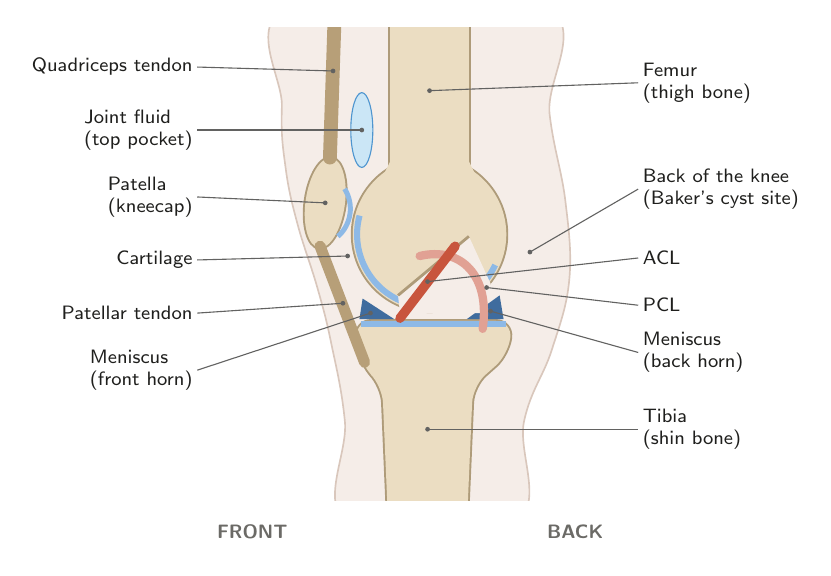
\begin{tikzpicture}[scale=0.5]
  \kneesagittal
  \klabel{(3.05,10.9)}{(-0.4,11.0)}{east}{Quadriceps tendon}
  \klabel{(3.78,9.4)}{(-0.4,9.4)}{east}{Joint fluid\\(top pocket)}
  \klabel{(2.85,7.55)}{(-0.4,7.7)}{east}{Patella\\(kneecap)}
  \klabel{(3.42,6.2)}{(-0.4,6.1)}{east}{Cartilage}
  \klabel{(3.3,5.0)}{(-0.4,4.75)}{east}{Patellar tendon}
  \klabel{(4.0,4.75)}{(-0.4,3.3)}{east}{Meniscus\\(front horn)}
  \klabel{(5.5,10.4)}{(10.8,10.6)}{west}{Femur\\(thigh bone)}
  \klabel{(8.05,6.3)}{(10.8,7.9)}{west}{Back of the knee\\(Baker's cyst site)}
  \klabel{(5.45,5.55)}{(10.8,6.15)}{west}{ACL}
  \klabel{(6.95,5.4)}{(10.8,4.95)}{west}{PCL}
  \klabel{(7.05,4.8)}{(10.8,3.75)}{west}{Meniscus\\(back horn)}
  \klabel{(5.45,1.8)}{(10.8,1.8)}{west}{Tibia\\(shin bone)}
  \node[font=\scriptsize\sffamily\bfseries, text=muted] at (1.0,-0.8) {FRONT};
  \node[font=\scriptsize\sffamily\bfseries, text=muted] at (9.2,-0.8) {BACK};
\end{tikzpicture}\hspace{4mm}
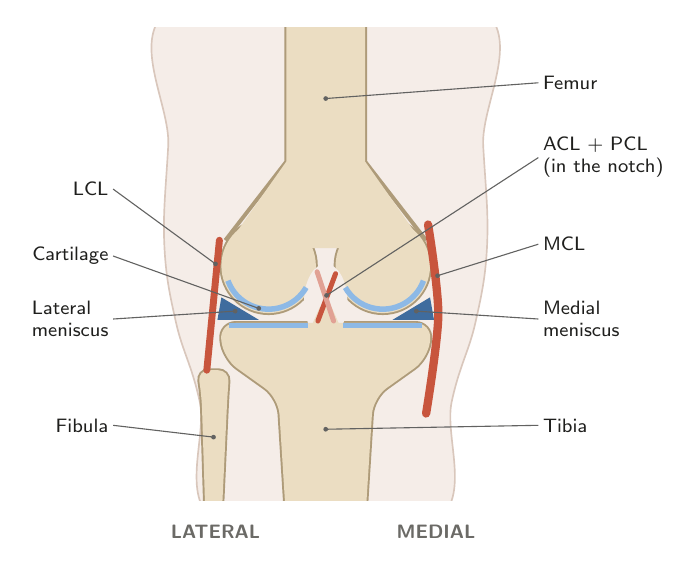
\begin{tikzpicture}[scale=0.5]
  \kneecoronal
  \klabel{(2.2,6.0)}{(-0.4,7.9)}{east}{LCL}
  \klabel{(3.3,4.87)}{(-0.4,6.2)}{east}{Cartilage}
  \klabel{(2.7,4.8)}{(-0.4,4.6)}{east}{Lateral\\meniscus}
  \klabel{(2.15,1.6)}{(-0.4,1.9)}{east}{Fibula}
  \klabel{(5.0,10.2)}{(10.4,10.6)}{west}{Femur}
  \klabel{(5.02,5.2)}{(10.4,8.7)}{west}{ACL + PCL\\(in the notch)}
  \klabel{(7.84,5.7)}{(10.4,6.5)}{west}{MCL}
  \klabel{(7.3,4.8)}{(10.4,4.6)}{west}{Medial\\meniscus}
  \klabel{(5.0,1.8)}{(10.4,1.9)}{west}{Tibia}
  \node[font=\scriptsize\sffamily\bfseries, text=muted] at (2.2,-0.8) {LATERAL};
  \node[font=\scriptsize\sffamily\bfseries, text=muted] at (7.8,-0.8) {MEDIAL};
\end{tikzpicture}
\caption{Left: a knee seen from the side (front of the leg on the left, as in the MRI images later). Right: a
right knee seen from the front. Blue wedges = menisci, light blue = cartilage, red = ligaments.}
\label{fig:anatomy}
\end{figure}

\section{Three compartments}

Doctors split the knee into three areas where two cartilage surfaces touch. Three of our findings are
``osteoarthritis in compartment X''.

\begin{figure}[H]
\centering
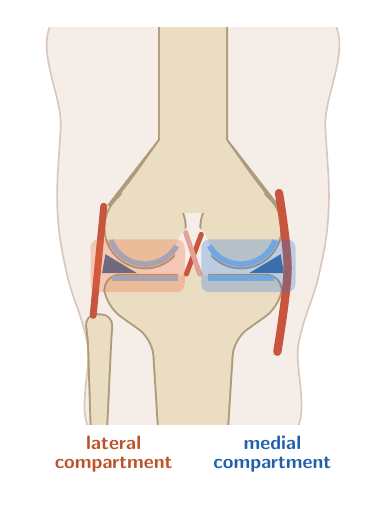
\begin{tikzpicture}[scale=0.42]
  \kneecoronal
  \fill[them, opacity=0.28, rounded corners=3pt] (1.9,4.0) rectangle (4.75,5.6);
  \fill[us, opacity=0.28, rounded corners=3pt] (5.25,4.0) rectangle (8.1,5.6);
  \node[font=\scriptsize\sffamily\bfseries, text=them!80!black, align=center] at (2.6,-0.9) {lateral\\[-1pt]compartment};
  \node[font=\scriptsize\sffamily\bfseries, text=us!80!black, align=center] at (7.4,-0.9) {medial\\[-1pt]compartment};
\end{tikzpicture}\hspace{10mm}
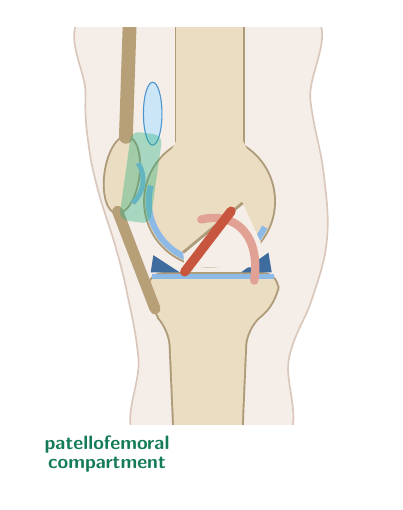
\begin{tikzpicture}[scale=0.42]
  \kneesagittal
  \fill[third, opacity=0.35, rotate around={-8:(2.85,7.55)}, rounded corners=3pt] (2.95,6.2) rectangle (3.9,8.9);
  \node[font=\scriptsize\sffamily\bfseries, text=third!70!black, align=center] at (2.4,-0.9) {patellofemoral\\[-1pt]compartment};
\end{tikzpicture}
\caption{\textbf{Medial OA} and \textbf{Lateral OA} are about the two tibiofemoral compartments (femur on tibia,
left). \textbf{PF OA} is about the patellofemoral compartment, where the kneecap glides on the femur (right).}
\label{fig:compartments}
\end{figure}

\section{The twelve findings, one card each}

Every card says what the finding is, when it counts as \textbf{positive} in this competition, and where it is
easiest to see (the planes are explained in Chapter~\ref{ch:mri}).

\newcommand{\findingcard}[5]{%
  \begin{tcolorbox}[enhanced, colback=white, colframe=grid, boxrule=0.5pt, arc=1.2mm,
     title={#1}, fonttitle=\bfseries\small, coltitle=ink, colbacktitle=keyfill,
     left=2mm, right=2mm, top=1mm, bottom=1mm, fontupper=\footnotesize]
  #2\par\smallskip
  \textcolor{wordline}{\faCheckCircle}\ \textbf{Positive if:} #3\par
  \textcolor{muted}{\faTimesCircle}\ \textbf{Negative:} #4\par
  \textcolor{accent}{\faEye}\ \textbf{Best seen:} #5
  \end{tcolorbox}}

\begin{tcbraster}[raster columns=2, raster equal height=rows, raster column skip=3mm, raster row skip=2.5mm]
\findingcard{ACL (anterior cruciate ligament)}
  {The rope in the middle of the knee that stops the shin bone sliding forward. Torn by twisting, typical in football and skiing.}
  {high-grade partial or complete tear (more than half the fibres).}
  {sprain, low-grade partial tear, signal change only.}
  {sagittal images.}
\findingcard{MCL (medial collateral ligament)}
  {The rope on the inner side. Torn when the knee is hit from the outside.}
  {acute high-grade or complete tear.}
  {low-grade sprain, old scarring.}
  {coronal images.}
\findingcard{Medial meniscus}
  {The inner cushion. Tears from twisting, or from wear in older knees.}
  {a tear reaching the meniscus surface (seen on $\geq$2 images), or a deformed meniscus.}
  {degeneration inside the meniscus that does not reach the surface.}
  {sagittal and coronal.}
\findingcard{Lateral meniscus}
  {The outer cushion. Same as the medial one, on the other side.}
  {same rule as the medial meniscus.}
  {same rule.}
  {sagittal and coronal.}
\findingcard{Medial OA (osteoarthritis)}
  {Cartilage worn away between femur and tibia on the inner side. The most common place for knee arthritis.}
  {an area of about 1\,cm or more where more than half of the cartilage thickness is lost.}
  {softening, thin fissures, small defects.}
  {coronal and sagittal.}
\findingcard{Lateral OA}
  {The same wear on the outer side.}
  {same rule, lateral compartment.}
  {same rule.}
  {coronal and sagittal.}
\findingcard{PF OA (patellofemoral)}
  {Cartilage worn between the kneecap and the groove of the femur.}
  {same rule, patellofemoral compartment.}
  {same rule.}
  {axial and sagittal.}
\findingcard{Effusion}
  {Too much fluid in the joint bag. A sign that something inside is irritated or injured.}
  {moderate or large amount.}
  {trace, small or ``physiological'' fluid.}
  {sagittal (pocket above the kneecap) and axial.}
\findingcard{Synovitis}
  {The lining of the joint is thickened and inflamed. Hard to see without contrast dye; reports often do not mention it.}
  {thickened, inflamed synovium.}
  {normal lining; fluid alone is not synovitis.}
  {axial and sagittal.}
\findingcard{Baker's cyst}
  {A fluid sac behind the knee, a bulge of the joint bag between two muscles.}
  {moderate or large cyst.}
  {small or tiny cyst.}
  {axial and sagittal.}
\findingcard{Contusion (bone bruise)}
  {Bleeding and swelling inside the bone after an impact. Bright on fat-suppressed images. Classic companion of an ACL tear.}
  {impact bone-marrow edema without a fracture line.}
  {edema from wear or overload.}
  {fat-suppressed fluid-sensitive images, any plane.}
\findingcard{Fracture}
  {A broken bone.}
  {an acute fracture line or break in the outer bone layer (cortex).}
  {old healed fractures.}
  {a line on T1 or PD images, with edema around it on fat-suppressed images.}
\end{tcbraster}

\section{``Positive'' means ``past a threshold''}

The doctors who made the reference labels used strict rules: a finding only counts if it is severe enough,
and a borderline case counts as \textbf{negative}. This matters a lot, because a radiology report mentions
small things too (``small effusion'', ``grade 1 sprain'').

\begin{figure}[H]
\centering
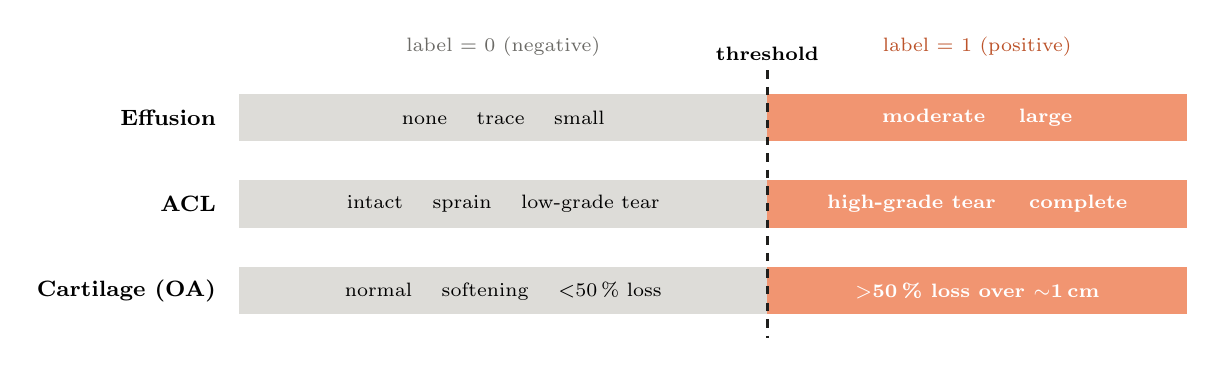
\begin{tikzpicture}[x=0.86mm,y=1mm]
  \foreach \y/\name/\neg/\pos in {0/Effusion/{none \quad trace \quad small}/{moderate \quad large},
                                 -11/ACL/{intact \quad sprain \quad low-grade tear}/{high-grade tear \quad complete},
                                 -22/Cartilage (OA)/{normal \quad softening \quad $<$50\,\% loss}/{$>$50\,\% loss over \ca 1\,cm}} {
    \node[anchor=east, font=\footnotesize\bfseries] at (-2,\y) {\name};
    \fill[grid] (0,\y-3) rectangle (78,\y+3);
    \fill[them!70] (78,\y-3) rectangle (140,\y+3);
    \node[font=\scriptsize] at (39,\y) {\neg};
    \node[font=\scriptsize, text=white] at (109,\y) {\textbf{\pos}};
  }
  \draw[ink, line width=1pt, dashed] (78,6) -- (78,-28);
  \node[font=\scriptsize\bfseries, anchor=south] at (78,6) {threshold};
  \node[font=\scriptsize, text=muted] at (39,9) {label = 0 (negative)};
  \node[font=\scriptsize, text=them!80!black] at (109,9) {label = 1 (positive)};
\end{tikzpicture}
\caption{Severity scales. Everything left of the dashed line is a \emph{negative} in this competition, even
though a report may describe it as a finding. Borderline cases also go to the left.}
\label{fig:thresholds}
\end{figure}

\begin{watchout}
Our first labeller (Chapter~\ref{ch:labels}) used the opposite rule, ``any grade counts''. That one sentence cost
us about 0.07 in label quality. \textbf{Read the organisers' definitions before you label anything.}
\end{watchout}

\section{What it looks like on real images}

\begin{figure}[H]
\centering
\begin{subfigure}[t]{0.31\linewidth}\centering
  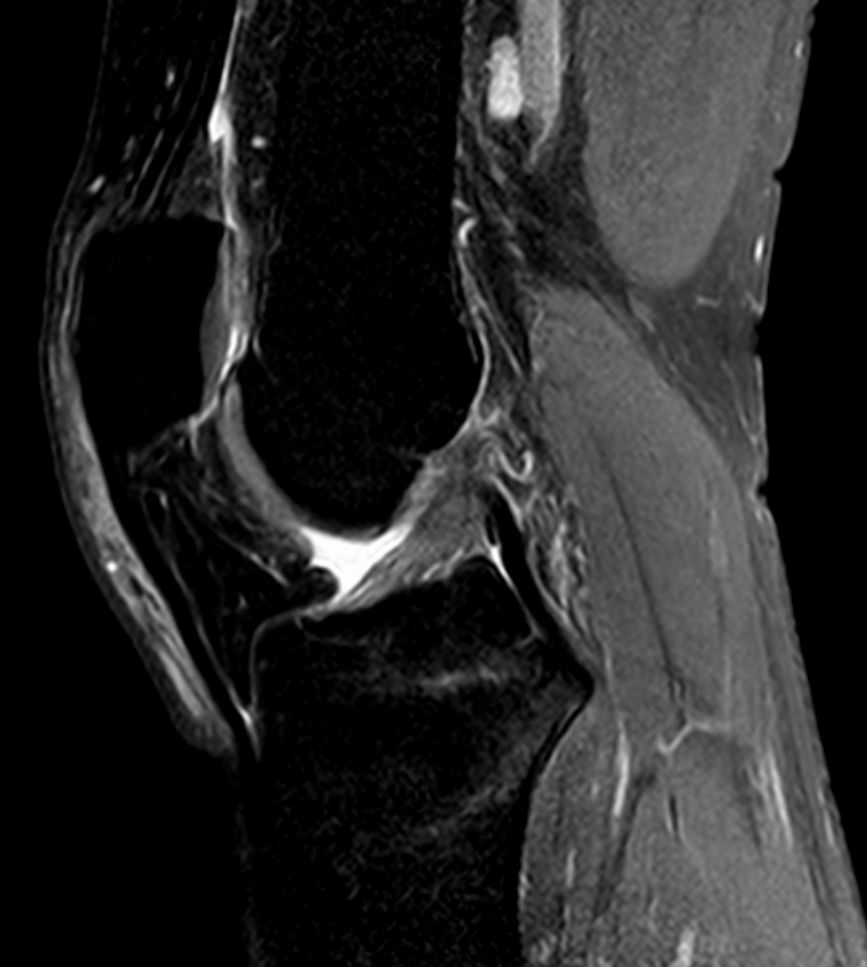
\includegraphics[height=44mm]{img/commons/acl_tear.jpg}
  \caption{ACL rupture, sagittal. A normal ACL is a dark, straight band; a ruptured one is interrupted or missing. Bright fluid fills the joint.}
\end{subfigure}\hfill
\begin{subfigure}[t]{0.33\linewidth}\centering
  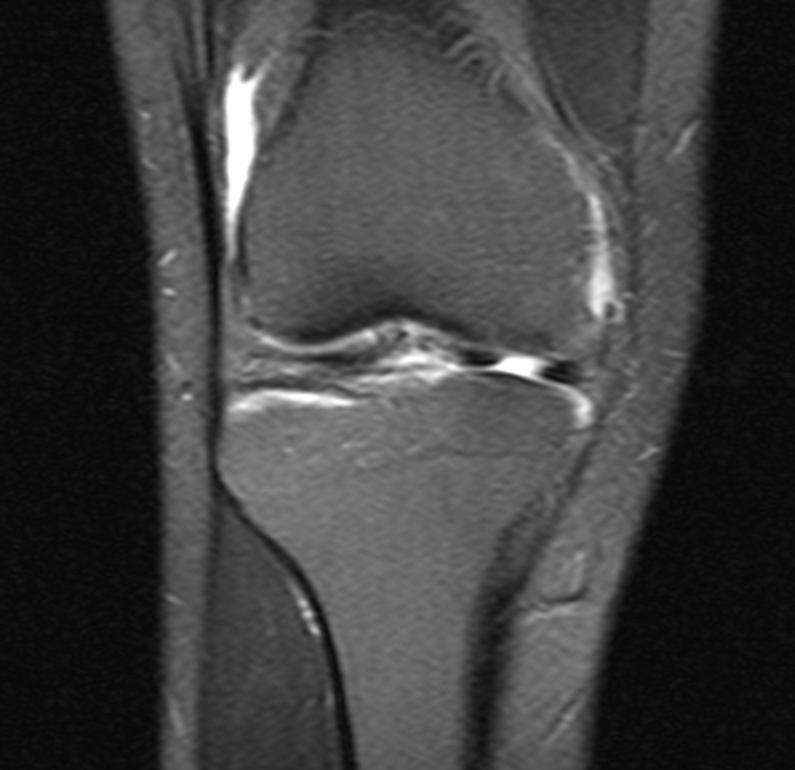
\includegraphics[height=44mm]{img/commons/meniscus_tear.jpg}
  \caption{Meniscus tear, coronal. A normal meniscus is a dark wedge; a tear shows up as a bright line inside it.}
\end{subfigure}\hfill
\begin{subfigure}[t]{0.31\linewidth}\centering
  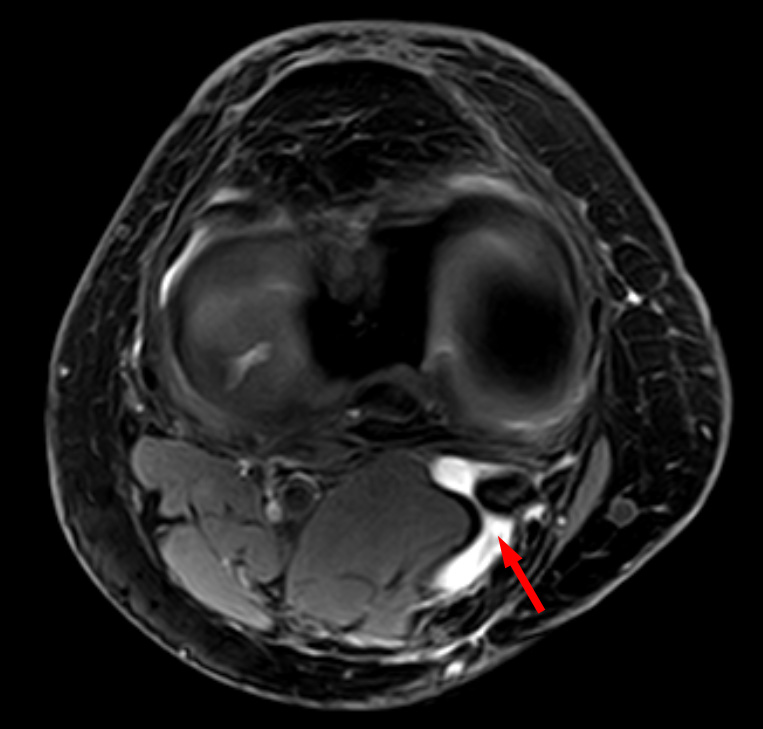
\includegraphics[height=44mm]{img/commons/baker_ax.jpg}
  \caption{Baker's cyst, axial (a slice across the leg). The arrow marks the channel between the cyst and the joint.}
\end{subfigure}
\caption{Three findings on real MRI images. All three images are fat-suppressed, so fluid is bright and fat is
dark (Chapter~\ref{ch:mri}). Images: Hellerhoff and Ciernik M, Wikimedia Commons, CC BY-SA (Appendix~\ref{app:credits}).}
\label{fig:realfindings}
\end{figure}

\begin{checkpoint}
\begin{itemize}
\done I can point to the femur, tibia, patella, both menisci, the ACL and the MCL on a drawing.
\done I know what medial, lateral and ``compartment'' mean.
\quiz Q2.1: A report says ``small joint effusion''. Is Effusion positive?
\quiz Q2.2: Which three findings share one rule about cartilage, and how do they differ?
\quiz Q2.3: Why might a model confuse Medial and Lateral Meniscus if it cannot tell a left knee from a right knee?
\end{itemize}
\end{checkpoint}

\chapter{MRI in fifteen minutes}
\label{ch:mri}

\begin{tldr}
\begin{itemize}
\item An MRI \textbf{series} is a stack of 2D slices; a knee \textbf{exam} has several series.
\item Each series is cut in one of three directions: \textbf{sagittal} (side view), \textbf{coronal} (front view),
      \textbf{axial} (cross-section).
\item The scanner settings (the \textbf{sequence}) decide what is bright. \textbf{Fluid-sensitive, fat-suppressed}
      series make fluid, swelling and tears bright: they are the ones that show most findings.
\item Pixels are small (\ca 0.4\,mm) but slices are thick (\ca 3.5\,mm), and brightness has \textbf{no units}.
\end{itemize}
\end{tldr}

\section{How MRI makes a picture, in three sentences}

The scanner is a strong magnet. Radio pulses make the hydrogen in the body's water and fat send back a weak
signal, and the scanner measures it point by point. How bright a tissue looks depends on how much water and fat
it holds \emph{and} on the timing of the radio pulses, so the same knee can be imaged in very different ways.

\section{Slices and stacks}

\begin{figure}[H]
\centering
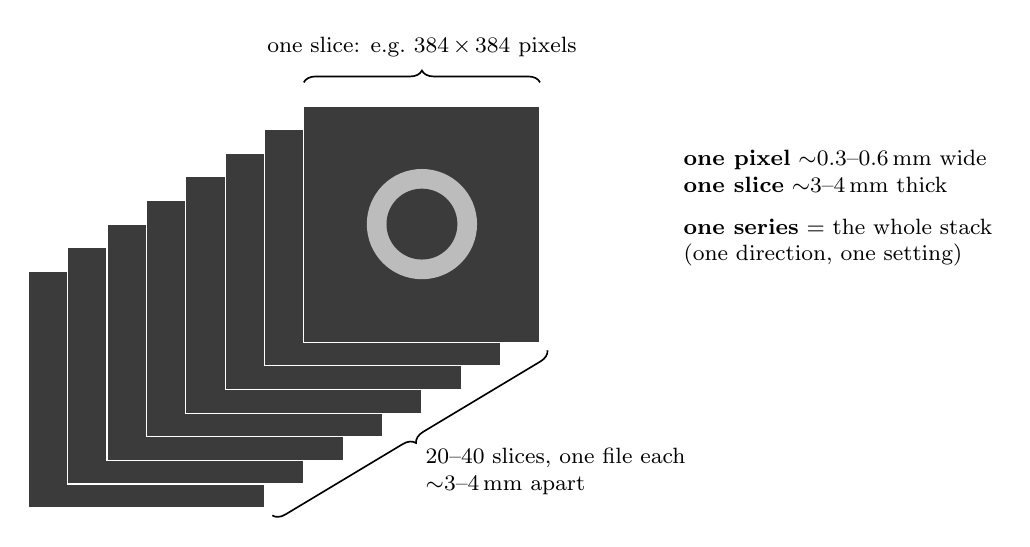
\begin{tikzpicture}[x=1mm,y=1mm]
  \foreach \k in {0,...,7} {
    \fill[dark!88, draw=white, line width=0.4pt] ({\k*5},{\k*3}) -- ++(30,0) -- ++(0,30) -- ++(-30,0) -- cycle;
    \fill[white!70!dark] ({\k*5+15},{\k*3+15}) circle (7);
    \fill[dark!88] ({\k*5+15},{\k*3+15}) circle (4.5);
  }
  \draw[decorate, decoration={brace, amplitude=1.5mm}, line width=0.6pt] (35,54) -- (65,54)
     node[midway, above=2mm, font=\footnotesize] {one slice: e.g.\ 384\,$\times$\,384 pixels};
  \draw[decorate, decoration={brace, amplitude=1.5mm, mirror}, line width=0.6pt] (31,-1) -- (66,20)
     node[midway, below right=1mm, font=\footnotesize, align=left] {20--40 slices, one file each\\ \ca 3--4\,mm apart};
  \node[anchor=west, font=\footnotesize, align=left] at (82,38) {\textbf{one pixel} \ca 0.3--0.6\,mm wide\\
     \textbf{one slice} \ca 3--4\,mm thick\\[2mm] \textbf{one series} = the whole stack\\ (one direction, one setting)};
\end{tikzpicture}
\caption{A series is a stack of slices. In the competition files every slice is a separate file.}
\end{figure}

\section{Three directions}

\begin{figure}[H]
\centering
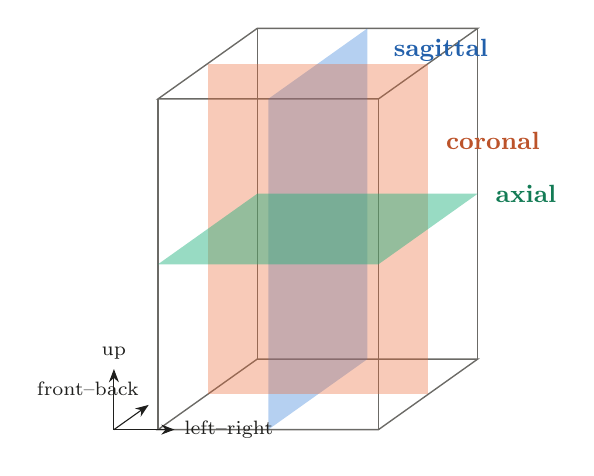
\begin{tikzpicture}[x={(1cm,0cm)}, y={(0.45cm,0.32cm)}, z={(0cm,1cm)}, scale=0.7]
  % a leg-shaped box, x = left-right, y = front-back, z = up-down
  \draw[muted, line width=0.5pt] (0,0,0) -- (4,0,0) -- (4,4,0) -- (0,4,0) -- cycle;
  \draw[muted, line width=0.5pt] (0,0,6) -- (4,0,6) -- (4,4,6) -- (0,4,6) -- cycle;
  \foreach \x/\y in {0/0,4/0,4/4,0/4} \draw[muted, line width=0.5pt] (\x,\y,0) -- (\x,\y,6);
  % planes
  \fill[us, opacity=0.35] (2,0,0) -- (2,4,0) -- (2,4,6) -- (2,0,6) -- cycle;
  \fill[them, opacity=0.35] (0,2,0) -- (4,2,0) -- (4,2,6) -- (0,2,6) -- cycle;
  \fill[third, opacity=0.45] (0,0,3) -- (4,0,3) -- (4,4,3) -- (0,4,3) -- cycle;
  \node[font=\small\bfseries, text=us!80!black, anchor=west] at (2.3,4,5.6) {sagittal};
  \node[font=\small\bfseries, text=them!80!black, anchor=west] at (4.15,2,4.6) {coronal};
  \node[font=\small\bfseries, text=third!70!black, anchor=west] at (4.15,4,3) {axial};
  \draw[-{Stealth}, ink] (-0.8,0,0) -- (0.3,0,0) node[right, font=\scriptsize] {left--right};
  \draw[-{Stealth}, ink] (-0.8,0,0) -- (-0.8,1.4,0) node[above left, font=\scriptsize] {front--back};
  \draw[-{Stealth}, ink] (-0.8,0,0) -- (-0.8,0,1.1) node[above, font=\scriptsize] {up};
\end{tikzpicture}\hspace{6mm}
\begin{minipage}[b]{0.52\linewidth}\small
\textcolor{us}{\textbf{Sagittal}}: slices from left to right. Each slice is a side view. Best for the ACL, the front and back of
the menisci, effusion.\par\medskip
\textcolor{them!85!black}{\textbf{Coronal}}: slices from front to back. Each slice is a front view. Best for the
MCL, the middle of the menisci, medial vs.\ lateral cartilage.\par\medskip
\textcolor{third!75!black}{\textbf{Axial}}: slices from bottom to top. Each slice is a cross-section of the
leg. Best for the kneecap (PF OA), Baker's cyst, synovitis.\par\bigskip
\end{minipage}
\caption{The three directions. Each one shows full detail within its slices and coarse detail across them,
so an exam needs all three.}
\label{fig:planes}
\end{figure}

\begin{figure}[H]
\centering
\begin{subfigure}[t]{0.33\linewidth}\centering
  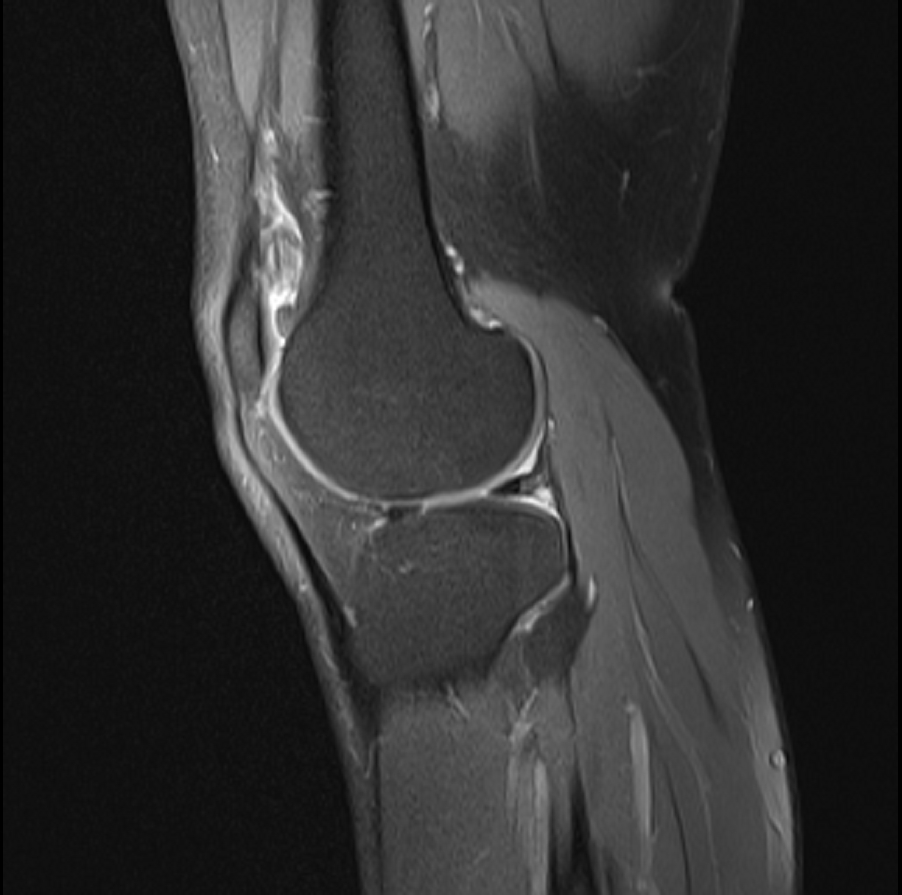
\includegraphics[height=46mm]{img/commons/sag_pd_fs.jpg}
  \caption{Sagittal (front of the knee on the left).}
\end{subfigure}\hfill
\begin{subfigure}[t]{0.25\linewidth}\centering
  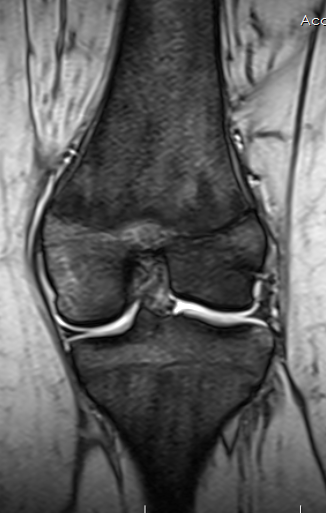
\includegraphics[height=46mm]{img/commons/cor_t2.png}
  \caption{Coronal.}
\end{subfigure}\hfill
\begin{subfigure}[t]{0.33\linewidth}\centering
  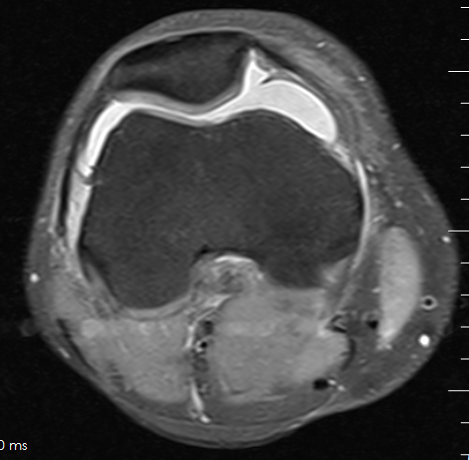
\includegraphics[height=46mm]{img/commons/ax_pd_fs.png}
  \caption{Axial (kneecap at the top).}
\end{subfigure}
\caption{One slice from each direction (three different people). Compare them with the drawings in
Figure~\ref{fig:anatomy}. Images: Ptrump16 and Nevit Dilmen, Wikimedia Commons, CC BY-SA.}
\label{fig:realplanes}
\end{figure}

\section{Sequences: what is bright and what is dark}

The radio-pulse timing is called the \term{sequence}. Knee exams use two families:

\begin{figure}[H]
\centering
\begin{subfigure}[t]{0.42\linewidth}\centering
  \begin{tikzpicture}
    \node[anchor=south west, inner sep=0] (a) at (0,0) {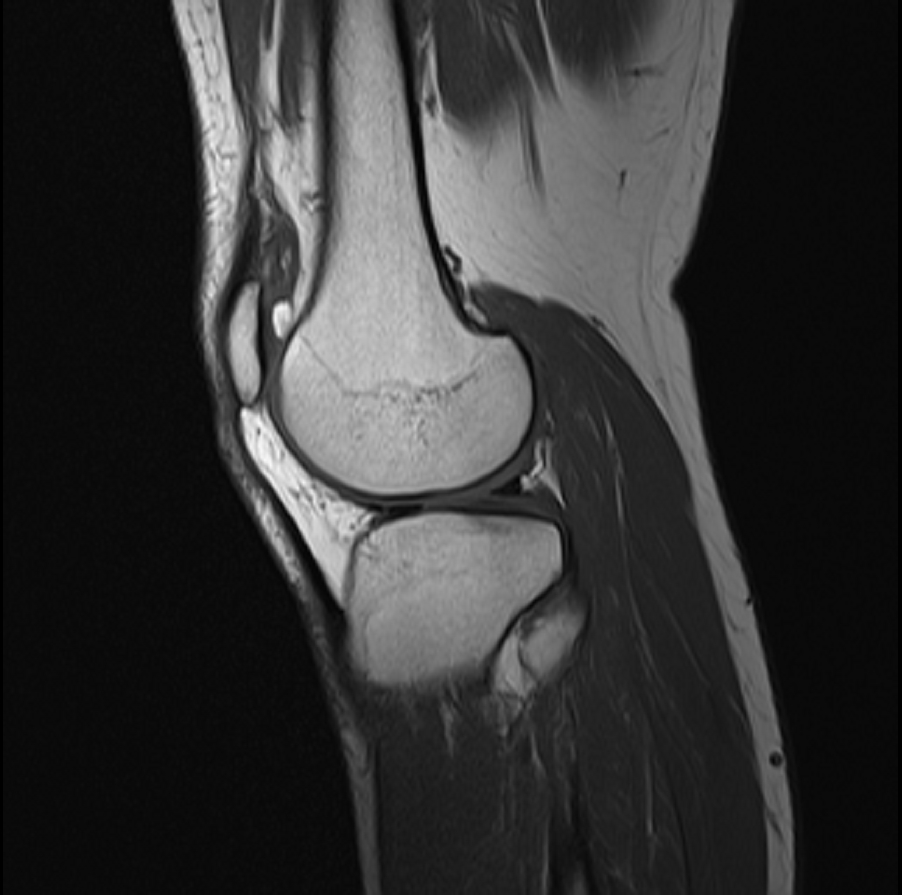
\includegraphics[height=56mm]{img/commons/sag_t1.jpg}};
    \begin{scope}[x={(a.south east)}, y={(a.north west)}]
      \draw[them, line width=1.1pt, -{Stealth}] (0.20,0.86) -- (0.41,0.66);
      \node[font=\scriptsize\bfseries, text=white, fill=them, inner sep=1.5pt, anchor=south] at (0.20,0.86) {bone marrow: bright};
    \end{scope}
  \end{tikzpicture}
  \caption{\textbf{T1}: fat is bright. The bone marrow (fatty) looks white; fluid is dark. Good for anatomy and
  fracture lines.}
\end{subfigure}\hspace{6mm}
\begin{subfigure}[t]{0.42\linewidth}\centering
  \begin{tikzpicture}
    \node[anchor=south west, inner sep=0] (b) at (0,0) {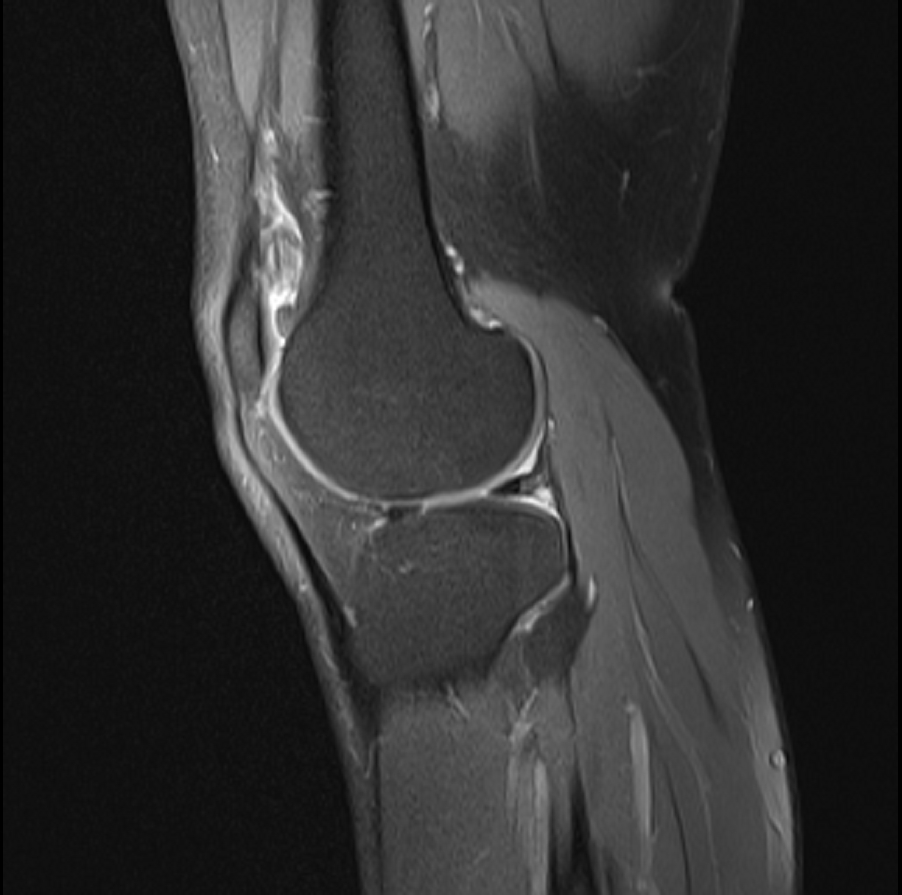
\includegraphics[height=56mm]{img/commons/sag_pd_fs.jpg}};
    \begin{scope}[x={(b.south east)}, y={(b.north west)}]
      \draw[us, line width=1.1pt, -{Stealth}] (0.12,0.86) -- (0.28,0.69);
      \node[font=\scriptsize\bfseries, text=white, fill=us, inner sep=1.5pt, anchor=south] at (0.12,0.86) {fluid: bright};
      \draw[them, line width=1.1pt, -{Stealth}] (0.72,0.86) -- (0.47,0.60);
      \node[font=\scriptsize\bfseries, text=white, fill=them, inner sep=1.5pt, anchor=south] at (0.72,0.86) {marrow: grey};
    \end{scope}
  \end{tikzpicture}
  \caption{\textbf{PD fat-suppressed}: fat is switched off. Marrow turns grey; fluid and swelling stand out white.
  Good for tears, effusion, bone bruises.}
\end{subfigure}
\caption{The same knee, the same slice position, two sequences. Images: Ptrump16, Wikimedia Commons, CC BY-SA 4.0.}
\label{fig:t1pd}
\end{figure}

\begin{center}\small
\begin{tabular}{lcc}
\toprule
Tissue & T1 & fluid-sensitive, fat-suppressed \\
\midrule
fat (under the skin, bone marrow) & \textbf{bright} & dark \\
fluid (effusion, cysts) & dark & \textbf{bright} \\
swelling / edema (bone bruise) & greyish & \textbf{bright} \\
ligaments, tendons, menisci & dark & dark (a tear = a bright line) \\
cartilage, muscle & grey & grey \\
\bottomrule
\end{tabular}
\end{center}

\begin{keyidea}
Most of the 12 findings are ``water where it should not be'': fluid in the joint, swelling in the bone, fluid
seeping into a torn ligament or meniscus. A \textbf{fluid-sensitive, fat-suppressed} series makes exactly that
bright. That is why our pipeline used those series first.
\end{keyidea}

\begin{wordcheck}
\term{PD} (proton density), \term{T1}, \term{T2}: names of sequences. \term{Fat suppression} (``fat-sat'',
``FS''): a trick that removes the fat signal. \term{Fluid-sensitive}: a sequence where water is bright (PD or T2,
usually with fat suppression). The competition's \code{train\_series.csv} tells you, for every series, its plane,
whether it is fluid-sensitive and whether fat is suppressed.
\end{wordcheck}

\section{A typical knee exam}

\begin{center}\small
\begin{tabular}{llll}
\toprule
Series & Plane & Sequence & Used by us? \\
\midrule
\textbf{sag fluid} & sagittal & PD fat-suppressed & \cmark\ role \code{sag\_fs} \\
\textbf{cor fluid} & coronal & PD or T2 fat-suppressed & \cmark\ role \code{cor\_fs} \\
\textbf{ax fluid} & axial & PD fat-suppressed & \cmark\ role \code{ax\_fs} \\
sag structural & sagittal & T1 or PD without fat suppression & \xmark\ (the winners did) \\
cor structural & coronal & T1 & \xmark\ (the winners did) \\
\bottomrule
\end{tabular}
\end{center}
The training set has 24,371 series for 4,407 exams: about \textbf{5.5 series per exam}. Sites differ: some scan
more, some fewer, and they name and store them differently.

\section{Voxels are not cubes}

\begin{figure}[H]
\centering
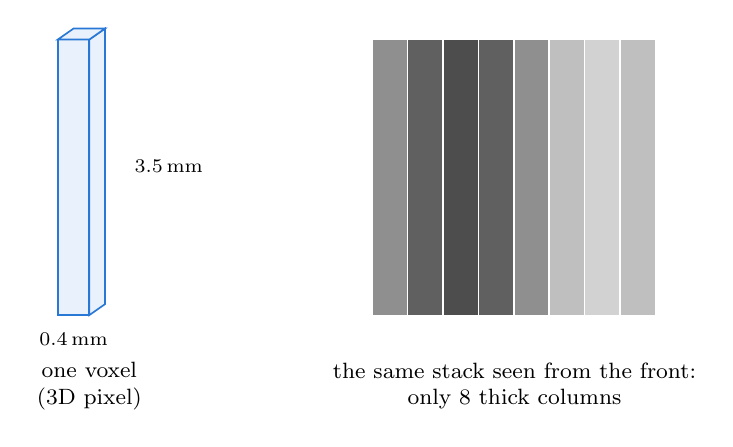
\begin{tikzpicture}[x={(1cm,0cm)}, y={(0.5cm,0.35cm)}, z={(0cm,1cm)}]
  % a thin, tall voxel
  \foreach \f in {{(0,0,0)--(0.4,0,0)--(0.4,0,3.5)--(0,0,3.5)--cycle},
                  {(0.4,0,0)--(0.4,0.4,0)--(0.4,0.4,3.5)--(0.4,0,3.5)--cycle},
                  {(0,0,3.5)--(0.4,0,3.5)--(0.4,0.4,3.5)--(0,0.4,3.5)--cycle}}
    \filldraw[fill=keyfill, draw=accent, line width=0.6pt] \f;
  \node[font=\scriptsize, anchor=north] at (0.2,0,-0.1) {0.4\,mm};
  \node[font=\scriptsize, anchor=west] at (0.65,0.4,1.75) {3.5\,mm};
  \node[font=\footnotesize, align=center] at (0.4,0,-0.9) {one voxel\\ (3D pixel)};
  % a reformat: sagittal stack viewed from the front is blocky
  \begin{scope}[xshift=4cm]
    \foreach \i in {0,...,7} {
      \pgfmathsetmacro{\g}{50+30*sin(\i*45)}
      \fill[dark!\g] ({\i*0.45},0,0) rectangle ({\i*0.45+0.43},0,3.5);
    }
    \node[font=\footnotesize, align=center] at (1.8,0,-0.9) {the same stack seen from the front:\\ only 8 thick columns};
  \end{scope}
\end{tikzpicture}
\caption{Within a slice the detail is fine; across slices it is about ten times coarser. Turning a sagittal stack
into a front view gives a blocky picture.}
\end{figure}

\begin{why}
This is why most solutions (ours and the winners') use \textbf{2D image models on single slices or on a few
neighbouring slices} (``2.5D'', Chapter~\ref{ch:toolbox}) instead of true 3D models, and why the exam includes
three directions: each direction is sharp where the others are coarse.
\end{why}

\section{MRI has no units}

In a CT scan, water is always 0 on the brightness scale. In MRI the raw numbers depend on the scanner, the coil,
the sequence and the patient. Only \emph{relative} brightness inside one series means anything.

\begin{figure}[H]
\centering
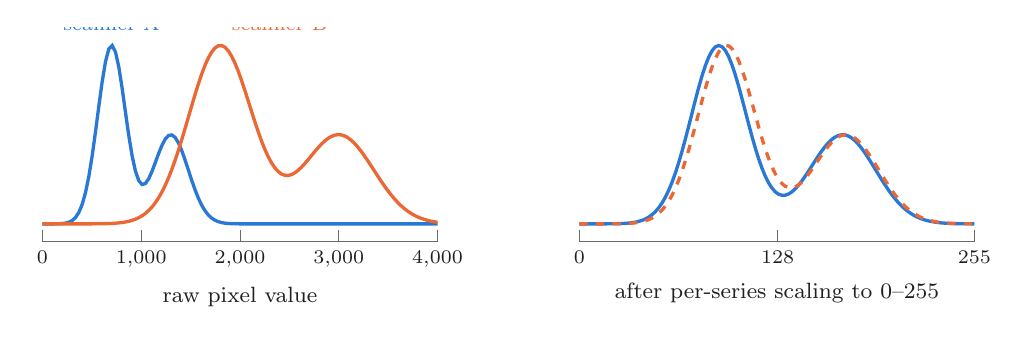
\begin{tikzpicture}
\begin{groupplot}[group style={group size=2 by 1, horizontal sep=18mm}, width=6.6cm, height=4.3cm,
    ytick=\empty, axis x line*=bottom, axis y line=none, xlabel style={font=\footnotesize}]
  \nextgroupplot[xlabel={raw pixel value}, xmin=0, xmax=4000, xtick={0,1000,2000,3000,4000},
                 scaled x ticks=false, xticklabel style={font=\scriptsize}]
    \addplot[us, line width=1.2pt, domain=0:4000, samples=120] {exp(-((x-700)/200)^2) + 0.5*exp(-((x-1300)/250)^2)};
    \addplot[them, line width=1.2pt, domain=0:4000, samples=120] {exp(-((x-1800)/450)^2) + 0.5*exp(-((x-3000)/500)^2)};
    \node[font=\scriptsize, text=us] at (axis cs:700,1.12) {scanner A};
    \node[font=\scriptsize, text=them] at (axis cs:2400,1.12) {scanner B};
  \nextgroupplot[xlabel={after per-series scaling to 0--255}, xmin=0, xmax=255, xtick={0,128,255},
                 xticklabel style={font=\scriptsize}]
    \addplot[us, line width=1.2pt, domain=0:255, samples=120] {exp(-((x-90)/25)^2) + 0.5*exp(-((x-170)/30)^2)};
    \addplot[them, line width=1.2pt, dashed, domain=0:255, samples=120] {exp(-((x-95)/26)^2) + 0.5*exp(-((x-172)/30)^2)};
\end{groupplot}
\end{tikzpicture}
\caption{The same two tissues on two scanners (schematic). Raw values are not comparable (left). Scaling every
series by its own percentiles lines them up (right). Chapter~\ref{ch:cache} shows how we did it.}
\end{figure}

\begin{checkpoint}
\begin{itemize}
\done I can name the three directions and say what each one is good for.
\done I know why fluid-sensitive, fat-suppressed series matter for this task.
\quiz Q3.1: On a T1 image, is a bone bruise easy to see? On a fat-suppressed PD image?
\quiz Q3.2: Why can't you use one fixed brightness rule (``above 1,000 = fluid'') for all exams?
\quiz Q3.3: A model sees only sagittal images. Which finding might it struggle with most, and why?
\end{itemize}
\end{checkpoint}

\chapter{The data}
\label{ch:data}
\whereami{1}

\begin{tldr}
\begin{itemize}
\item 4,407 training exams, 24,371 series, one \textbf{DICOM} file per slice. About 1,300 hidden test exams.
\item Only \textbf{58} training exams have the 12 labels from doctors (``gold''). The other \textbf{4,349} have a
      free-text \textbf{radiology report} in one of 12 languages, and no labels.
\item The test exams have \textbf{images only}: no report.
\item So the real first task is: \textbf{turn 4,349 reports into labels}, then train an image model on them.
\end{itemize}
\end{tldr}

\section{Folders: study, series, slice}

\begin{figure}[H]
\centering
\begin{tikzpicture}[x=1mm,y=1mm, every node/.style={font=\footnotesize}]
  \node[anchor=west] at (0,0) {\faFolder\ \code{train\_series/}};
  \draw[muted] (2,-2) -- (2,-26);
  \draw[muted] (2,-6) -- (6,-6); \node[anchor=west] at (6,-6) {\faFolder\ \code{<StudyInstanceUID>/}};
  \node[anchor=west, text=us] at (62,-6) {\faArrowLeft\ one \textbf{study} = one exam = one row of labels};
  \draw[muted] (9,-8) -- (9,-24);
  \draw[muted] (9,-12) -- (13,-12); \node[anchor=west] at (13,-12) {\faFolder\ \code{<SeriesInstanceUID>/}};
  \node[anchor=west, text=us] at (62,-12) {\faArrowLeft\ one \textbf{series} = one 3D stack (e.g.\ sagittal PD fat-sat)};
  \draw[muted] (16,-14) -- (16,-21);
  \draw[muted] (16,-17) -- (20,-17); \node[anchor=west] at (20,-17) {\faFile\ \code{<SOPInstanceUID>.dcm}};
  \node[anchor=west, text=us] at (62,-17) {\faArrowLeft\ one \textbf{slice} (one 2D image + header)};
  \draw[muted] (16,-21) -- (20,-21); \node[anchor=west, text=muted] at (20,-21) {\ldots\ 20--40 more slices};
  \draw[muted] (9,-24) -- (13,-24); \node[anchor=west, text=muted] at (13,-24) {\ldots\ \ca 5 more series};
  \draw[muted] (2,-26) -- (6,-26); \node[anchor=west, text=muted] at (6,-26) {\ldots\ 4,406 more studies};
\end{tikzpicture}
\caption{The folder tree. The long numbers (UIDs) are random identifiers; they tell you nothing by themselves.
The CSV files link them to labels and to series descriptions.}
\end{figure}

\section{One DICOM file}

\term{DICOM} is the file format of medical imaging. A \code{.dcm} file has two parts:

\begin{figure}[H]
\centering
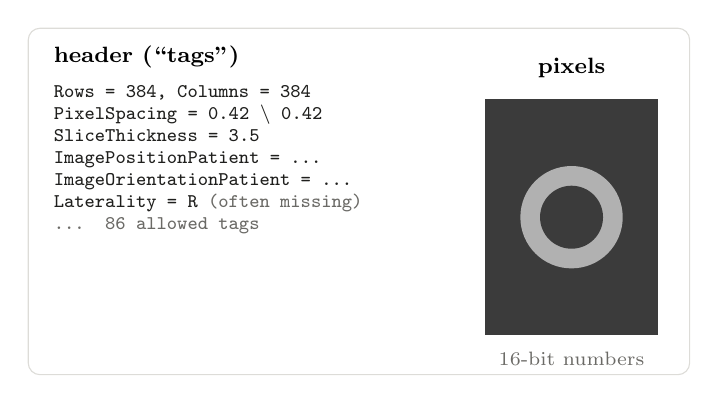
\begin{tikzpicture}[x=1mm,y=1mm]
  \node[draw=grid, fill=white, rounded corners=1.5mm, minimum width=84mm, minimum height=44mm] (f) at (0,0) {};
  \node[anchor=north west, font=\footnotesize\bfseries] at (-40,21) {header (``tags'')};
  \node[anchor=north west, font=\scriptsize\ttfamily, align=left, text=ink] at (-40,16)
    {Rows = 384, Columns = 384\\ PixelSpacing = 0.42 \textbackslash{} 0.42\\ SliceThickness = 3.5\\
     ImagePositionPatient = ...\\ ImageOrientationPatient = ...\\ Laterality = R \textcolor{muted}{(often missing)}\\
     \textcolor{muted}{... 86 allowed tags}};
  \fill[dark!88] (16,-17) rectangle (38,13);
  \fill[white!65!dark] (27,-2) circle (6.5);
  \fill[dark!88] (27,-2) circle (4);
  \node[font=\footnotesize\bfseries] at (27,17) {pixels};
  \node[font=\scriptsize, text=muted] at (27,-20) {16-bit numbers};
\end{tikzpicture}
\caption{A DICOM file = a dictionary of metadata + the image. The header matters as much as the pixels: it
says where the slice sits in the body, in millimetres.}
\end{figure}

\begin{center}\small
\begin{tabularx}{\linewidth}{l>{\raggedright\arraybackslash}X}
\toprule
Tag & Why we need it \\
\midrule
\code{ImagePositionPatient} & 3D position of the slice's corner (mm). Sort slices by this, never by file name. \\
\code{ImageOrientationPatient} & directions of the image rows and columns in the body. Tells the plane, and whether the image is flipped or rotated. \\
\code{PixelSpacing}, \code{SliceThickness} & size of a pixel and of a slice in mm. Needed to resize every series to the same physical scale. \\
\code{Laterality} & left or right knee. Missing in about half of the exams. \\
\bottomrule
\end{tabularx}
\end{center}

\begin{watchout}
The competition's files keep only 86 ``allowed'' header tags, and sites fill them inconsistently. Every tag can
be missing; read them defensively.
\end{watchout}

\section{The tables}

\begin{figure}[H]
\centering
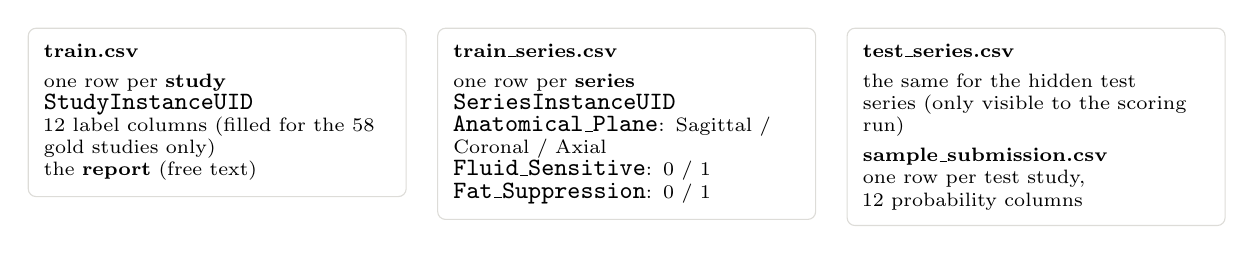
\begin{tikzpicture}[x=1mm,y=1mm,
  tbl/.style={draw=grid, fill=white, rounded corners=1mm, align=left, font=\scriptsize, inner sep=2mm, anchor=north west}]
  \node[tbl, text width=44mm] at (0,0) {\textbf{train.csv}\\[1mm] one row per \textbf{study}\\
     \code{StudyInstanceUID}\\ 12 label columns (filled for the 58 gold studies only)\\ the \textbf{report} (free text)};
  \node[tbl, text width=44mm] at (52,0) {\textbf{train\_series.csv}\\[1mm] one row per \textbf{series}\\
     \code{SeriesInstanceUID}\\ \code{Anatomical\_Plane}: Sagittal / Coronal / Axial\\ \code{Fluid\_Sensitive}: 0 / 1\\
     \code{Fat\_Suppression}: 0 / 1};
  \node[tbl, text width=44mm] at (104,0) {\textbf{test\_series.csv}\\[1mm] the same for the hidden test\\
     series (only visible to the scoring run)\\[1mm] \textbf{sample\_submission.csv}\\ one row per test study,\\ 12 probability columns};
\end{tikzpicture}
\caption{The CSV files. \code{train\_series.csv} is precious: it already says which series is which, so we did
not have to guess from the images.}
\end{figure}

\section{The numbers}

\begin{figure}[H]
\centering
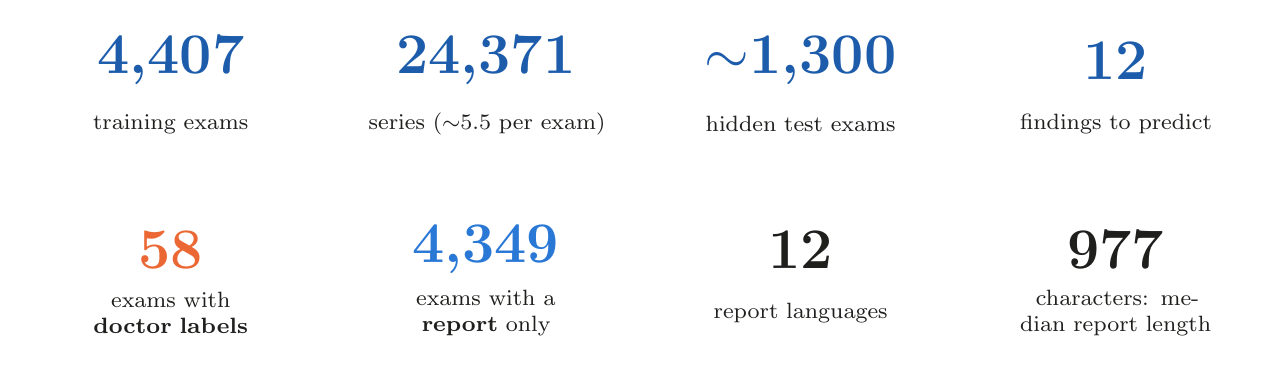
\begin{tikzpicture}[x=1mm,y=1mm,
  big/.style={font=\fontsize{20}{22}\selectfont\bfseries, text=accentdark},
  small/.style={font=\footnotesize, text=ink, align=center, text width=34mm}]
  \foreach \x/\n/\t in {0/{4,407}/{training exams}, 40/{24,371}/{series (\ca 5.5 per exam)}, 80/{\ca 1,300}/{hidden test exams},
                        120/12/{findings to predict}} {
    \node[big] at (\x,8) {\n};
    \node[small] at (\x,0) {\t};
  }
  \foreach \x/\n/\t/\c in {0/58/{exams with \textbf{doctor labels}}/them, 40/{4,349}/{exams with a \textbf{report} only}/us,
                           80/12/{report languages}/ink, 120/977/{characters: median report length}/ink} {
    \node[big, text=\c] at (\x,-16) {\n};
    \node[small] at (\x,-24) {\t};
  }
\end{tikzpicture}
\end{figure}

\section{Who labelled what}

\begin{figure}[H]
\centering
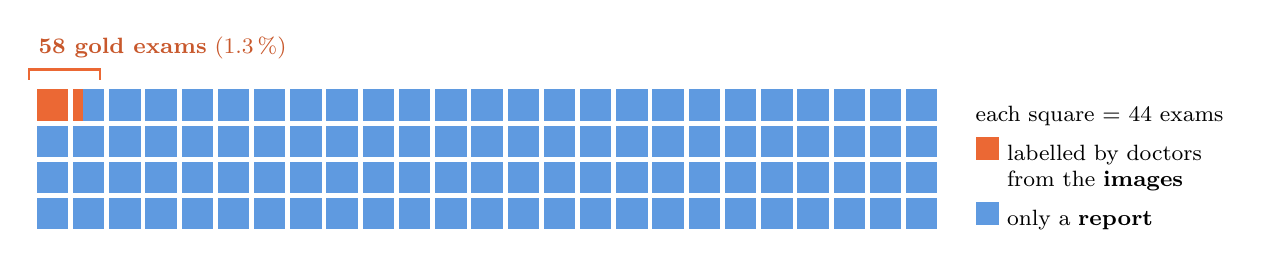
\begin{tikzpicture}[x=1mm,y=1mm]
  \foreach \i in {0,...,99} {
    \pgfmathsetmacro{\c}{mod(\i,25)}
    \pgfmathsetmacro{\r}{int(\i/25)}
    \fill[us!75] ({\c*4.6},{-\r*4.6}) rectangle ++(4,4);
  }
  % 58 of 4,407 = 1.3 squares of 44 studies each
  \fill[them] (0,0) rectangle ++(4,4);
  \fill[them] (4.6,0) rectangle ++(1.3,4);
  \draw[them, line width=0.8pt] (-1,5.2) -- (-1,6.5) -- (8,6.5) -- (8,5.2);
  \node[anchor=south west, font=\footnotesize, text=them!85!black] at (-1,6.6) {\textbf{58 gold exams} (1.3\,\%)};
  \node[anchor=west, font=\footnotesize, align=left] at (118,-6) {each square = 44 exams\\[1mm]
     \textcolor{them}{\rule{3mm}{3mm}} labelled by doctors\\ \hspace*{4mm}from the \textbf{images}\\[1mm]
     \textcolor{us!75}{\rule{3mm}{3mm}} only a \textbf{report}};
\end{tikzpicture}
\caption{The training set. Almost everything has to be learned from reports.}
\label{fig:waffle}
\end{figure}

\paragraph{The 58 gold exams.} Two musculoskeletal radiologists read the \emph{images} independently, a third
settled disagreements, and they applied the strict thresholds of Figure~\ref{fig:thresholds}. These are the only
labels we can fully trust.

\paragraph{The 4,349 report-only exams.} The report is what the hospital's radiologist wrote at the time,
in their own language and style. It mentions what that radiologist thought worth mentioning, with their own
severity words.

\begin{figure}[H]
\centering
\begin{tikzpicture}
\begin{axis}[xbar, width=11cm, height=6.2cm, bar width=2.6mm, xmin=0, xmax=1950,
    symbolic y coords={Thai,Serbian,Bulgarian,French,Dutch,Russian,German,Greek,Croatian,Turkish,Spanish,English},
    ytick=data, y tick label style={font=\footnotesize}, xtick=\empty, axis x line=none, axis y line*=left,
    nodes near coords, nodes near coords style={font=\scriptsize, anchor=west}, enlarge y limits=0.06]
  \addplot[barus] table[x=n, y=lang] {figdata/languages.dat};
\end{axis}
\end{tikzpicture}
\caption{Report languages of the 4,349 report-only exams. Any labelling method has to read all of them.}
\label{fig:languages}
\end{figure}

\begin{example}
A made-up report for our imaginary \textbf{Study K} (real reports are longer, about 1,000 characters):
\begin{quote}\small\itshape
Complete rupture of the anterior cruciate ligament. Bone contusion of the lateral femoral condyle and the
posterolateral tibial plateau. Moderate joint effusion. Menisci intact. Collateral ligaments intact.
Cartilage preserved.
\end{quote}
A careful reader would turn this into: ACL \textbf{yes}, Contusion \textbf{yes}, Effusion \textbf{yes}
(moderate), both menisci \textbf{no}, MCL \textbf{no}, all three OA \textbf{no}, and \ldots\ Synovitis, Baker's,
Fracture: \textbf{not mentioned}. What do you do with ``not mentioned''? Chapter~\ref{ch:labels} answers that.
\end{example}

\section{How common is each finding?}

\begin{figure}[H]
\centering
\begin{tikzpicture}
\begin{axis}[ybar, width=\linewidth, height=6cm, bar width=3.2mm, ymin=0, ymax=70,
    symbolic x coords={ACL,MCL,Med.~meniscus,Lat.~meniscus,Med.~OA,Lat.~OA,PF OA,Effusion,Synovitis,Baker's,Contusion,Fracture},
    xtick=data, x tick label style={font=\scriptsize, rotate=35, anchor=north east}, ylabel={\% of exams positive},
    ylabel style={font=\footnotesize}, ymajorgrids, legend style={at={(0.02,0.98)}, anchor=north west},
    enlarge x limits=0.05]
  \addplot[barthem] table[x=finding, y=gold] {figdata/prevalence.dat};
  \addplot[barus] table[x=finding, y=pool] {figdata/prevalence.dat};
  \legend{{58 gold exams (doctors)}, {4,349 report exams (our labels $>$ 0.5)}}
\end{axis}
\end{tikzpicture}
\caption{Each finding is about three times more common in the gold set than in the report set. The organisers
chose the gold exams to contain enough positives. Synovitis stands out: 47\,\% in gold, 10\,\% in our labels,
because reports rarely mention it.}
\label{fig:prevalence}
\end{figure}

\begin{watchout}
Because the gold set is enriched, a model's \emph{average} probabilities on gold look ``too low'' even when the
model is fine. AUC does not care (it only looks at order), but anything that relies on calibrated probabilities
would.
\end{watchout}

\section{The test set has no reports}

\begin{figure}[H]
\centering
\begin{tikzpicture}[x=1mm,y=1mm,
  box/.style={draw=grid, rounded corners=1.5mm, minimum height=13mm, align=center, font=\footnotesize, fill=white}]
  \node[font=\small\bfseries] at (-6,9) {training};
  \node[box, minimum width=34mm] at (30,9) {\faImage\ images};
  \node[box, minimum width=34mm, draw=us, line width=0.8pt] at (70,9) {\faFile\ report};
  \node[box, minimum width=34mm] at (110,9) {\faTag\ labels (58 only)};
  \node[font=\small\bfseries] at (-6,-9) {test};
  \node[box, minimum width=34mm] at (30,-9) {\faImage\ images};
  \node[box, minimum width=34mm, dashed, text=muted] at (70,-9) {no report};
  \node[box, minimum width=34mm, dashed, text=muted] at (110,-9) {no labels};
\end{tikzpicture}
\caption{At test time only the images exist. The report can teach the model during training, but the model has
to work from images alone.}
\end{figure}

\begin{keyidea}
Every solution in this competition has the same two steps:
\textbf{(1)} turn the reports (and maybe the images) of the 4,349 exams into labels;
\textbf{(2)} train an image model on those labels.
The image model can never be much better than its labels. Chapter~\ref{ch:labels} is step 1, Chapters
\ref{ch:cache}--\ref{ch:model} are step 2.
\end{keyidea}

\begin{wordcheck}
\term{Weak supervision}: training on labels that are cheaper but noisier than the real thing (here: labels read
from reports instead of doctors' image labels). \term{Gold labels}: the trusted reference labels (here: the 58).
\end{wordcheck}

\begin{checkpoint}
\begin{itemize}
\done I can describe the path from a folder of \code{.dcm} files to one study with its series.
\done I know which exams have labels, which have reports, and what the test set has.
\quiz Q4.1: Why sort slices by \code{ImagePositionPatient} rather than by file name?
\quiz Q4.2: Our labels say 11\,\% of exams have an ACL tear, the gold set says 41\,\%. Does that mean our labels
      are wrong?
\quiz Q4.3: Why can't the model simply read the report at test time?
\end{itemize}
\end{checkpoint}


\part{Machine-learning fundamentals}
\chapter{The machine-learning toolbox}
\label{ch:toolbox}

\begin{tldr}
\begin{itemize}
\item A model is a function with millions of adjustable numbers (\textbf{weights}). Training nudges them until the
      outputs match the labels.
\item Image models are \textbf{CNNs}: a pretrained \textbf{backbone} turns an image into a feature vector, a small
      \textbf{head} turns features into the 12 outputs.
\item Knee MRI is fed slice by slice (\textbf{2D}) or three neighbouring slices at a time (\textbf{2.5D}); the
      slice results are \textbf{pooled} into one answer per study.
\item Honest testing needs data the model never trained on: \textbf{cross-validation}. Averaging several models
      (\textbf{ensembling}) almost always helps a little.
\end{itemize}
\end{tldr}

\section{A model is a function with knobs}

\begin{figure}[H]
\centering
\begin{tikzpicture}[x=0.86mm,y=1mm]
  \node[draw=grid, fill=white, rounded corners=1.5mm, minimum width=24mm, minimum height=16mm, align=center,
        font=\footnotesize] (x) at (0,0) {\faImage\\ images\\ of one study};
  \node[draw=accent, fill=keyfill, rounded corners=2mm, minimum width=44mm, minimum height=22mm] (f) at (45,0) {};
  \node[font=\small\bfseries] at (45,6) {$f_{\theta}$};
  \foreach \i in {0,...,6} {
    \draw[accent, line width=0.6pt] ({29+\i*5.3},-5) circle (1.6);
    \draw[accent, line width=0.8pt] ({29+\i*5.3},-5) -- ++({90-\i*37}:1.6);
  }
  \node[font=\scriptsize, text=muted] at (45,-10) {millions of knobs $\theta$ (weights)};
  \node[draw=grid, fill=white, rounded corners=1.5mm, minimum width=24mm, minimum height=16mm, align=center,
        font=\footnotesize] (y) at (90,0) {12 numbers\\ (one per finding)};
  \draw[-{Stealth[length=2mm]}, line width=0.8pt, muted] (x) -- (f);
  \draw[-{Stealth[length=2mm]}, line width=0.8pt, muted] (f) -- (y);
  \node[draw=them, fill=whyfill, rounded corners=1.5mm, font=\footnotesize, align=center] (l) at (90,-22) {labels\\ (what we want)};
  \draw[{Stealth[length=2mm]}-{Stealth[length=2mm]}, them, line width=0.8pt, dashed] (y) -- (l)
     node[midway, right, font=\scriptsize] {compare};
  \draw[-{Stealth[length=2mm]}, them, line width=0.8pt] (l.west) -- (60,-22) -- (52,-13)
     node[pos=0.3, below, font=\scriptsize, text=them!85!black] {turn the knobs a little};
\end{tikzpicture}
\caption{Training in one picture: compare the outputs with the labels, then turn every knob a little in the
direction that reduces the difference. Repeat many thousands of times.}
\end{figure}

\begin{wordcheck}
\term{Weights} (parameters): the adjustable numbers inside the model. EfficientNet-B0, our main model, has about
5 million; the winners' models have 30--120 million. \term{Training}: adjusting them. \term{Inference}: using the
trained model on new data.
\end{wordcheck}

\section{How a CNN sees: filters}

A \term{convolutional neural network} (CNN) looks at an image through many small \term{filters}. A filter is a
3\,$\times$\,3 grid of weights that slides over the image; at each position it multiplies and adds, producing one
number. The result is a new image, a \term{feature map}, which is bright where the filter's pattern occurs.

\begin{figure}[H]
\centering
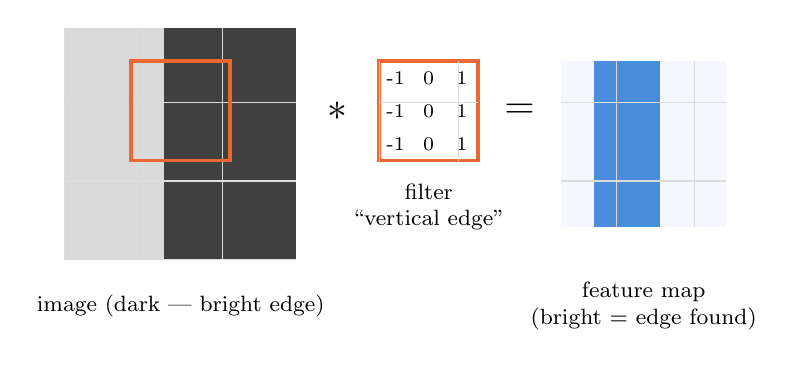
\begin{tikzpicture}[x=4.2mm,y=4.2mm]
  % input image 7x7
  \foreach \i in {0,...,6} \foreach \j in {0,...,6} {
    \pgfmathsetmacro{\v}{(\i<3) ? 15 : 75}
    \fill[black!\v] (\i,\j) rectangle ++(1,1);
  }
  \draw[grid] (0,0) grid (7,7);
  \draw[them, line width=1.4pt] (2,3) rectangle (5,6);
  \node[font=\footnotesize, align=center] at (3.5,-1.4) {image (dark | bright edge)};
  % filter
  \begin{scope}[xshift=10.5cm/4.2]
  \end{scope}
  \foreach \i/\w in {0/-1,1/0,2/1} \foreach \j in {0,1,2} {
    \fill[white] (\i+9.5,\j+3) rectangle ++(1,1);
    \node[font=\scriptsize] at (\i+10,\j+3.5) {\w};
  }
  \draw[them, line width=1.4pt] (9.5,3) rectangle (12.5,6);
  \draw[grid] (9.5,3) grid (12.5,6);
  \node[font=\footnotesize, align=center] at (11,1.6) {filter\\ ``vertical edge''};
  \node[font=\Large] at (8.25,4.5) {$\ast$};
  \node[font=\Large] at (13.75,4.5) {$=$};
  % feature map 5x5
  \foreach \i in {0,...,4} \foreach \j in {0,...,4} {
    \pgfmathsetmacro{\v}{(\i==1 || \i==2) ? 85 : 5}
    \fill[us!\v] (\i+15,\j+1) rectangle ++(1,1);
  }
  \draw[grid] (15,1) grid (20,6);
  \node[font=\footnotesize, align=center] at (17.5,-1.4) {feature map\\ (bright = edge found)};
\end{tikzpicture}
\caption{One filter finds vertical edges. A CNN learns hundreds of filters per layer and stacks dozens of layers:
early layers find edges, middle layers textures, deep layers whole structures (``a meniscus'', ``fluid'').}
\end{figure}

\section{Backbone and head}

\begin{figure}[H]
\centering
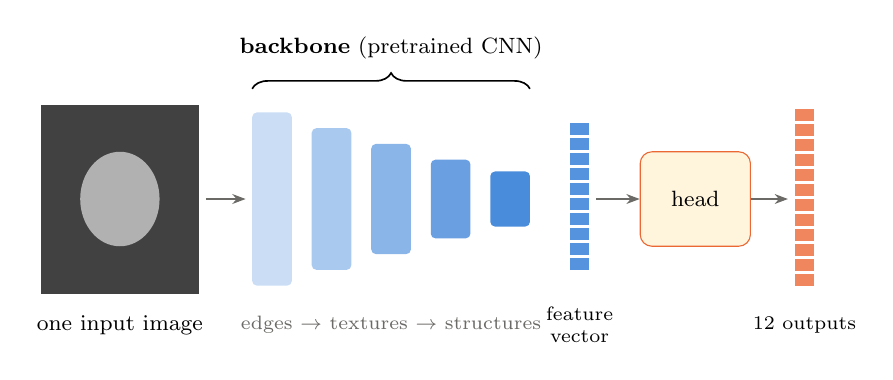
\begin{tikzpicture}[x=0.84mm,y=1mm]
  \fill[dark!85] (0,-12) rectangle (24,12);
  \fill[white!65!dark] (12,0) circle (6);
  \node[font=\footnotesize] at (12,-16) {one input image};
  % backbone: shrinking blocks
  \foreach \i/\h in {0/22,1/18,2/14,3/10,4/7} {
    \fill[us!\the\numexpr 25+\i*15\relax, rounded corners=0.6mm] ({32+\i*9},{-\h/2}) rectangle ++(6,\h);
  }
  \draw[decorate, decoration={brace, amplitude=2mm}, line width=0.6pt] (32,14) -- (74,14)
     node[midway, above=2.5mm, font=\footnotesize] {\textbf{backbone} (pretrained CNN)};
  \node[font=\scriptsize, text=muted, align=center] at (53,-16) {edges $\rightarrow$ textures $\rightarrow$ structures};
  % feature vector
  \foreach \k in {0,...,9} \fill[us!80] (80,{-9+\k*1.9}) rectangle ++(3,1.5);
  \node[font=\scriptsize, align=center] at (81.5,-16) {feature\\ vector};
  % head
  \node[draw=them, fill=whyfill, rounded corners=1.5mm, minimum width=14mm, minimum height=12mm, font=\footnotesize,
        align=center] (h) at (99,0) {head};
  \draw[-{Stealth}, muted] (84,0) -- (h);
  \foreach \k in {0,...,11} \fill[them!80] (114,{-11+\k*1.9}) rectangle ++(3,1.5);
  \draw[-{Stealth}, muted] (h) -- (113,0);
  \node[font=\scriptsize, align=center] at (115.5,-16) {12 outputs};
  \draw[-{Stealth}, muted] (25,0) -- (31,0);
\end{tikzpicture}
\caption{Every image model in this script has this shape. The backbone is big and pretrained; the head is small
and new. ``Feature vector'' = a list of numbers that summarises what the backbone saw (1,280 numbers for
EfficientNet-B0).}
\label{fig:backbone}
\end{figure}

\subsection*{Pretrained backbones}

Training a backbone from scratch needs millions of images. Instead everyone starts from a backbone trained on
\term{ImageNet} (1.2 million photos of everyday things in 1,000 classes). Its early filters (edges, textures)
are useful for any image, including MRI. We then \term{fine-tune}: keep training all weights on our task with a
small learning rate. This is called \term{transfer learning}.

\begin{center}\small
\begin{tabularx}{\linewidth}{lrl>{\raggedright\arraybackslash}X}
\toprule
Backbone & Weights & Used by & Speed on a T4 GPU (ours, 256\,px) \\
\midrule
EfficientNet-B0 & 5\,M & us & 0.5\,s per batch of 8 studies \\
ConvNeXt-Nano & 15\,M & us & about 1.4$\times$ slower \\
ConvNeXt-T(iny) & 28\,M & winners & 2.5$\times$ slower, needed tricks to fit \\
MaxViT-V2-B, CoAtNet-2 & 100\,M+ & winners, public & far too slow for us on T4s \\
\bottomrule
\end{tabularx}
\end{center}

\section{2D, 2.5D or 3D?}

A knee series is a 3D stack, but the best pretrained backbones are 2D and expect 3 colour channels (red, green,
blue). The common trick:

\begin{figure}[H]
\centering
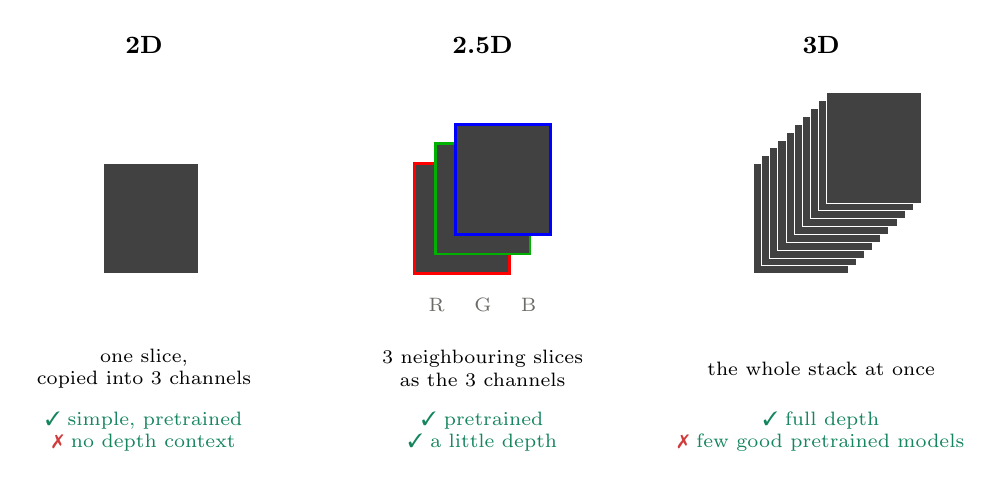
\begin{tikzpicture}[x=0.86mm,y=1mm]
  \foreach \col/\title/\txt in {0/2D/{one slice,\\ copied into 3 channels}, 50/2.5D/{3 neighbouring slices\\ as the 3 channels}, 100/3D/{the whole stack at once}} {
    \node[font=\small\bfseries] at (\col+12,29) {\title};
    \node[font=\scriptsize, align=center] at (\col+12,-12) {\txt};
  }
  % 2D
  \fill[dark!85, draw=white] (6,0) rectangle ++(14,14);
  % 2.5D
  \foreach \k/\c in {0/red,1/green!70!black,2/blue} {
    \fill[dark!85, draw=\c, line width=1pt] ({52+\k*3},{\k*2.5}) rectangle ++(14,14);
  }
  \node[font=\scriptsize, text=muted] at (62,-4) {R \quad G \quad B};
  % 3D
  \foreach \k in {0,...,9} \fill[dark!85, draw=white, line width=0.3pt] ({102+\k*1.2},{\k*1}) rectangle ++(14,14);
  % verdicts
  \node[font=\scriptsize, text=wordline, align=center] at (12,-20) {\cmark\ simple, pretrained\\ \xmark\ no depth context};
  \node[font=\scriptsize, text=wordline, align=center] at (62,-20) {\cmark\ pretrained\\ \cmark\ a little depth};
  \node[font=\scriptsize, text=wordline, align=center] at (112,-20) {\cmark\ full depth\\ \xmark\ few good pretrained models};
\end{tikzpicture}
\caption{Three ways to feed slices. We used 2.5D (8 slice triplets per series). The winners found that once
the model knows where to look, plain 2D works as well (Chapter~\ref{ch:winmodels}).}
\label{fig:25d}
\end{figure}

\section{From many slices to one answer: pooling}

A study gives many images (we used 8 triplets $\times$ 3 series = 24). Each goes through the backbone and becomes a
feature vector. They must be combined into \emph{one} prediction per study: this is \term{pooling}.

\begin{figure}[H]
\centering
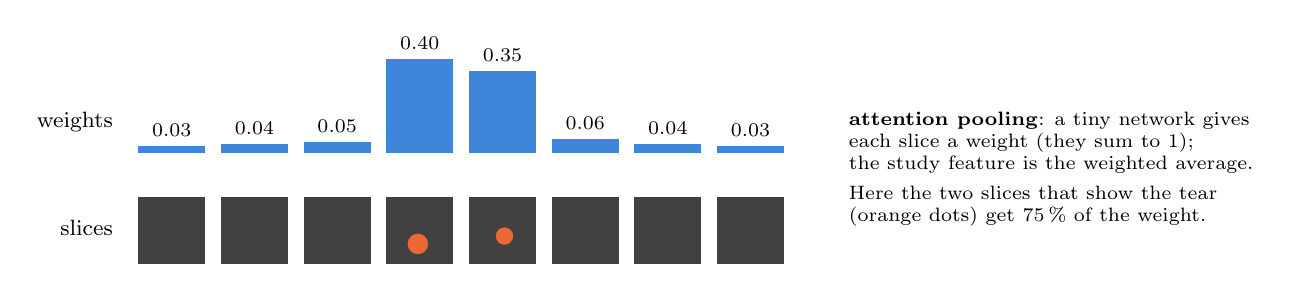
\begin{tikzpicture}[x=1mm,y=1mm]
  \foreach \k/\w in {0/0.03,1/0.04,2/0.05,3/0.40,4/0.35,5/0.06,6/0.04,7/0.03} {
    \fill[dark!85] ({\k*10.5},0) rectangle ++(8.5,8.5);
    \fill[us!90] ({\k*10.5},14) rectangle ++(8.5,{\w*30});
    \node[font=\scriptsize] at ({\k*10.5+4.25},{16+\w*30}) {\w};
  }
  \fill[them] (35.5,2.5) circle (1.3); \fill[them] (46.5,3.5) circle (1.1);
  \node[font=\footnotesize, anchor=east] at (-2,4.5) {slices};
  \node[font=\footnotesize, anchor=east] at (-2,18) {weights};
  \node[font=\scriptsize, align=left, anchor=west] at (89,12) {\textbf{attention pooling}: a tiny network gives\\
     each slice a weight (they sum to 1);\\ the study feature is the weighted average.\\[1mm]
     Here the two slices that show the tear\\ (orange dots) get 75\,\% of the weight.};
\end{tikzpicture}
\caption{A tear is visible on two or three slices out of 24. A plain average would dilute it; attention pooling lets
the model focus on the slices that matter. Because only the study has a label, not each slice, this setting is
called \term{multiple-instance learning}.}
\label{fig:attnpool}
\end{figure}

\section{From numbers to probabilities}

The head outputs 12 raw numbers called \term{logits} (any value from $-\infty$ to $+\infty$). Each one is squeezed
into a probability by the \term{sigmoid} function $\sigma(z) = 1/(1+e^{-z})$:

\begin{figure}[H]
\centering
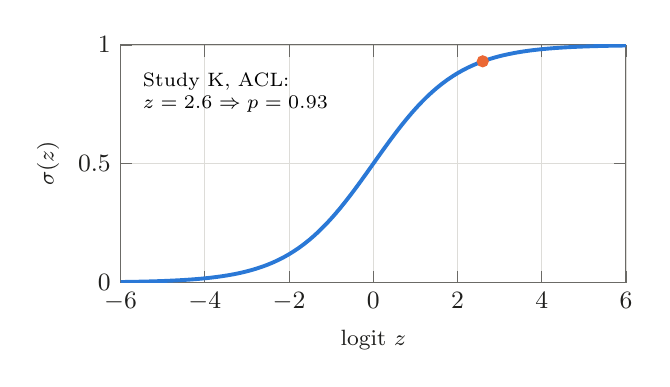
\begin{tikzpicture}
\begin{axis}[width=8cm, height=4.6cm, xmin=-6, xmax=6, ymin=0, ymax=1, xlabel={logit $z$}, ylabel={$\sigma(z)$},
    ymajorgrids, xmajorgrids, xtick={-6,-4,...,6}, ytick={0,0.5,1}, xlabel style={font=\footnotesize},
    ylabel style={font=\footnotesize}]
  \addplot[us, line width=1.4pt, domain=-6:6, samples=100] {1/(1+exp(-x))};
  \addplot[only marks, mark=*, mark size=2pt, them] coordinates {(2.6,0.931)};
  \node[font=\scriptsize, anchor=west, align=left] at (axis cs:-5.7,0.8) {Study K, ACL:\\ $z=2.6 \Rightarrow p=0.93$};
\end{axis}
\end{tikzpicture}
\caption{The sigmoid. Each of the 12 findings has its own sigmoid, so all 12 can be high at the same time (a
\emph{multi-label} model).}
\end{figure}

\section{The loss: how wrong is the model?}

Training needs one number that says how bad the current predictions are: the \term{loss}. For yes/no labels the
standard is \term{binary cross-entropy} (BCE):
\[
\text{BCE}(p, y) = -\big[\, y\log p + (1-y)\log(1-p) \,\big]
\]
where $p$ is the predicted probability and $y$ the label.

\begin{figure}[H]
\centering
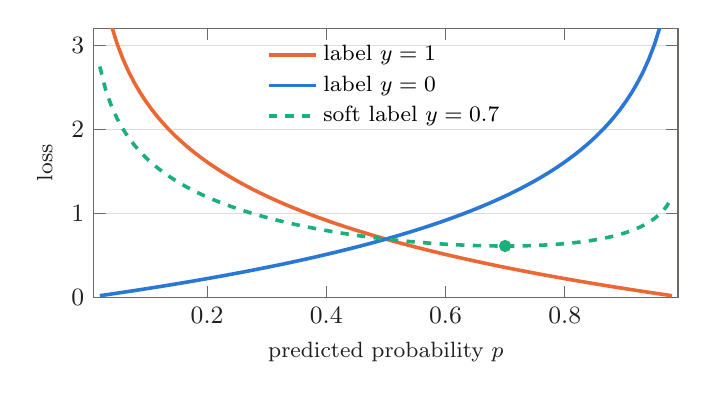
\begin{tikzpicture}
\begin{axis}[width=9cm, height=5cm, xmin=0.01, xmax=0.99, ymin=0, ymax=3.2, xlabel={predicted probability $p$},
    ylabel={loss}, ymajorgrids, xlabel style={font=\footnotesize}, ylabel style={font=\footnotesize},
    legend style={at={(0.5,0.98)}, anchor=north}]
  \addplot[them, line width=1.3pt, domain=0.02:0.98, samples=100] {-ln(x)};
  \addplot[us, line width=1.3pt, domain=0.02:0.98, samples=100] {-ln(1-x)};
  \addplot[third, line width=1.3pt, dashed, domain=0.02:0.98, samples=100] {-(0.7*ln(x)+0.3*ln(1-x))};
  \addplot[only marks, mark=*, mark size=2pt, third] coordinates {(0.7,0.611)};
  \legend{{label $y=1$}, {label $y=0$}, {soft label $y=0.7$}}
\end{axis}
\end{tikzpicture}
\caption{BCE punishes confident mistakes hard: predicting 0.02 for a true positive costs 3.9. With a
\term{soft label} such as 0.7 (``probably yes''), the loss is smallest exactly at $p=0.7$ (dot). That is how
uncertain labels from reports can be used directly.}
\label{fig:bce}
\end{figure}

\begin{keyidea}
Soft labels let the model learn ``probably yes'' instead of a forced yes or no. Both our pipeline and the
winners' trained on soft labels between 0 and 1.
\end{keyidea}

\begin{wordcheck}
\term{Masked loss}: when a label is unknown (missing), it is simply left out of the loss, so it neither rewards nor
punishes the model. Our training code did this for every missing label.
\end{wordcheck}

\section{The training loop}

\begin{figure}[H]
\centering
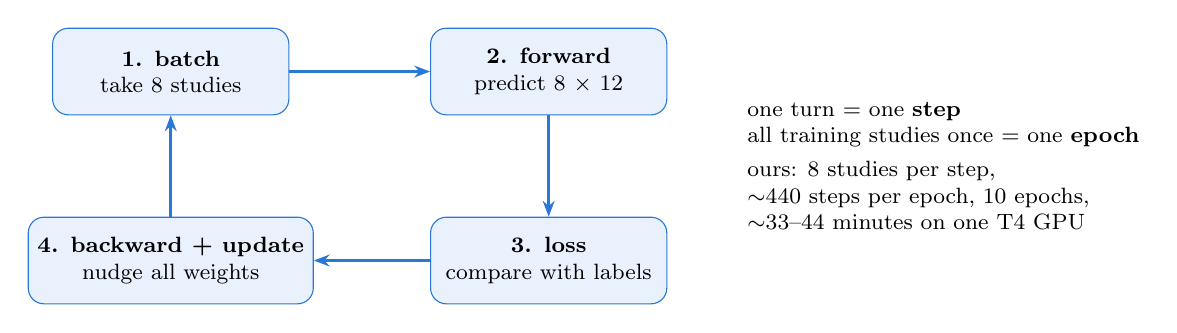
\begin{tikzpicture}[x=1mm,y=1mm,
  st/.style={draw=accent, fill=keyfill, rounded corners=2mm, minimum width=30mm, minimum height=11mm,
             align=center, font=\footnotesize},
  ar/.style={-{Stealth[length=2mm]}, line width=0.9pt, accent}]
  \node[st] (a) at (0,18) {\textbf{1. batch}\\ take 8 studies};
  \node[st] (b) at (48,18) {\textbf{2. forward}\\ predict 8 $\times$ 12};
  \node[st] (c) at (48,-6) {\textbf{3. loss}\\ compare with labels};
  \node[st] (d) at (0,-6) {\textbf{4. backward + update}\\ nudge all weights};
  \draw[ar] (a) -- (b); \draw[ar] (b) -- (c); \draw[ar] (c) -- (d); \draw[ar] (d) -- (a);
  \node[font=\footnotesize, align=left, anchor=west] at (72,6) {one turn = one \textbf{step}\\
     all training studies once = one \textbf{epoch}\\[1mm]
     ours: 8 studies per step,\\ \ca 440 steps per epoch, 10 epochs,\\ \ca 33--44 minutes on one T4 GPU};
\end{tikzpicture}
\caption{The loop. ``Backward'' computes, for every weight, which direction lowers the loss (the
\term{gradient}); the \term{optimizer} (we and the winners used \term{AdamW}) takes a small step that way.}
\end{figure}

How big a step? That is the \term{learning rate}. It usually starts small (\term{warm-up}), then decreases
smoothly (\term{cosine decay}):

\begin{figure}[H]
\centering
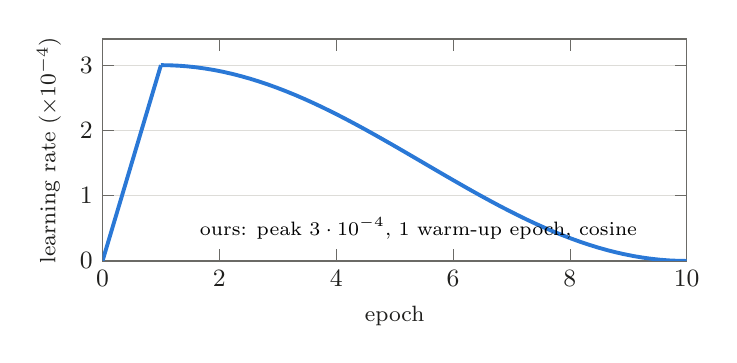
\begin{tikzpicture}
\begin{axis}[width=9cm, height=4.4cm, xmin=0, xmax=10, ymin=0, ymax=3.4, xlabel={epoch},
    ylabel={learning rate ($\times10^{-4}$)}, ymajorgrids, xlabel style={font=\footnotesize},
    ylabel style={font=\footnotesize}]
  \addplot[us, line width=1.4pt, domain=0:1, samples=20] {3*x};
  \addplot[us, line width=1.4pt, domain=1:10, samples=60] {1.5*(1+cos(deg(pi*(x-1)/9)))};
  \node[font=\scriptsize, anchor=west] at (axis cs:1.5,0.5) {ours: peak $3\cdot10^{-4}$, 1 warm-up epoch, cosine};
\end{axis}
\end{tikzpicture}
\caption{Our learning-rate schedule. The winners used a lower, constant rate for one model and a higher one with
a ``one-cycle'' schedule for another (Chapter~\ref{ch:winmodels}).}
\end{figure}

\section{Overfitting and augmentation}

A model with millions of knobs can simply \emph{memorise} its training studies. It then looks perfect on them and
poor on new ones: \term{overfitting}.

\begin{figure}[H]
\centering
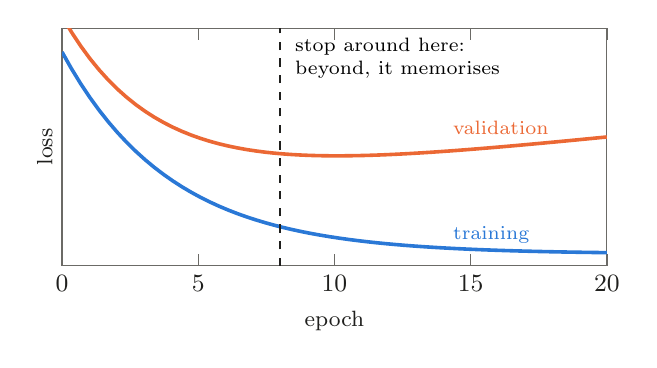
\begin{tikzpicture}
\begin{axis}[width=8.5cm, height=4.6cm, xmin=0, xmax=20, ymin=0, ymax=1, xlabel={epoch}, ylabel={loss},
    ytick=\empty, ymajorgrids, xlabel style={font=\footnotesize}, ylabel style={font=\footnotesize}]
  \addplot[us, line width=1.3pt, domain=0:20, samples=60] {0.85*exp(-x/4)+0.05};
  \addplot[them, line width=1.3pt, domain=0:20, samples=60] {0.75*exp(-x/3.5)+0.3+0.012*x};
  \draw[ink, dashed] (axis cs:8,0) -- (axis cs:8,1);
  \node[font=\scriptsize, anchor=west, text=us] at (axis cs:14,0.13) {training};
  \node[font=\scriptsize, anchor=west, text=them] at (axis cs:14,0.58) {validation};
  \node[font=\scriptsize, anchor=south west, align=left] at (axis cs:8.2,0.75) {stop around here:\\ beyond, it memorises};
\end{axis}
\end{tikzpicture}
\caption{Typical curves. Training loss keeps falling; the loss on unseen studies stops improving and rises.}
\end{figure}

\term{Augmentation} fights overfitting: every time a study is shown, it is changed a little at random, so the
model never sees exactly the same image twice.

\begin{figure}[H]
\centering
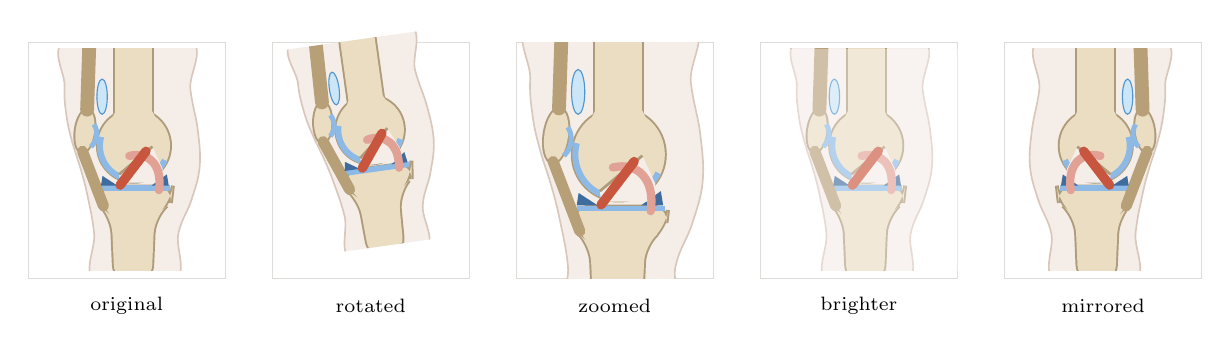
\begin{tikzpicture}
  \foreach \x/\lab in {0/original, 3.1/rotated, 6.2/zoomed, 9.3/brighter, 12.4/mirrored} {
    \node[font=\scriptsize] at (\x+1.25,-0.35) {\lab};
    \draw[grid] (\x,0) rectangle ++(2.5,3);
  }
  \begin{scope}[shift={(0.05,0.1)}, scale=0.235] \kneesagittal \end{scope}
  \begin{scope}[shift={(3.35,0.25)}, scale=0.22, rotate=8] \kneesagittal \end{scope}
  \begin{scope}[shift={(6.2,0)}] \clip (0,0) rectangle (2.5,3); \begin{scope}[shift={(-0.35,-0.45)}, scale=0.3] \kneesagittal \end{scope} \end{scope}
  \begin{scope}[shift={(9.35,0.1)}, scale=0.235] \kneesagittal \fill[white, opacity=0.35] (0,0) rectangle (10.5,12); \end{scope}
  \begin{scope}[shift={(14.85,0.1)}, xscale=-0.235, yscale=0.235] \kneesagittal \end{scope}
\end{tikzpicture}
\caption{Augmentations we used: small rotation, zoom and shift, brightness/contrast/gamma changes, and mirroring
the whole knee left--right. All are applied on the GPU, per series, at random.}
\label{fig:augment}
\end{figure}

\section{Validation: testing honestly}

To know whether a change helps, you need studies the model did not train on. \term{K-fold cross-validation}
splits the training studies into $k$ parts (\term{folds}), trains $k$ models, each with one fold held out:

\begin{figure}[H]
\centering
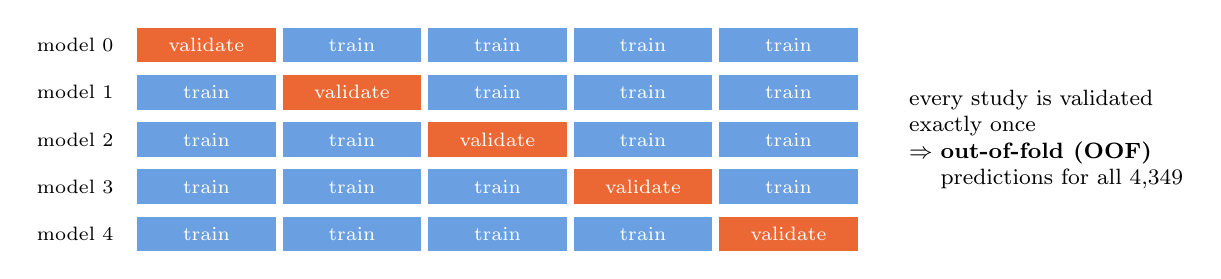
\begin{tikzpicture}[x=0.88mm,y=1mm]
  \foreach \m in {0,...,4} {
    \node[font=\scriptsize, anchor=east] at (-2,{-\m*6}) {model \m};
    \foreach \f in {0,...,4} {
      \ifnum\f=\m
        \fill[them] ({\f*21},{-\m*6-2.2}) rectangle ++(20,4.4);
        \node[font=\scriptsize, text=white] at ({\f*21+10},{-\m*6}) {validate};
      \else
        \fill[us!70] ({\f*21},{-\m*6-2.2}) rectangle ++(20,4.4);
        \node[font=\scriptsize, text=white] at ({\f*21+10},{-\m*6}) {train};
      \fi
    }
  }
  \node[font=\footnotesize, align=left, anchor=west] at (110,-12) {every study is validated\\ exactly once\\
     $\Rightarrow$ \textbf{out-of-fold (OOF)}\\ \hspace*{4mm}predictions for all 4,349};
\end{tikzpicture}
\caption{5-fold cross-validation. At submission time the 5 models are averaged (a free ensemble).}
\label{fig:kfold}
\end{figure}

\begin{watchout}
If studies from the same hospital are in both the training and the validation folds, the model can recognise the
hospital (its scanner, its image style) and the score looks better than it will be on new hospitals. We split
\textbf{by site}: all studies of one site proxy (report language + scanner vendor, 31 groups) go into the same
fold. This is called \term{GroupKFold}.
\end{watchout}

\section{Ensembles and test-time augmentation}

\begin{itemize}
\item \term{Ensemble}: average the predictions of several models. Their mistakes partly cancel. It helps most when
      the models are \emph{different} (other labels, other inputs), and very little when they are near-copies.
\item \term{Rank averaging}: AUC only cares about order, so instead of averaging probabilities you can convert each
      model's predictions to ranks (1st, 2nd, \ldots) and average those. This stops one over-confident model from
      dominating.
\item \term{Test-time augmentation} (TTA): predict on the original and on a mirrored copy, then average. We used
      mirror TTA.
\end{itemize}

\begin{innumbers}
Our EfficientNet-B0 and ConvNeXt-Nano models (one fold each, same images and labels) scored 0.886 and 0.898 on
the 58 gold studies; their rank average scored 0.903. A small but typical ensemble gain.
\end{innumbers}

\begin{checkpoint}
\begin{itemize}
\done I can draw backbone $\rightarrow$ feature vector $\rightarrow$ head and say which part is pretrained.
\done I know what 2.5D means, what pooling does, and why soft labels work with BCE.
\done I can explain k-fold and why we grouped folds by site.
\quiz Q5.1: Why use 3 neighbouring slices as the 3 channels instead of one slice copied 3 times?
\quiz Q5.2: A label is 0.5 (``don't know''). What prediction minimises its BCE, and what does the model learn from it?
\quiz Q5.3: Two models trained on the same images with the same labels and different random seeds. Will
      ensembling them help a lot? Why?
\end{itemize}
\end{checkpoint}

\chapter{Measuring success: ROC-AUC}
\label{ch:auc}

\begin{tldr}
\begin{itemize}
\item \textbf{Accuracy is useless} when positives are rare: ``always no'' scores 98\,\% on MCL.
\item \textbf{AUC} = the share of (sick, healthy) pairs that the model puts in the right order. 0.5 = random, 1 = perfect.
\item Only the \textbf{order} of the predictions matters, never their exact values.
\item With few test cases AUC is \textbf{noisy}: on our 58 gold studies, $\pm$0.02 macro is luck.
\end{itemize}
\end{tldr}

\section{Why not just count correct answers?}

\begin{example}
In our report labels, only about 2\,\% of studies have a high-grade MCL tear. A ``model'' that always answers
\emph{no} is right 98\,\% of the time. Its accuracy is excellent, and it is completely useless: it finds no tears.
\end{example}

We need a score that rewards \emph{finding the sick ones} and does not care how rare they are. That is ROC-AUC.

\section{AUC as a ranking game}

Give the model 8 studies. It returns a score for each; sort them from highest to lowest:

\begin{figure}[H]
\centering
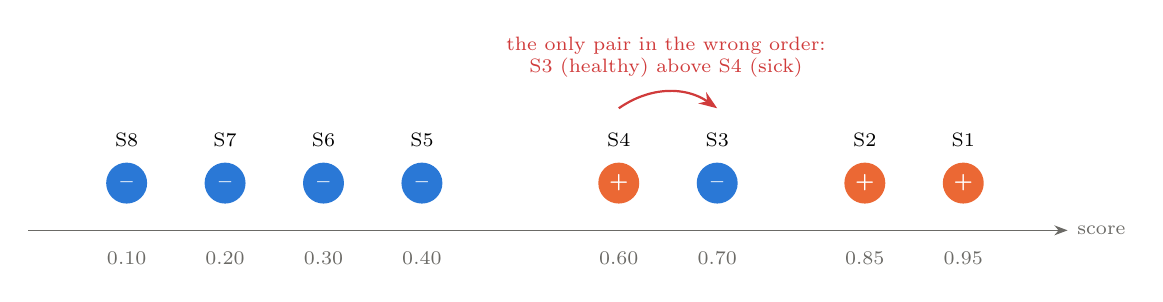
\begin{tikzpicture}[x=1mm,y=1mm]
  \draw[muted, -{Stealth}] (0,0) -- (132,0) node[right, font=\scriptsize] {score};
  \foreach \s/\p/\n in {95/1/S1, 85/1/S2, 70/0/S3, 60/1/S4, 40/0/S5, 30/0/S6, 20/0/S7, 10/0/S8} {
    \pgfmathsetmacro{\x}{\s*1.25}
    \ifnum\p=1
      \fill[them] (\x,6) circle (2.6);
      \node[font=\scriptsize\bfseries, text=white] at (\x,6) {+};
    \else
      \fill[us] (\x,6) circle (2.6);
      \node[font=\scriptsize\bfseries, text=white] at (\x,6) {--};
    \fi
    \node[font=\scriptsize] at (\x,11.5) {\n};
    \node[font=\scriptsize, text=muted] at (\x,-3.5) {0.\s};
  }
  % the one wrong pair
  \draw[warnline, line width=0.8pt, -{Stealth}] (75,15.5) to[bend left=35] (87.5,15.5);
  \node[font=\scriptsize, text=warnline, align=center] at (81,22) {the only pair in the wrong order:\\ S3 (healthy) above S4 (sick)};
\end{tikzpicture}
\caption{Eight studies on the model's score axis (higher score to the right). Orange~+ = has the finding,
blue~-- = does not.}
\label{fig:rankgame}
\end{figure}

Now form every pair of one sick and one healthy study: $3 \times 5 = 15$ pairs. Count the pairs where the sick one
has the higher score:
\begin{itemize}
\item S1 beats all 5 healthy ones: 5 \quad S2 beats all 5: 5 \quad S4 beats S5--S8 but not S3: 4.
\end{itemize}
\[
\text{AUC} = \frac{5+5+4}{15} = \frac{14}{15} = 0.933
\]

\begin{keyidea}
\textbf{AUC is the probability that a random sick study gets a higher score than a random healthy one.}
It does not depend on how rare the finding is, and it does not depend on the scores themselves, only on
their order.
\end{keyidea}

\section{The ROC curve}

The same number has a picture. Move a threshold from the top score down. At each step, count the sick studies above
the threshold (\term{true-positive rate}, TPR) and the healthy ones above it (\term{false-positive rate}, FPR):

\begin{figure}[H]
\centering
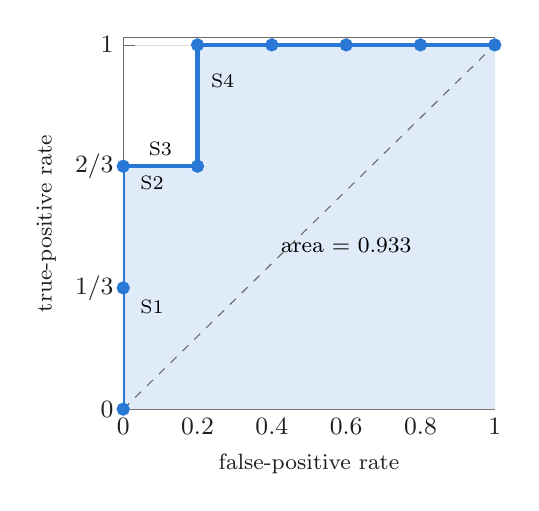
\begin{tikzpicture}
\begin{axis}[width=6.3cm, height=6.3cm, xmin=0, xmax=1, ymin=0, ymax=1.02, xlabel={false-positive rate},
    ylabel={true-positive rate}, xtick={0,0.2,...,1}, ytick={0,0.333,0.667,1}, yticklabels={0,1/3,2/3,1},
    xlabel style={font=\footnotesize}, ylabel style={font=\footnotesize}, grid=major]
  \addplot[fill=us!15, draw=none] coordinates {(0,0) (0,0.667) (0.2,0.667) (0.2,1) (1,1) (1,0)} \closedcycle;
  \addplot[us, line width=1.5pt, mark=*, mark size=1.6pt] coordinates
     {(0,0) (0,0.333) (0,0.667) (0.2,0.667) (0.2,1) (0.4,1) (0.6,1) (0.8,1) (1,1)};
  \addplot[muted, dashed] coordinates {(0,0) (1,1)};
  \node[font=\footnotesize] at (axis cs:0.6,0.45) {area = 0.933};
  \node[font=\scriptsize, anchor=west] at (axis cs:0.02,0.28) {S1};
  \node[font=\scriptsize, anchor=west] at (axis cs:0.02,0.62) {S2};
  \node[font=\scriptsize, anchor=south] at (axis cs:0.1,0.67) {S3};
  \node[font=\scriptsize, anchor=west] at (axis cs:0.21,0.9) {S4};
\end{axis}
\end{tikzpicture}\hspace{6mm}
\begin{minipage}[b]{0.42\linewidth}\small
Start at (0,0). Walk down the sorted list:
\begin{itemize}
\item a \textcolor{them}{\textbf{sick}} study: step \textbf{up} by 1/3;
\item a \textcolor{us}{\textbf{healthy}} study: step \textbf{right} by 1/5.
\end{itemize}
The area under the staircase is the AUC. A perfect model goes straight up, then right (area 1). A random model
follows the dashed diagonal (area 0.5).\par\bigskip
\end{minipage}
\caption{The ROC curve of the 8-study example. ROC = ``receiver operating characteristic'', a name from radar
engineering; AUC = ``area under the curve''.}
\end{figure}

\section{Real curves from our model}

These are the actual ROC curves of our v4 model (5 folds, EfficientNet-B0) on the 58 gold studies:

\begin{figure}[H]
\centering
\begin{tikzpicture}
\begin{axis}[width=7.2cm, height=7.2cm, xmin=0, xmax=1, ymin=0, ymax=1, xlabel={false-positive rate},
    ylabel={true-positive rate}, xlabel style={font=\footnotesize}, ylabel style={font=\footnotesize}, grid=major,
    legend style={at={(0.97,0.03)}, anchor=south east}]
  \addplot[them, line width=1.4pt, const plot] table[x=fpr, y=tpr] {figdata/roc_eff.dat};
  \addplot[us, line width=1.4pt, const plot] table[x=fpr, y=tpr] {figdata/roc_acl.dat};
  \addplot[third, line width=1.4pt, const plot] table[x=fpr, y=tpr] {figdata/roc_syn.dat};
  \addplot[muted, dashed] coordinates {(0,0) (1,1)};
  \legend{{Effusion: \auceff}, {ACL: \aucacl}, {Synovitis: \aucsyn}}
\end{axis}
\end{tikzpicture}
\caption{Effusion and ACL are found well; Synovitis is our weakest finding. With only \goldPosSyn{} synovitis
positives among the 58 studies the staircase has large steps: every single study moves the curve.}
\label{fig:realroc}
\end{figure}

\section{Twelve AUCs become one: the macro average}

\begin{figure}[H]
\centering
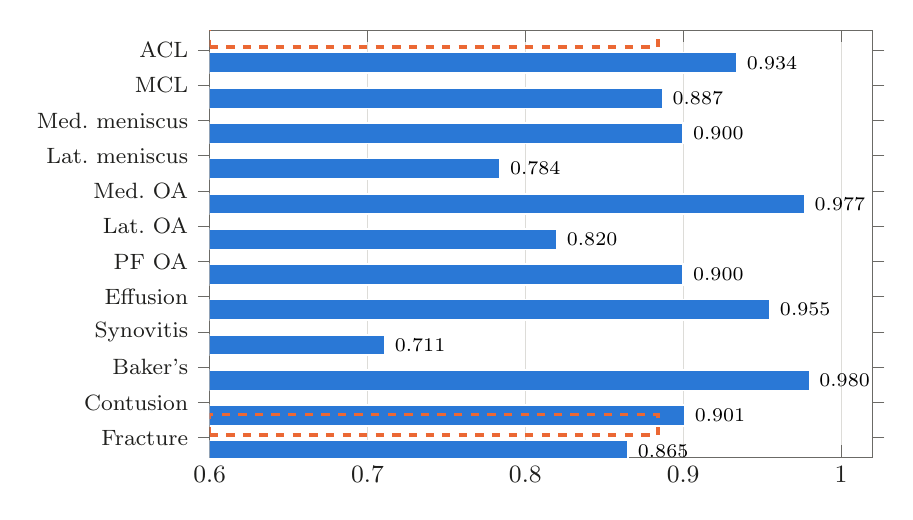
\begin{tikzpicture}
\begin{axis}[xbar, width=10cm, height=7cm, bar width=2.6mm, xmin=0.6, xmax=1.02,
    symbolic y coords={Fracture,Contusion,Baker's,Synovitis,Effusion,PF OA,Lat.~OA,Med.~OA,Lat.~meniscus,Med.~meniscus,MCL,ACL},
    ytick=data, y tick label style={font=\footnotesize}, xtick={0.6,0.7,0.8,0.9,1.0},
    xmajorgrids, nodes near coords, nodes near coords style={font=\scriptsize, anchor=west},
    point meta=explicit symbolic, enlarge y limits=0.05]
  \addplot[barus] coordinates {(0.934,ACL) [0.934] (0.887,MCL) [0.887] (0.900,Med.~meniscus) [0.900]
     (0.784,Lat.~meniscus) [0.784] (0.977,Med.~OA) [0.977] (0.820,Lat.~OA) [0.820] (0.900,PF OA) [0.900]
     (0.955,Effusion) [0.955] (0.711,Synovitis) [0.711] (0.980,Baker's) [0.980] (0.901,Contusion) [0.901]
     (0.865,Fracture) [0.865]};
  \addplot[them, line width=1.2pt, dashed, nodes near coords={}] coordinates {(0.884,Fracture) [] (0.884,ACL) []};
\end{axis}
\end{tikzpicture}
\caption{Our v4 model on the 58 gold studies, per finding. The dashed line is the macro average, \goldMacro.
Synovitis, Lateral meniscus and Lateral OA pull it down most.}
\label{fig:perfinding}
\end{figure}

\begin{why}
The competition uses the \emph{macro} average (each finding counts 1/12) so that a model cannot ignore the rare
findings. Improving Synovitis from 0.71 to 0.81 lifts the score by $0.10/12 \approx 0.008$, as much as improving every
finding by 0.008.
\end{why}

\section{Only the order matters}

Because AUC only looks at the order of scores:
\begin{itemize}
\item multiplying all predictions by 10, squaring them or passing them through any increasing function changes
      nothing;
\item a model can be badly \emph{calibrated} (its 0.8 does not mean ``80\,\% chance'') and still have a perfect AUC;
\item to combine models, you can average their \textbf{ranks} instead of their probabilities (Chapter~\ref{ch:submission}).
\end{itemize}

\begin{watchout}
Calibration does not matter for the \emph{score}, but it matters for \emph{training labels}. A label of 0.98 that
should be 0.6 teaches the model to be confidently wrong. The winners judged their labels on calibration too
(Chapter~\ref{ch:winlabels}).
\end{watchout}

\section{How noisy is an AUC?}

\begin{figure}[H]
\centering
\begin{tikzpicture}
\begin{axis}[ybar interval, width=10cm, height=4.8cm, xmin=0.82, xmax=0.94, ymin=0, ymax=330, xlabel={macro AUC on a resampled gold set},
    ytick=\empty, axis y line=none, axis x line*=bottom, xlabel style={font=\footnotesize},
    xtick={0.82,0.84,...,0.94}, xticklabel style={/pgf/number format/fixed, /pgf/number format/precision=2}]
  \addplot[fill=us!70, draw=white] table[x=left, y=n] {figdata/gold_bootstrap.dat};
  \draw[them, line width=1.4pt] (axis cs:0.884,0) -- (axis cs:0.884,300);
  \node[font=\scriptsize, text=them!85!black, anchor=west] at (axis cs:0.886,290) {measured: \goldMacro};
\end{axis}
\end{tikzpicture}
\caption{The same predictions, scored on 2,000 random resamples of the 58 gold studies (a \term{bootstrap}). The
middle 90\,\% of the results spans \bootLo--\bootHi. A difference of 0.01 between two models on gold tells you almost
nothing.}
\label{fig:bootstrap}
\end{figure}

\begin{innumbers}
\begin{itemize}
\item 58 gold studies: macro AUC uncertain by about $\pm$0.02; a single finding by $\pm$0.05 to $\pm$0.09 (MCL has only
      9 positives).
\item Public leaderboard (\ca 390 studies): about $\pm$0.005.
\item Out-of-fold predictions on 4,349 report-labelled studies: much more stable, but measured against
      \emph{our own} labels, which have their own errors.
\end{itemize}
\end{innumbers}

\begin{keyidea}
Every score is measured against \emph{something}: the 58 gold labels (trustworthy but few), report labels (many
but noisy) or the public leaderboard (hidden, limited submissions). Use them together and be suspicious of small
differences. The winners spent real effort choosing their ruler (Chapter~\ref{ch:winmodels}).
\end{keyidea}

\begin{checkpoint}
\begin{itemize}
\done I can compute an AUC by counting pairs.
\done I can draw a ROC curve from a sorted list.
\done I know why a 0.01 gain on 58 gold studies is not evidence.
\quiz Q6.1: A model outputs 0.51 for every sick study and 0.49 for every healthy one. What is its AUC?
\quiz Q6.2: You add 0.3 to every prediction of one finding. What happens to the AUC?
\quiz Q6.3: Which matters more for the final score: raising Baker's from 0.98 to 0.99, or Synovitis from 0.71 to
      0.75?
\end{itemize}
\end{checkpoint}


\part{What we built}
\chapter{Step 1: reports into labels}
\label{ch:labels}
\whereami{2}

\begin{tldr}
\begin{itemize}
\item We used an open \textbf{large language model} (LLM), running inside Kaggle, to read all 4,407 reports.
\item \textbf{v3} (Qwen2.5-7B) asked for one word per finding and used ``any grade counts'': agreement with the
      doctors' gold labels \textbf{0.809} AUC.
\item \textbf{v4} (Qwen2.5-32B) used the organisers' thresholds, five answer letters, and read the model's
      \textbf{probabilities} instead of its text: \textbf{0.879}. Leaderboard of the image model: 0.889 $\rightarrow$ 0.905.
\item Reports cannot label what they do not mention: \textbf{Synovitis} is silent in 84\,\% of them.
\end{itemize}
\end{tldr}

\section{What a language model does}

A language model reads text split into \term{tokens} (word pieces) and, at every position, outputs a probability
for every possible next token. Generating text means picking a token, appending it and repeating.

\begin{figure}[H]
\centering
\begin{tikzpicture}[x=1mm,y=1mm]
  \node[draw=grid, fill=white, rounded corners=1.5mm, text width=56mm, font=\scriptsize\ttfamily, align=left,
        inner sep=2mm] (p) at (0,0) {[instructions: 12 findings, definitions, letters P M U A N]\\[1mm]
        [report of Study K]\\[1mm] \{"ACL": "};
  \node[draw=accent, fill=keyfill, rounded corners=2mm, minimum width=20mm, minimum height=12mm, font=\footnotesize,
        align=center] (m) at (50,0) {\faRobot\\ LLM};
  \draw[-{Stealth}, muted, line width=0.8pt] (p) -- (m);
  \foreach \t/\v [count=\i from 0] in {P/0.95, M/0.02, U/0.02, A/0.01, N/0.00, {the}/0.00} {
    \node[font=\scriptsize\ttfamily, anchor=east] at (72,{9-\i*3.6}) {\t};
    \fill[grid] (73,{9-\i*3.6-1.1}) rectangle ++(40,2.2);
    \fill[us] (73,{9-\i*3.6-1.1}) rectangle ++({40*\v},2.2);
    \node[font=\scriptsize, anchor=west] at (114,{9-\i*3.6}) {\v};
  }
  \draw[-{Stealth}, muted, line width=0.8pt] (m) -- (66,0);
  \node[font=\scriptsize, text=muted, align=center] at (93,-15) {probability of each possible next token\\ (the full vocabulary has \ca 150,000)};
\end{tikzpicture}
\caption{The prompt ends right where the answer for ACL should start. The model's next-token probabilities
\emph{are} the answer: 95\,\% ``P'' (present, past the threshold).}
\label{fig:nexttoken}
\end{figure}

\begin{wordcheck}
\term{LLM}: large language model, e.g.\ ChatGPT, Claude, Qwen. \term{Open-weights model}: one whose weights you can
download and run yourself (Qwen is made by Alibaba). \term{Prompt}: the text you give the model.
\term{4-bit quantization}: storing each weight in 4 bits instead of 16 so a big model fits in less memory.
\end{wordcheck}

\section{Why an open model, inside Kaggle?}

We believed the competition's data rules forbade sending report text to hosted services such as ChatGPT or
Claude, so the reports never left Kaggle. A Kaggle notebook offers two T4 GPUs with 16\,GB each, for at most
12 hours per session. A 32-billion-parameter model only fits in 4-bit form (19\,GB spread over both GPUs).

\begin{watchout}
That belief was \textbf{wrong}. The organisers had stated in a pinned forum post that hosted LLM APIs, including
for labelling reports, were allowed. We never read that post. The winners used the strongest hosted models and,
crucially, let them look at the images too (Chapter~\ref{ch:winlabels}). Lesson: \textbf{check the rules threads on
day one, and treat every self-imposed rule as a question to verify.}
\end{watchout}

\section{Version 3: the first labeller}

\begin{center}\small
\begin{tabularx}{\linewidth}{l>{\raggedright\arraybackslash}X}
\toprule
Model & Qwen2.5-7B-Instruct (16-bit) \\
Prompt & ``for each finding, answer \code{present}, \code{minimal}, \code{uncertain}, \code{absent} or \code{not\_mentioned}; any grade counts'' \\
Reading the answer & parse the generated text; map to label values 1, 0.5 or 0 \\
Runtime & 3.8 hours for 4,407 reports; 3.6\,\% of reports had an unparseable answer \\
Agreement with gold & \textbf{macro AUC 0.809} \\
\bottomrule
\end{tabularx}
\end{center}

Two problems showed up when we compared it with the 58 gold studies:
\begin{enumerate}
\item \textbf{Wrong definitions.} ``Any grade counts'' turned every small effusion and every mild sprain into a
      positive. The organisers' rule is the opposite (Figure~\ref{fig:thresholds}).
\item \textbf{Silence became ``absent''.} The model almost never answered \code{not\_mentioned} (0--2 of 58 gold
      reports per finding). But ``the report does not mention synovitis'' is not the same as ``no synovitis''.
\end{enumerate}

\section{Version 4: four changes}

\subsection*{1. The organisers' thresholds, written into the prompt}

For every finding the prompt lists what counts as \textbf{P} (present and past the threshold) and what counts as
\textbf{M} (present but below it). Two examples:

\begin{center}\small
\begin{tabularx}{\linewidth}{l>{\raggedright\arraybackslash}X>{\raggedright\arraybackslash}X}
\toprule
 & P (counts) & M (does not count) \\
\midrule
Effusion & moderate or large joint effusion & small, trace, minimal, mild or physiological fluid \\
MCL & acute high-grade partial or complete tear (grade 2--3) & grade 1 sprain, edema around an intact ligament, old scarring \\
\bottomrule
\end{tabularx}
\end{center}

\subsection*{2. Five answers instead of three}

\begin{figure}[H]
\centering
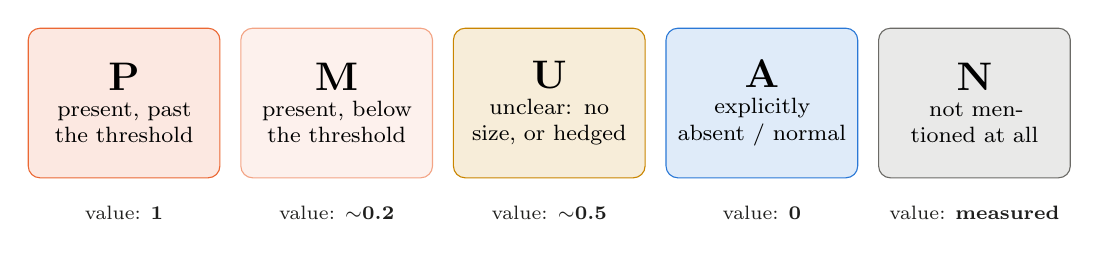
\begin{tikzpicture}[x=1mm,y=1mm,
  let/.style={draw=#1, fill=#1!15, rounded corners=1.5mm, minimum width=24mm, minimum height=19mm, align=center,
              font=\footnotesize, text width=22mm}]
  \node[let=them] at (0,0) {\textbf{\Large P}\\ present, past the threshold};
  \colorlet{mcol}{them!60}
  \node[let=mcol] at (27,0) {\textbf{\Large M}\\ present, below the threshold};
  \node[let=whyline] at (54,0) {\textbf{\Large U}\\ unclear: no size, or hedged};
  \node[let=us] at (81,0) {\textbf{\Large A}\\ explicitly absent / normal};
  \node[let=muted] at (108,0) {\textbf{\Large N}\\ not mentioned at all};
  \foreach \x/\v in {0/1, 27/{\ca 0.2}, 54/{\ca 0.5}, 81/0, 108/{measured}} {
    \node[font=\scriptsize, text=ink] at (\x,-14) {value: \textbf{\v}};
  }
\end{tikzpicture}
\caption{The five answer letters and their label values. The values for M, U and N were measured on the gold
studies per finding (how often a gold doctor said ``positive'' after that answer), pulled towards the defaults
shown here so that 58 studies do not overrule common sense.}
\label{fig:letters}
\end{figure}

\begin{example}
``Not mentioned'' means different things for different findings. For \textbf{Fracture} a silent report almost
always means no fracture (value \ca 0). For \textbf{Synovitis}, 15 of the 41 gold studies whose report was silent
were positive, so N gets a value of about \textbf{0.33}: ``we don't know, but a third of these knees have it''.
\end{example}

\subsection*{3. Read probabilities instead of text}

\begin{figure}[H]
\centering
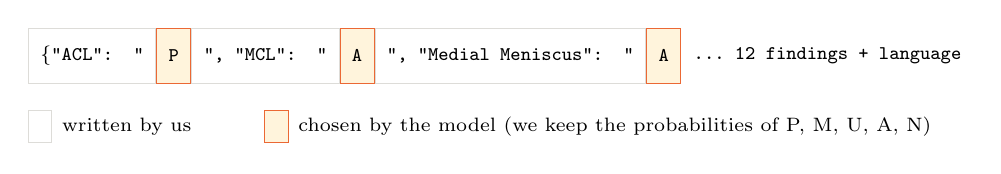
\begin{tikzpicture}[x=1mm,y=1mm,
  seg/.style={draw=grid, fill=white, font=\scriptsize\ttfamily, minimum height=7mm, inner sep=1.5mm},
  ans/.style={draw=them, fill=whyfill, font=\scriptsize\ttfamily\bfseries, minimum height=7mm, inner sep=1.5mm}]
  \node[seg, anchor=west] (a) at (0,0) {\{"ACL": "};
  \node[ans, anchor=west] (b) at (a.east) {P};
  \node[seg, anchor=west] (c) at (b.east) {", "MCL": "};
  \node[ans, anchor=west] (d) at (c.east) {A};
  \node[seg, anchor=west] (e) at (d.east) {", "Medial Meniscus": "};
  \node[ans, anchor=west] (f) at (e.east) {A};
  \node[seg, anchor=west, draw=none] (g) at (f.east) {\ldots\ 12 findings + language};
  \node[seg, anchor=west, minimum height=4mm] (k1) at (0,-9) {};
  \node[font=\scriptsize, anchor=west] at (k1.east) {written by us};
  \node[ans, anchor=west, minimum height=4mm] (k2) at (30,-9) {};
  \node[font=\scriptsize, anchor=west] at (k2.east) {chosen by the model (we keep the probabilities of P, M, U, A, N)};
\end{tikzpicture}
\caption{We wrote the JSON answer ourselves and let the model fill in only the letters. At each gap we kept the
probabilities of all five letters (Figure~\ref{fig:nexttoken}). 13 tiny model calls per report instead of
\ca 110 generated tokens, and no parsing errors.}
\label{fig:prefill}
\end{figure}

The soft label is the probability-weighted value:
\[
\text{label} = \sum_{\text{letter}} p(\text{letter}) \cdot \text{value}(\text{letter})
\]

\begin{example}
Study K, ACL: $p$(P) = 0.95, $p$(M) = 0.02, $p$(U) = 0.02, $p$(A) = 0.01, $p$(N) = 0.00. \\
Label $= 0.95\cdot1 + 0.02\cdot0.2 + 0.02\cdot0.5 + 0.01\cdot0 = \mathbf{0.964}$. \\
Study K, Synovitis: $p$(N) = 0.97 $\Rightarrow$ label $\approx 0.97 \cdot 0.33 \approx \mathbf{0.32}$: ``unknown, prior
about one in three''.
\end{example}

\subsection*{4. A bigger model, made affordable}

\begin{figure}[H]
\centering
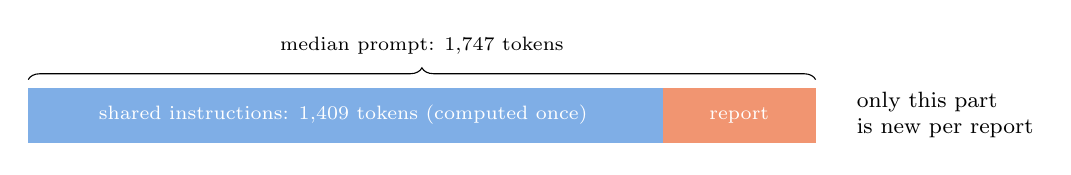
\begin{tikzpicture}[x=1mm,y=1mm]
  \fill[us!60] (0,0) rectangle (80.6,7);
  \node[font=\scriptsize, text=white] at (40,3.5) {shared instructions: 1,409 tokens (computed once)};
  \fill[them!70] (80.6,0) rectangle (100,7);
  \node[font=\scriptsize, text=white] at (90.3,3.5) {report};
  \draw[decorate, decoration={brace, amplitude=1.5mm}] (0,8) -- (100,8) node[midway, above=2mm, font=\scriptsize]
      {median prompt: 1,747 tokens};
  \node[font=\footnotesize, align=left, anchor=west] at (104,3.5) {only this part\\ is new per report};
\end{tikzpicture}
\caption{81\,\% of every prompt is the same instructions. Their internal state (the \term{KV cache}) was computed
once and reused for every report, which made the 32B model affordable on two T4s.}
\end{figure}

\paragraph{Safety rails.} Self-tests at start-up (the shortcut gives the same numbers as the plain model); the
58 gold reports first, and the 4,407-report run only if their macro AUC reached 0.84 (a \term{gate}); a time
limit of 10.5\,h with resume, because Kaggle kills sessions at 12\,h and a killed run saves nothing.

\section{Results}

\begin{figure}[H]
\centering
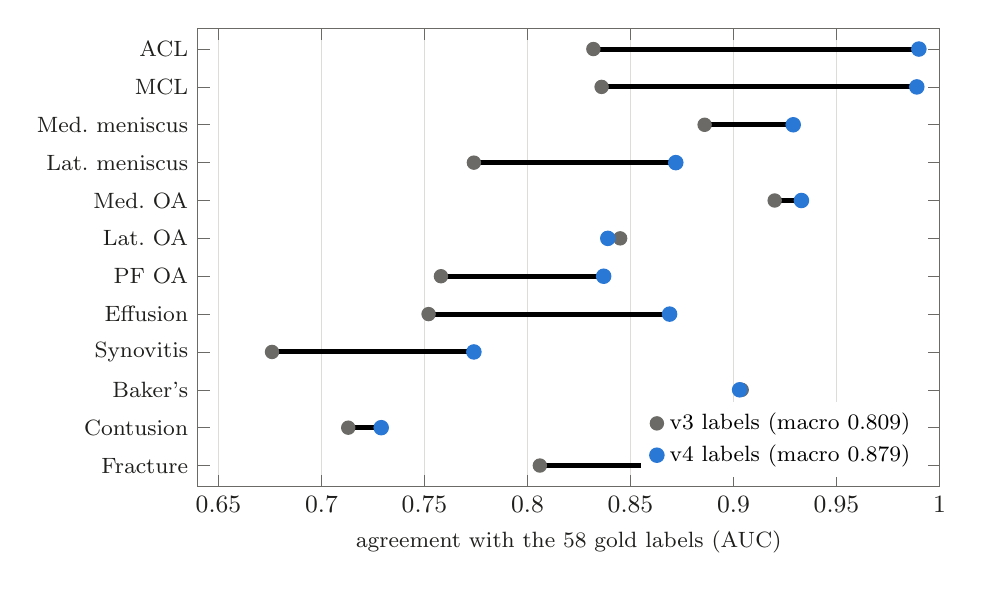
\begin{tikzpicture}
\begin{axis}[width=11cm, height=7.4cm, xmin=0.64, xmax=1.0,
    symbolic y coords={Fracture,Contusion,Baker's,Synovitis,Effusion,PF OA,Lat.~OA,Med.~OA,Lat.~meniscus,Med.~meniscus,MCL,ACL},
    ytick=data, y tick label style={font=\footnotesize}, xmajorgrids, xlabel={agreement with the 58 gold labels (AUC)},
    xlabel style={font=\footnotesize}, enlarge y limits=0.05, legend style={at={(0.98,0.02)}, anchor=south east, fill=white}]
  \addplot[grid, line width=1.8pt, forget plot] coordinates {(0.832,ACL) (0.99,ACL)};
  \addplot[grid, line width=1.8pt, forget plot] coordinates {(0.836,MCL) (0.989,MCL)};
  \addplot[grid, line width=1.8pt, forget plot] coordinates {(0.886,Med.~meniscus) (0.929,Med.~meniscus)};
  \addplot[grid, line width=1.8pt, forget plot] coordinates {(0.774,Lat.~meniscus) (0.872,Lat.~meniscus)};
  \addplot[grid, line width=1.8pt, forget plot] coordinates {(0.92,Med.~OA) (0.933,Med.~OA)};
  \addplot[grid, line width=1.8pt, forget plot] coordinates {(0.845,Lat.~OA) (0.839,Lat.~OA)};
  \addplot[grid, line width=1.8pt, forget plot] coordinates {(0.758,PF OA) (0.837,PF OA)};
  \addplot[grid, line width=1.8pt, forget plot] coordinates {(0.752,Effusion) (0.869,Effusion)};
  \addplot[grid, line width=1.8pt, forget plot] coordinates {(0.676,Synovitis) (0.774,Synovitis)};
  \addplot[grid, line width=1.8pt, forget plot] coordinates {(0.904,Baker's) (0.903,Baker's)};
  \addplot[grid, line width=1.8pt, forget plot] coordinates {(0.713,Contusion) (0.729,Contusion)};
  \addplot[grid, line width=1.8pt, forget plot] coordinates {(0.806,Fracture) (0.886,Fracture)};
  \addplot[only marks, mark=*, mark size=2.4pt, color=muted] coordinates {
    (0.832,ACL) (0.836,MCL) (0.886,Med.~meniscus) (0.774,Lat.~meniscus) (0.920,Med.~OA) (0.845,Lat.~OA)
    (0.758,PF OA) (0.752,Effusion) (0.676,Synovitis) (0.904,Baker's) (0.713,Contusion) (0.806,Fracture)};
  \addplot[only marks, mark=*, mark size=2.6pt, color=us] coordinates {
    (0.990,ACL) (0.989,MCL) (0.929,Med.~meniscus) (0.872,Lat.~meniscus) (0.933,Med.~OA) (0.839,Lat.~OA)
    (0.837,PF OA) (0.869,Effusion) (0.774,Synovitis) (0.903,Baker's) (0.729,Contusion) (0.886,Fracture)};
  \legend{{v3 labels (macro 0.809)}, {v4 labels (macro 0.879)}}
\end{axis}
\end{tikzpicture}
\caption{How well each label set agrees with the doctors, per finding. The threshold-aware v4 fixed ACL and MCL
(almost perfect: reports state ligament tears clearly), and helped effusion, fracture and PF OA. Synovitis and
contusion stayed weak.}
\label{fig:v3v4}
\end{figure}

\begin{innumbers}
Same image model, only the labels changed: \textbf{0.889 $\rightarrow$ 0.905} on the public leaderboard. On gold, the
model's ACL went 0.887 $\rightarrow$ 0.934, MCL 0.810 $\rightarrow$ 0.887, PF OA 0.799 $\rightarrow$ 0.900. The
biggest single gain of our whole project.
\end{innumbers}

\section{What the labeller actually answered}

\begin{figure}[H]
\centering
\begin{tikzpicture}
\begin{axis}[width=8.2cm, height=9cm, enlargelimits=false, colormap={bl}{color=(white) color=(us)},
    xtick={0,...,4}, xticklabels={P,M,U,A,N}, x tick label style={font=\footnotesize\bfseries},
    ytick={0,...,11}, yticklabels={ACL,MCL,Med.\ meniscus,Lat.\ meniscus,Med.\ OA,Lat.\ OA,PF OA,Effusion,Synovitis,Baker's,Contusion,Fracture},
    y tick label style={font=\footnotesize}, y dir=reverse, axis line style={draw=none}, tick style={draw=none},
    nodes near coords={\pgfmathprintnumber[fixed, precision=0]{\pgfplotspointmeta}}, nodes near coords style={font=\scriptsize, anchor=center},
    point meta min=0, point meta max=100, xticklabel pos=top]
  \addplot[matrix plot*, mesh/cols=5, point meta=explicit] table[x=x, y=y, meta=share] {figdata/letters.dat};
\end{axis}
\end{tikzpicture}
\caption{The labeller's most likely letter for each finding, in \% of the 4,349 report-only studies. Synovitis is
``not mentioned'' (N) in \synSilent\,\% of reports. MCL is P in only 1.4\,\% (the threshold wording was too strict:
6 of the 9 gold-positive MCL studies were answered M).}
\label{fig:letterheat}
\end{figure}

\begin{figure}[H]
\centering
\begin{tikzpicture}
\begin{axis}[ybar interval, width=10cm, height=4.6cm, xmin=0, xmax=1, ymin=0, xlabel={soft label for Effusion},
    ylabel={studies}, xlabel style={font=\footnotesize}, ylabel style={font=\footnotesize}, ymajorgrids,
    xtick={0,0.2,...,1}, xticklabel style={/pgf/number format/fixed}]
  \addplot[fill=us!70, draw=white] table[x=left, y=n] {figdata/effusion_hist.dat};
\end{axis}
\end{tikzpicture}
\caption{What the v4 labels look like for Effusion. Three peaks: clearly no (0, 38\,\%), clearly yes (1, 22\,\%), and
a large group at \textbf{0.44}: reports that mention an effusion without saying how much (answer U). The value of
U for Effusion, measured on the gold studies, is 0.44: a bit less than half of such knees had a moderate or large
effusion, so 0.44 is the honest label. Soft-label training
(Figure~\ref{fig:bce}) uses these in-between values directly.}
\end{figure}

\section{What reports cannot do}

\begin{keyidea}
A report-based label can only be as good as the report. Where reports are explicit (ACL, MCL) our labels reached
0.99. Where they are silent or vague (Synovitis, Contusion, Lateral OA) no prompt could fix it: \textbf{the
information is in the images, not in the text.} This is exactly where the winners' approach (reading the images
as well) made the difference.
\end{keyidea}

\begin{checkpoint}
\begin{itemize}
\done I can explain the five letters and how a soft label is computed from them.
\done I know why reading probabilities beats parsing generated text.
\done I know which findings reports label well and which they cannot.
\quiz Q7.1: Why is ``not mentioned'' not the same as ``absent''? Give a finding where the difference is large.
\quiz Q7.2: v4 labels improved ACL from 0.83 to 0.99 agreement. Why did the image model's gold ACL only go from
      0.89 to 0.93?
\quiz Q7.3: What does the ``gate'' protect against?
\end{itemize}
\end{checkpoint}

\chapter{Step 2: images into a cache}
\label{ch:cache}
\whereami{3}

\begin{tldr}
\begin{itemize}
\item Reading DICOM files is slow, so we did it \textbf{once} and saved every study as three small 3D arrays: the
      \textbf{cache}.
\item Per study: pick 3 series (sagittal, coronal, axial, fluid-sensitive), \textbf{sort} the slices,
      \textbf{rotate/flip} them to one convention, \textbf{normalise} brightness, \textbf{crop} 140\,mm around the knee,
      \textbf{resize} to 24 slices of 256\,$\times$\,256 pixels.
\item The same Python file prepares the hidden test images inside the submission, so training and test images are
      made \textbf{identically}.
\end{itemize}
\end{tldr}

\section{Why a cache?}

Training reads every study 10 times per model, and we trained 5 models per experiment. Decoding hundreds of thousands of
DICOM files each time would take hours. Decoding once (\ca 1.5--2 hours of CPU) and saving compact arrays makes every
later experiment fast.

\begin{figure}[H]
\centering
\begin{tikzpicture}[x=0.95mm,y=1mm,
  st/.style={draw=accent, fill=keyfill, rounded corners=1.5mm, minimum width=20mm, minimum height=13mm,
             align=center, font=\scriptsize, text width=19mm},
  ar/.style={-{Stealth[length=1.6mm]}, line width=0.7pt, accent}]
  \foreach \i/\t in {0/{\textbf{a} pick\\ 3 series}, 1/{\textbf{b} sort\\ slices}, 2/{\textbf{c} same\\ orientation},
                     3/{\textbf{d} note\\ left/right}, 4/{\textbf{e} normalise\\ brightness}, 5/{\textbf{f} crop\\ the knee},
                     6/{\textbf{g} resize\\ 24$\times$256$\times$256}} {
    \node[st] (n\i) at ({\i*22.5},0) {\t};
  }
  \foreach \i [evaluate=\i as \j using int(\i+1)] in {0,...,5} \draw[ar] (n\i) -- (n\j);
  \node[font=\scriptsize, text=muted] at (0,-11) {\faFolder\ DICOM files};
  \node[font=\scriptsize, text=muted] at (135,-11) {\faCube\ 3 arrays per study};
\end{tikzpicture}
\caption{The seven steps, applied to every study. The code lives in one file, \code{knee\_preproc.py}, saved together
with the cache.}
\label{fig:cacheflow}
\end{figure}

\section{a. Pick one series per role}

A study has about 5.5 series. We keep three \term{roles}: \code{sag\_fs}, \code{cor\_fs}, \code{ax\_fs} (sagittal,
coronal, axial; fluid-sensitive). \code{train\_series.csv} says what each series is; a small score picks the best:

\begin{figure}[H]
\centering
\begin{tikzpicture}[x=1mm,y=1mm,
  ser/.style={draw=grid, fill=white, rounded corners=1mm, minimum width=34mm, minimum height=8mm, font=\scriptsize,
              align=left, anchor=west},
  win/.style={ser, draw=us, line width=0.9pt, fill=keyfill}]
  \node[ser] at (0,20) {Sagittal, fluid, fat-sat \hfill \textbf{7}};
  \node[ser] at (0,10) {Sagittal, T1 \hfill 1};
  \node[ser] at (0,0)  {Coronal, fluid, fat-sat \hfill \textbf{7}};
  \node[ser] at (0,-10) {Coronal, T1 \hfill 1};
  \node[ser] at (0,-20) {Axial, fluid, fat-sat \hfill \textbf{7}};
  \node[win] (r1) at (70,20) {\code{sag\_fs}};
  \node[win] (r2) at (70,0) {\code{cor\_fs}};
  \node[win] (r3) at (70,-20) {\code{ax\_fs}};
  \foreach \y in {20,0,-20} \draw[-{Stealth}, us, line width=0.8pt] (35,\y) -- (69,\y);
  \node[font=\scriptsize, align=left, anchor=west] at (108,0) {score =\\ \hspace*{2mm}4 if fluid-sensitive\\
     \hspace*{2mm}+ 2 if also fat-suppressed\\ \hspace*{2mm}+ 1 if 12--80 slices\\[1mm] highest score wins;\\
     no fluid series in a plane:\\ take any (``fallback'')};
\end{tikzpicture}
\caption{Series selection for one study. All three roles were available in 100\,\% of training studies.}
\end{figure}

\section{b. Sort the slices}

File names are random IDs. The only reliable order is the physical one: project each slice's
\code{ImagePositionPatient} onto the slice direction and sort by that number.

\begin{figure}[H]
\centering
\begin{tikzpicture}[x=1mm,y=1mm]
  \foreach \k/\o in {0/3,1/0,2/5,3/1,4/4,5/2} {
    \pgfmathsetmacro{\g}{35+\o*9}
    \fill[dark!\g] ({\k*9},0) rectangle ++(7,10);
    \node[font=\tiny] at ({\k*9+3.5},-2.5) {\o};
  }
  \node[font=\scriptsize, align=center] at (25,-8) {sorted by file name: jumbled};
  \draw[-{Stealth}, line width=1pt, muted] (58,5) -- (72,5);
  \foreach \k in {0,...,5} {
    \pgfmathsetmacro{\g}{35+\k*9}
    \fill[dark!\g] ({78+\k*9},0) rectangle ++(7,10);
    \node[font=\tiny] at ({78+\k*9+3.5},-2.5) {\k};
  }
  \node[font=\scriptsize, align=center] at (103,-8) {sorted by position (mm): correct};
\end{tikzpicture}
\caption{Wrong slice order turns a 3D stack into noise for anything that looks at neighbouring slices.}
\end{figure}

\section{c. One orientation for everybody}

Sites store the same plane in different ways: rotated, mirrored, upside down. The header's
\code{ImageOrientationPatient} says how, so every series can be flipped or transposed into one convention (for
sagittal: front of the knee on the left, head at the top).

\begin{figure}[H]
\centering
\begin{tikzpicture}
  \foreach \x/\lab in {0/{site A}, 2.3/{site B}, 4.6/{site C}, 6.9/{site D}} {
    \draw[grid] (\x,0) rectangle ++(2,2.3);
    \node[font=\scriptsize] at (\x+1,-0.3) {\lab};
  }
  \begin{scope}[shift={(0.05,0.05)}, scale=0.19] \kneesagittal \end{scope}
  \begin{scope}[shift={(4.25,0.05)}, xscale=-0.19, yscale=0.19] \kneesagittal \end{scope}
  \begin{scope}[shift={(4.65,2.25)}, xscale=0.19, yscale=-0.19] \kneesagittal \end{scope}
  \begin{scope}[shift={(8.9,0.28)}, rotate=90, scale=0.165] \kneesagittal \end{scope}
  \draw[-{Stealth}, line width=1pt, muted] (9.3,1.15) -- (10.6,1.15);
  \draw[accent, line width=1pt] (11,0) rectangle ++(2,2.3);
  \begin{scope}[shift={(11.05,0.05)}, scale=0.19] \kneesagittal \end{scope}
  \node[font=\scriptsize\bfseries, text=accent] at (12,-0.3) {canonical};
\end{tikzpicture}
\caption{Four ways the same sagittal image can be stored, and the one convention every series is turned into. We
checked that five real storage variants of one series produced identical output.}
\end{figure}

\section{d. Left or right knee: written down, not changed}

For a right knee the medial side is towards the patient's left, for a left knee the other way. The cache keeps the
patient's own orientation and records the \code{Laterality} tag (present in 49.8\,\% of studies) so a later step can
mirror left knees if wanted. We tried that in Chapter~\ref{ch:experiments} (``v7'').

\section{e. Normalise the brightness}

\begin{figure}[H]
\centering
\begin{tikzpicture}
\begin{axis}[width=10cm, height=4.6cm, xmin=0, xmax=3000, ymin=0, ymax=1.15, ytick=\empty, axis y line=none,
    axis x line*=bottom, xlabel={raw pixel value of one series}, xlabel style={font=\footnotesize},
    xticklabel style={font=\scriptsize}, scaled x ticks=false]
  \addplot[fill=us!25, draw=us, domain=0:3000, samples=150] {1.0*exp(-((x-40)/45)^2) + 0.45*exp(-((x-700)/220)^2) + 0.25*exp(-((x-1400)/260)^2) + 0.03*exp(-((x-2600)/200)^2)} \closedcycle;
  \draw[them, line width=1.2pt, dashed] (axis cs:15,0) -- (axis cs:15,1.1) node[above, font=\scriptsize] {0.5\,\%};
  \draw[them, line width=1.2pt, dashed] (axis cs:2150,0) -- (axis cs:2150,1.1) node[above, font=\scriptsize] {99.5\,\%};
  \node[font=\scriptsize, align=left, anchor=west] at (axis cs:120,0.8) {air (background)};
  \node[font=\scriptsize, align=center] at (axis cs:1050,0.6) {tissue};
  \node[font=\scriptsize, align=center] at (axis cs:2600,0.3) {rare bright\\ outliers};
\end{axis}
\end{tikzpicture}
\caption{Per series: find the 0.5th and 99.5th percentile, map that range to 0--255, clip the rest. Outliers no longer
decide the contrast, and every series ends up on the same scale (compare Chapter~\ref{ch:mri}).}
\end{figure}

\section{f. Crop the knee}

The field of view varies between sites (often 150--200\,mm), and much of it is thigh and shin. We found the knee
automatically and cut a fixed square around it:

\begin{figure}[H]
\centering
\begin{tikzpicture}[scale=0.5]
  \fill[black] (-1.5,-1.0) rectangle (11.5,13.0);
  \begin{scope}[shift={(0,0)}]
    \clip (-1.5,-1.0) rectangle (11.5,13.0);
    \kneecoronal
  \end{scope}
  \draw[us, line width=1.6pt, dashed] (0.5,0.5) rectangle (9.5,9.5);
  \node[font=\scriptsize\bfseries, text=us, fill=white, inner sep=1pt, anchor=south west] at (0.5,9.6) {140\,mm (v5)};
  \draw[them, line width=1.6pt] (2.1,2.3) rectangle (7.9,8.1);
  \node[font=\scriptsize\bfseries, text=them, fill=white, inner sep=1pt, anchor=north west] at (2.1,2.2) {90\,mm (v8)};
  \node[font=\scriptsize\bfseries, text=white, anchor=north west] at (-1.4,12.9) {full field of view, e.g.\ 200\,mm};
\end{tikzpicture}\hspace{6mm}
\begin{minipage}[b]{0.42\linewidth}\small
\textbf{How the knee is found:}
\begin{enumerate}
\item average all slices of the series into one image;
\item ``tissue'' = pixels brighter than 30\,\% of the 99th percentile;
\item the tissue box = rows and columns that are at least 5\,\% tissue;
\item centre a 140\,mm square on that box (pad with black if the image is smaller).
\end{enumerate}
We stored how much tissue fell outside (\code{tissue\_outside}) to check that no knee was cut.\par\medskip
\end{minipage}
\caption{The crop window. The bigger the window, the less detail per millimetre after resizing to 256 pixels.}
\label{fig:crop}
\end{figure}

\section{g. Resize to one shape}

Every series becomes exactly \textbf{24 slices of 256\,$\times$\,256 pixels}, stored as 8-bit integers (0--255):
linear interpolation between slices, smooth (anti-aliased) resizing within a slice.

\begin{center}\footnotesize
\begin{tabular}{lllll}
\toprule
Cache & Window & Pixels & mm/pixel & Result (Chapter~\ref{ch:experiments}) \\
\midrule
first (v1--v4) & whole field of view & 224 & \ca 0.7--0.9 & 0.905 public \\
\textbf{v5} & 140\,mm around the knee & 256 & 0.55 & \textbf{0.918} public \\
v6 & 130\,mm & 320 & 0.41 & +0.002--0.004 val.: stopped \\
v8 & 90\,mm on the joint & 256 & 0.35 & prepared; result not recorded \\
\midrule
\textcolor{them}{winners} & 140\,mm; 112\,mm on the joint & 384--512 & 0.27--0.36 & 0.960 private \\
\bottomrule
\end{tabular}
\end{center}

\begin{innumbers}
One study = 3 roles $\times$ 24 $\times$ 256 $\times$ 256 bytes $\approx$ 4.7\,MB, so the whole training set is
\ca 21\,GB in memory. Kaggle notebooks may output at most 500 files and 20\,GB, so the cache was written as
\textbf{45 compressed shards} of 100 studies each.
\end{innumbers}

\section{The same code at test time}

\begin{keyidea}
The submission notebook imports the \emph{same} \code{knee\_preproc.py} from the cache dataset and runs it on the
hidden test DICOMs. Any difference between training and test preparation (another resize method, another
orientation rule) would silently cost score, and you would never see why.
\end{keyidea}

\begin{watchout}
24 slices per series is a compromise. Native series have 20--40 slices; resampling to 24 blurs thin structures
across slices. The winners kept up to 64 \emph{native} slices and higher in-plane resolution, and used five series
instead of three. That costs much more GPU time, which on Kaggle's free T4s we did not have.
\end{watchout}

\begin{checkpoint}
\begin{itemize}
\done I can list the seven preparation steps and say why each is needed.
\done I know why the cache module is reused in the submission.
\quiz Q8.1: Why normalise each series separately instead of the whole dataset at once?
\quiz Q8.2: Cropping from 200\,mm to 140\,mm and keeping 256 pixels: how much finer does each pixel get?
\quiz Q8.3: The cache does not mirror left knees. What would go wrong if it mirrored only the sagittal series?
\end{itemize}
\end{checkpoint}

\chapter{Step 3: the model}
\label{ch:model}
\whereami{4}

\begin{tldr}
\begin{itemize}
\item Our model (\code{KneeNet}): each of the 3 series gives \textbf{8 slice triplets}; one shared \textbf{EfficientNet-B0}
      turns each triplet into a feature vector; \textbf{attention pooling} makes one vector per series; a small
      \textbf{MLP} turns the three vectors into 12 outputs.
\item Trained on \textbf{soft labels} with a masked BCE loss, \textbf{10 epochs}, about \textbf{44 minutes per fold} on one T4.
\item Kaggle's GPUs taught us three hard rules: \textbf{T4 not P100}, \textbf{one GPU per process}, \textbf{fp16 not bf16}.
\end{itemize}
\end{tldr}

\section{The architecture}

\begin{figure}[H]
\centering
\begin{tikzpicture}[x=0.86mm,y=1mm,
  lab/.style={font=\scriptsize, align=center},
  ar/.style={-{Stealth[length=1.6mm]}, line width=0.6pt, muted}]
  % three series
  \foreach \r/\name/\y in {0/sag/22, 1/cor/0, 2/ax/-22} {
    \foreach \k in {0,...,4} \fill[dark!85, draw=white, line width=0.3pt] ({\k*1},{\y-6+\k*0.8}) rectangle ++(10,10);
    \node[lab, anchor=east] at (-1.5,\y) {\code{\name\_fs}\\ 24 slices};
    % triplets
    \foreach \t in {0,...,7} {
      \fill[red!60] ({21+\t*4.2},{\y-3}) rectangle ++(3.2,6);
      \fill[green!50!black!60] ({21.4+\t*4.2},{\y-3.4}) rectangle ++(3.2,6);
      \fill[blue!60] ({21.8+\t*4.2},{\y-3.8}) rectangle ++(3.2,6);
    }
    \draw[ar] (16,\y) -- (20,\y);
    % backbone
    \draw[ar] (56,\y) -- (60,\y);
    % features
    \foreach \t in {0,...,7} \fill[us!70] ({80+\t*1.6},{\y-4}) rectangle ++(1.2,8);
    \draw[ar] (76,\y) -- (79,\y);
    % attention pool -> one vector
    \node[draw=us, fill=keyfill, rounded corners=1mm, lab, minimum width=13mm, minimum height=8mm] (ap\r) at (102,\y) {attention\\ pool};
    \draw[ar] (93,\y) -- (ap\r.west);
    \fill[us] (113,{\y-4}) rectangle ++(2,8);
    \draw[ar] (ap\r.east) -- (112.5,\y);
    \node[lab, anchor=west] at (116,\y) {+ role\\ embedding};
  }
  \node[draw=accent, fill=keyfill, rounded corners=2mm, minimum width=15mm, minimum height=60mm, lab] (bb) at (68,0)
       {\textbf{shared}\\ \textbf{EfficientNet-B0}\\[1mm] same weights\\ for all\\ 24 images};
  \node[lab] at (36,34) {8 triplets per series\\ (3 slices = R, G, B)};
  \node[lab] at (86,34) {8 feature vectors\\ (1,280 numbers each)};
  % concat and head
  \node[draw=them, fill=whyfill, rounded corners=1.5mm, lab, minimum width=19mm, minimum height=14mm] (head) at (156,0)
       {concatenate\\ + MLP head};
  \foreach \y in {22,0,-22} \draw[ar] (132,\y) -- (head.west);
  \foreach \k in {0,...,11} \fill[them!80] ({151+\k*0.9},-14) rectangle ++(0.7,3);
  \node[lab] at (156,-18) {12 logits};
  \draw[ar] (head) -- (156,-10.5);
\end{tikzpicture}
\caption{\code{KneeNet}. 3 series $\times$ 8 triplets = 24 images per study go through the same backbone; pooling and the
head then reduce them to 12 numbers. With a batch of 8 studies, the backbone sees 192 images per step.}
\label{fig:kneenet}
\end{figure}

\subsection*{Slice triplets}

From the 24 cached slices we pick 8 evenly spaced centres (slice 1, 4, 7, \ldots, 22). Each centre plus its two
neighbours becomes one 3-channel image, exactly the shape an ImageNet backbone expects (Figure~\ref{fig:25d}).
During training every centre moves by $-1$, 0 or $+1$ at random, a cheap form of augmentation.

\subsection*{Attention pooling, role embedding, mask}

\begin{itemize}
\item \textbf{Attention pooling} (Figure~\ref{fig:attnpool}): a two-layer mini-network scores each of the 8 triplet
      features; the softmax of the scores gives the weights; the weighted sum is the series feature.
\item \textbf{Role embedding}: a learned vector added to the series feature, so the head knows which feature came
      from which plane.
\item \textbf{Role mask}: if a series is missing, its feature is set to zero and a 0/1 flag tells the head. (In
      practice all three were almost always present.)
\end{itemize}

\subsection*{The head}

\begin{center}\small
\code{Dropout(0.3) $\rightarrow$ Linear(3$\times$1280 + 3 $\rightarrow$ 512) $\rightarrow$ GELU $\rightarrow$ Dropout(0.2) $\rightarrow$ Linear(512 $\rightarrow$ 12)}
\end{center}
\term{Dropout} switches off a random share of the numbers during training, another defence against
memorising.

\section{Loss and labels}

\begin{itemize}
\item Targets: the v4 soft labels (Chapter~\ref{ch:labels}), one value between 0 and 1 per finding.
\item Loss: binary cross-entropy on soft labels, with missing labels masked out (Figure~\ref{fig:bce}).
\item The \textbf{58 gold studies are never trained on}. They are predicted by the 5 fold models together and used
      only as an outside check.
\end{itemize}

\section{Augmentation, on the GPU}

All augmentation runs on the GPU, per series, so the CPU never slows training down:
\begin{itemize}
\item small rotation ($\pm$10\textdegree), zoom ($\pm$10\,\%) and shift ($\pm$5\,\%);
\item brightness, contrast and gamma changes;
\item \textbf{joint knee mirror}, with probability 0.5:
\end{itemize}

\begin{figure}[H]
\centering
\begin{tikzpicture}[x=1mm,y=1mm]
  \node[font=\footnotesize\bfseries] at (20,30) {original knee};
  \node[font=\footnotesize\bfseries] at (95,30) {mirrored knee (all three together)};
  \foreach \x/\m in {0/0, 75/1} {
    % sagittal: slice order
    \foreach \k in {0,...,5} {
      \pgfmathsetmacro{\g}{\m==0 ? 30+\k*10 : 80-\k*10}
      \fill[dark!\g] ({\x+\k*4},14) rectangle ++(3,10);
    }
    \node[font=\scriptsize, anchor=west] at ({\x+26},19) {sagittal: slice order};
    % coronal and axial: left-right flip
    \fill[dark!80] (\x,0) rectangle ++(22,10);
    \fill[them] ({\x+(\m==0 ? 3 : 15)},3) rectangle ++(4,4);
    \node[font=\scriptsize, anchor=west] at ({\x+26},5) {coronal + axial: left $\leftrightarrow$ right};
  }
  \draw[-{Stealth}, line width=1pt, muted] (58,12) -- (70,12);
\end{tikzpicture}
\caption{A mirrored knee looks like the other leg. Sagittal slices are reversed in order; coronal and axial images
are flipped. Doing it to only one series would create an impossible knee.}
\label{fig:mirror}
\end{figure}

\begin{why}
Mirroring makes the model see twice as many ``different'' knees. The price: the model can no longer tell a left
knee from a right one, and therefore medial from lateral by position alone. We tested whether that hurt in
Chapter~\ref{ch:experiments} (it did not).
\end{why}

\section{Training settings}

\begin{center}\small
\begin{tabularx}{\linewidth}{l>{\raggedright\arraybackslash}X}
\toprule
Backbone & EfficientNet-B0, ImageNet-pretrained (later also ConvNeXt-Nano) \\
Optimizer & AdamW, learning rate $3\cdot10^{-4}$, weight decay $10^{-2}$ \\
Schedule & 1 warm-up epoch, then cosine decay; 10 epochs \\
Batch & 8 studies = 192 triplet images \\
Precision & fp16 mixed precision, \code{channels\_last} memory layout \\
Data loading & 224\,px: whole cache preloaded into RAM (15.9\,GB of \ca 32\,GB); 256\,px: unpacked once to local disk and memory-mapped \\
Validation & 5-fold GroupKFold by site (31 groups); mirror TTA \\
Speed (one T4) & 224\,px: 0.41\,s/step, 33\,min/fold. 256\,px: 0.53\,s/step, 44\,min/fold \\
\bottomrule
\end{tabularx}
\end{center}

\begin{figure}[H]
\centering
\begin{tikzpicture}[x=1mm,y=1mm]
  \draw[muted] (0,0) -- (120,0);
  \foreach \t in {0,30,60,90,120} {\draw[muted] (\t,-1) -- (\t,1); \node[font=\scriptsize, below] at (\t,-1) {\pgfmathparse{int(\t)}\pgfmathresult\ min};}
  \node[font=\scriptsize, anchor=east] at (-2,14) {GPU 1};
  \node[font=\scriptsize, anchor=east] at (-2,6) {GPU 2};
  \fill[us!70] (0,11.5) rectangle (44,16.5); \node[font=\scriptsize, text=white] at (22,14) {B0 fold 0};
  \fill[us!70] (45,11.5) rectangle (89,16.5); \node[font=\scriptsize, text=white] at (67,14) {B0 fold 1};
  \fill[them!80] (0,3.5) rectangle (62,8.5); \node[font=\scriptsize, text=white] at (31,6) {ConvNeXt-Nano fold 0};
  \fill[them!80] (63,3.5) rectangle (125,8.5); \node[font=\scriptsize, text=white] at (94,6) {ConvNeXt-Nano fold 1};
\end{tikzpicture}
\caption{Our training notebook ran \emph{jobs} as separate processes, one per GPU, so both T4s were busy.}
\end{figure}

\section{Three hard rules from Kaggle's GPUs}

\begin{watchout}
\begin{enumerate}
\item \textbf{Use the T4, not the P100.} Current PyTorch no longer ships code for the P100's older architecture.
\item \textbf{One GPU per process, no \code{nn.DataParallel}.} Splitting batches across two T4s made a step 18$\times$
      slower (7.5\,s instead of 0.4\,s) and crashed the kernel. A 5-minute speed diagnostic found it after two blind
      fixes had failed. \textbf{Measure before fixing.}
\item \textbf{fp16, not bf16.} The T4 has no fast bf16 hardware; bf16 ran about 3$\times$ slower.
\end{enumerate}
\end{watchout}

\begin{innumbers}
Kaggle gives about 30 GPU hours per week and kills sessions after 12 hours (a killed run saves nothing). One
5-fold training run of B0 at 256\,px costs about 3.7 GPU hours. The budget, not ideas, set the pace of the project.
\end{innumbers}

\section{First results of the 256\,px model}

\begin{center}\small
\begin{tabular}{lccc}
\toprule
Fold 0, 256\,px, 140\,mm crop & validation AUC (903 studies) & gold AUC (58) & time per fold \\
\midrule
EfficientNet-B0 & 0.861 & 0.886 & 44 min \\
ConvNeXt-Nano & 0.857 & 0.898 & 62 min \\
rank average of the two & -- & \textbf{0.903} & \\
\bottomrule
\end{tabular}
\end{center}

Validation AUC compares with our own report labels (rounded at 0.5), gold AUC with the doctors. They disagree about
which backbone is better: with this much noise (Figure~\ref{fig:bootstrap}) neither number alone decides.

\begin{checkpoint}
\begin{itemize}
\done I can draw \code{KneeNet} from series to 12 outputs.
\done I know why mirroring must flip all three series together.
\done I know the three GPU rules and why they exist.
\quiz Q9.1: How many images does the backbone process for one batch of 8 studies?
\quiz Q9.2: Why is the gold set predicted by all 5 fold models, while each training study gets one out-of-fold
      prediction?
\quiz Q9.3: B0 is better on validation, ConvNeXt-Nano on gold. Which would you keep?
\end{itemize}
\end{checkpoint}

\chapter{Step 4: the submission}
\label{ch:submission}
\whereami{5}

\begin{tldr}
\begin{itemize}
\item The submission notebook runs \textbf{offline} on hidden data: everything it needs is attached as datasets.
\item \textbf{Safety net first}: write a valid answer file before doing anything risky, then improve it.
\item Each test study is prepared by the \textbf{same} \code{knee\_preproc.py}, predicted by every attached model
      group (with mirror TTA), and the groups are \textbf{rank-blended}.
\item To use a public notebook, we wrote a ``member cell'' that blends our ranks into its predictions.
\end{itemize}
\end{tldr}

\section{The flow}

\begin{figure}[H]
\centering
\begin{tikzpicture}[x=0.9mm,y=1mm,
  st/.style={draw=accent, fill=keyfill, rounded corners=1.5mm, minimum height=12mm, align=center,
             font=\scriptsize, text width=24mm},
  ar/.style={-{Stealth[length=1.8mm]}, line width=0.7pt, accent}]
  \node[st, draw=wordline, fill=wordfill] (a) at (0,0) {\textbf{1. safety net}\\ write a valid\\ {\ttfamily\tiny submission.csv}};
  \node[st] (b) at (30,0) {\textbf{2. offline installs}\\ JPEG decoders\\ from attached wheels};
  \node[st] (c) at (60,0) {\textbf{3. load}\\ {\ttfamily\tiny knee\_preproc.py}\\ + model groups};
  \node[st] (d) at (95,8) {\textbf{4a. prepare}\\ 32 studies\\ (4 CPU workers)};
  \node[st] (e) at (95,-12) {\textbf{4b. predict}\\ every group,\\ normal + mirrored};
  \node[st, draw=wordline, fill=wordfill] (f) at (130,-2) {\textbf{5. rewrite}\\ {\ttfamily\tiny submission.csv}\\ every few chunks};
  \draw[ar] (a) -- (b); \draw[ar] (b) -- (c); \draw[ar] (c) -- (d.west);
  \draw[ar] (d) -- (e); \draw[ar] (e.east) -- (f);
  \draw[ar, dashed] (f.north) |- (d.east) node[pos=0.75, above, font=\scriptsize] {next chunk};
\end{tikzpicture}
\caption{The submission notebook. Steps 4a--5 repeat until all \ca 1,300 test studies are done or the time limit
approaches.}
\end{figure}

\section{Safety net first}

\begin{keyidea}
A code competition punishes crashes harshly: a crash means no score, discovered hours later. So the first thing the
notebook does is write a complete, valid answer file (one guess per finding, the training prevalence). Every study is
then processed inside its own \code{try/except}; a study that fails keeps its guess, and the run goes on.
\end{keyidea}

\begin{watchout}
Two of our runs of the public-notebook version failed only because a stray one-line cell (containing the text
\code{[code]}, a paste accident) sat before our cell. A failed commit run means a failed scoring run, but you only
learn that \ca 6 hours later. \textbf{Check the cell list before you submit.}
\end{watchout}

\section{Offline installs}

Some sites store their DICOM pixels compressed (JPEG Lossless, JPEG 2000). Decoding them needs extra Python packages,
and the scoring run has no internet. We downloaded the packages' installation files (\term{wheels}) once into a Kaggle
dataset, \code{knee-dicom-wheels}, and the notebook installs them from there.

\section{Model groups and rank blending}

Every attached model dataset that contains a \code{train\_config.json} is one \term{group} (for example ``v5 B0'',
``v5 ConvNeXt-Nano''). Within a group, the 5 fold models and the 2 views (normal + mirrored) are averaged. Between
groups, predictions are combined \textbf{by rank}, per finding:

\begin{figure}[H]
\centering
\begin{tikzpicture}[x=1mm,y=1mm]
  \matrix[matrix of nodes, nodes={font=\footnotesize, minimum width=17mm, minimum height=6mm, anchor=center},
          column 1/.style={nodes={font=\footnotesize\bfseries}}, row 1/.style={nodes={font=\scriptsize\bfseries, text=muted}}] (m) {
    study & model 1 & model 2 & \textcolor{muted}{prob.\ avg.} & rank 1 & rank 2 & \textbf{rank avg.} \\
    A & 0.95 & 0.52 & 0.735 & 4 & 3 & \textbf{3.5} \\
    B & 0.10 & 0.55 & 0.325 & 2 & 4 & \textbf{3.0} \\
    C & 0.40 & 0.50 & 0.450 & 3 & 2 & \textbf{2.5} \\
    D & 0.05 & 0.49 & 0.270 & 1 & 1 & \textbf{1.0} \\
  };
  \draw[grid] (m.north west) ++(0,-7) -- ++(119,0);
  \node[font=\scriptsize, text=warnline, align=left, anchor=west] at (m.south west) [yshift=-6mm]
    {probability average: order A, C, B, D = model 1's order; the cautious model 2 is ignored};
  \node[font=\scriptsize, text=wordline, align=left, anchor=west] at (m.south west) [yshift=-11mm]
    {rank average: order A, B, C, D; both models count equally};
\end{tikzpicture}
\caption{Why rank blending. Model 2 is cautious (all its predictions are close to 0.5), so averaging probabilities lets
model 1 decide alone. Ranks put both on the same scale. Since AUC only cares about order, nothing is lost.}
\label{fig:rankblend}
\end{figure}

\code{BLEND\_WEIGHTS} can give a group a different weight per finding (for example, weight 0 for the older v3 group on
ACL, MCL and PF OA, where its labels were known to be bad).

\section{Plugging into a public notebook: the ``member cell''}

By early October the public leaderboard was crowded at \ca 0.94 by copies (\term{forks}) of one public notebook that
ran several strong published models (Chapter~\ref{ch:experiments}). We forked it and added one cell of our own:

\begin{figure}[H]
\centering
\begin{tikzpicture}[x=1mm,y=1mm,
  cell/.style={draw=grid, fill=white, rounded corners=1mm, minimum width=36mm, minimum height=8mm, font=\scriptsize,
               align=center},
  ours/.style={cell, draw=us, fill=keyfill, line width=0.9pt}]
  \node[cell] (c1) at (0,24) {public cells: their models};
  \node[cell] (c2) at (0,12) {staged predictions (ranks)};
  \node[ours, minimum height=14mm, text width=34mm] (c3) at (0,-3) {\textbf{our member cell}\\ back up $\cdot$ run our\\ models $\cdot$ blend ranks};
  \node[cell] (c4) at (0,-19) {publish \code{submission.csv}};
  \draw[-{Stealth}, muted] (c1) -- (c2); \draw[-{Stealth}, muted] (c2) -- (c3); \draw[-{Stealth}, muted] (c3) -- (c4);
  \node[font=\scriptsize, align=left, anchor=west] at (24,6) {new rank $= (1-w)\cdot$ public rank $+\ w\cdot$ our rank\\[1mm]
     $w$ = \code{OUR\_WEIGHT}, we tried 0, 0.25 and 0.4};
  \node[font=\scriptsize, align=left, anchor=west, text=warnline] at (24,-6) {any error or time-out: restore the backup,\\
     so the public result is never lost};
\end{tikzpicture}
\caption{The member cell sits just before the public notebook's final ``publish'' cell. It only touches the staged
prediction file and restores it if anything goes wrong.}
\label{fig:member}
\end{figure}

\begin{innumbers}
\begin{itemize}
\item A commit run of our own notebook (3 sample studies) took about 1--8 minutes, mostly loading models.
\item Scoring a submission of the public notebook took \ca 6 hours before the result (or an error) appeared.
\item Our member cell had a time limit (1.5--2 hours, or 20 minutes before the public notebook's own budget).
\end{itemize}
\end{innumbers}

\begin{checkpoint}
\begin{itemize}
\done I can explain the safety-net pattern and why every study gets its own \code{try/except}.
\done I can rank-blend two models by hand.
\quiz Q10.1: Why must the test images be prepared with exactly the training cache's code?
\quiz Q10.2: Two models disagree completely on one finding. What does the rank average look like?
\quiz Q10.3: What does the member cell do if our models crash halfway?
\end{itemize}
\end{checkpoint}

\chapter{Everything we tried}
\label{ch:experiments}
\whereami{6}

\begin{tldr}
\begin{itemize}
\item Own pipeline: \textbf{0.882 $\rightarrow$ 0.889 $\rightarrow$ 0.905 $\rightarrow$ 0.918} on the public leaderboard. The two
      real jumps came from \textbf{better labels} (v4) and \textbf{cropping the knee} (v5).
\item A forked public notebook scored \textbf{0.943}; adding our models to it never helped.
\item Higher resolution (320\,px) and a canonical knee side gave \textbf{nothing measurable}; we stopped each after one
      fold, by rules written in advance.
\item Final result: \textbf{0.927 private}, rank \textbf{2,968 of 6,425}. The winners: 0.960.
\end{itemize}
\end{tldr}

\section{The scoreboard}

\begin{figure}[H]
\centering
\begin{tikzpicture}
\begin{axis}[width=\linewidth, height=7.2cm, ymin=0.868, ymax=0.982, xmin=0.5, xmax=10.5,
    xtick={1,...,10}, xticklabels={v3\\4 folds, v3\\5 folds, v4, v3+v4, fork, {fork +\\v4 0.25}, {fork +\\v4 0.4},
    v5 own, {fork +\\v5 0.25}, {fork +\\v5 0.4}}, x tick label style={font=\scriptsize, align=center},
    ylabel={public leaderboard AUC}, ylabel style={font=\footnotesize}, ymajorgrids,
    yticklabel style={/pgf/number format/fixed, /pgf/number format/precision=2},
    legend style={at={(0.02,0.98)}, anchor=north west}]
  \addplot[us, line width=1.2pt, mark=*, mark size=2.4pt, nodes near coords, point meta=y,
     nodes near coords align={below}, every node near coord/.append style={font=\scriptsize, text=us!85!black,
     /pgf/number format/fixed, /pgf/number format/precision=3, /pgf/number format/fixed zerofill}]
     coordinates {(1,0.882) (2,0.889) (3,0.905) (4,0.906) (8,0.918)};
  \addplot[them, only marks, mark=square*, mark size=2.4pt, nodes near coords, point meta=y,
     nodes near coords align={above}, every node near coord/.append style={font=\scriptsize, text=them!85!black,
     /pgf/number format/fixed, /pgf/number format/precision=3, /pgf/number format/fixed zerofill}]
     coordinates {(5,0.943) (6,0.943) (7,0.936) (9,0.943) (10,0.939)};
  \addplot[muted, dashed, domain=0.5:10.5] {0.969};
  \node[font=\scriptsize, anchor=south east, text=muted] at (axis cs:10.4,0.969) {winners: 0.969 public};
  \legend{{our own pipeline}, {public notebook (+ our models)}}
\end{axis}
\end{tikzpicture}
\caption{Every scored submission we recorded, in order. Public leaderboard, so differences below \ca 0.005 are noise.}
\label{fig:scoreboard}
\end{figure}

\newcommand{\experiment}[6]{%
  \begin{tcolorbox}[enhanced, colback=white, colframe=#6, boxrule=0.6pt, leftrule=2.2mm, arc=1.2mm,
     title={#1}, fonttitle=\bfseries\small, coltitle=ink, colbacktitle=#6!12, left=3mm, right=3mm, top=1.4mm,
     bottom=1.4mm, fontupper=\small, before skip=0.8em, after skip=0.8em]
  \textbf{Idea.} #2\par\smallskip
  \textbf{What we did.} #3\par\smallskip
  \textbf{Result.} #4\par\smallskip
  \textbf{Verdict.} #5
  \end{tcolorbox}}

\section{Experiment by experiment}

\experiment{E1 \quad Baseline: v3 labels, whole knee, EfficientNet-B0}
  {Get a complete, working pipeline end to end before improving anything.}
  {v3 labels (Chapter~\ref{ch:labels}); whole field of view resized to 24\,$\times$\,224\,$\times$\,224; the
   \code{KneeNet} of Chapter~\ref{ch:model}; 4, then 5 folds.}
  {\textbf{0.882} (4 folds) and \textbf{0.889} (5 folds) public; gold macro 0.876.}
  {Works. Next question: where is it weak, and why?}{muted}

\experiment{E2 \quad Detective work: compare model and labels per finding}
  {If the model is only as good as its labels on some findings, better labels are the lever there.}
  {Scored the labels themselves against the 58 gold studies and put them next to the model's gold AUC, per finding.
   Compared with numbers that other teams published for hosted-LLM labels.}
  {On ACL, MCL, PF OA and the menisci the model sat at the level of its labels, and those labels were 0.07--0.19 below
   what a strong labeller reached. On Effusion, Contusion, Fracture and Baker's the model was already far above its
   labels.}
  {\textbf{Rebuild the labels} $\rightarrow$ E3. A cheap analysis that pointed to the biggest gain.}{us}

\experiment{E3 \quad v4 labels}
  {Follow the organisers' thresholds, keep ``not mentioned'' separate, read probabilities (Chapter~\ref{ch:labels}).}
  {New labeller with Qwen2.5-32B; same images, same model, retrained 5 folds.}
  {Label agreement 0.809 $\rightarrow$ 0.879. Model: \textbf{0.905} public (+0.016), gold 0.884. ACL, MCL and PF OA
   improved by 0.05--0.10 on gold. The menisci did not move.}
  {\textbf{Kept.} The menisci not moving suggested an image problem (too little detail), not a label problem.}{wordline}

\experiment{E4 \quad Blend the v3 and v4 models}
  {Two label sets = two different opinions; average them.}
  {Rank blend of the two 5-fold groups, v3 switched off for ACL, MCL and PF OA.}
  {Gold 0.884 $\rightarrow$ 0.896 (within noise: 90\,\% interval $-0.005$ to $+0.014$). Public \textbf{0.906} (+0.001).}
  {Tiny gain. Same architecture + same images agree too much for blending to matter.}{muted}

\experiment{E5 \quad Fork the best public notebook}
  {The public leaderboard was crowded at \ca 0.94. Find out why.}
  {Read the public write-ups: the 0.94 band consisted of forks of one inference notebook using published weights
   of strong models (CoAtNet-RMLP-2, 2.5D attention, 336--384\,px, 44--64 slices from 5 series, plus DINOv2 and
   RadImageNet models for diversity). Forked it unchanged.}
  {\textbf{0.943} public, with no training of our own.}
  {Our base for the final submission, and a reality check: the gap was input size, slice count and model size.}{them}

\experiment{E6 \quad Our models as a member of the public ensemble}
  {Our pipeline differs in labels and preprocessing; diversity should help an ensemble.}
  {The member cell (Figure~\ref{fig:member}) with our v3+v4 blend, weights 0.25 and 0.4.}
  {0.25: \textbf{0.943} (no change). 0.4: \textbf{0.936} (worse).}
  {A 0.906 model does not help a 0.943 ensemble. A member must be both \emph{different} and \emph{nearly as strong}.
   See Figure~\ref{fig:memberweight}.}{them}

\experiment{E7 \quad v5: crop the knee, 256\,px, add ConvNeXt-Nano}
  {More pixels on the joint should help the menisci (E3's diagnosis).}
  {New cache: 140\,mm window around the knee, 256\,px (0.55\,mm per pixel instead of \ca 0.8). Trained EfficientNet-B0
   and ConvNeXt-Nano, 5 folds each, rank-blended.}
  {Fold 0: lateral meniscus on gold 0.784 $\rightarrow$ 0.876. Own pipeline \textbf{0.918} public (+0.012). As a member of
   the fork: 0.943 (weight 0.25) and 0.939 (0.4).}
  {\textbf{Kept} as our own best. Still not strong enough to lift the fork.}{wordline}

\experiment{E8 \quad v6: 320\,px}
  {If cropping helped, even more pixels might help more.}
  {130\,mm window at 320\,px (0.41\,mm/px). Fold 0 of B0 and ConvNeXt-Nano. Stop rule written in advance: continue
   only if validation AUC gains $\geq$ +0.005.}
  {B0 +0.004, ConvNeXt-Nano +0.002, gold unchanged; cost 3.7 GPU hours for fold 0 of both models (ConvNeXt 1.8\,s/step).}
  {\textbf{Stopped.} Folds 1--4 would cost \ca 10 GPU hours for maybe +0.003.}{warnline}

\experiment{E9 \quad v7: canonical knee side}
  {Mirror augmentation makes the model blind to left vs.\ right, but 4 findings are side-specific (medial/lateral
   meniscus and OA), and our weakest included lateral meniscus and lateral OA.}
  {A small side classifier (trained on studies with a \code{Laterality} tag, 49.8\,\%; hold-out accuracy 0.988), then
   mirror every left knee so all look like right knees; no mirror augmentation, no mirror TTA. Fold 0, same rule.}
  {B0 0.8616 vs.\ 0.8607 (a wash); ConvNeXt-Nano 0.8497 vs.\ 0.8568 (worse). Gold blend 0.903 $\rightarrow$ 0.8965.}
  {\textbf{Stopped.} Lesson: mirror augmentation was \emph{regularisation}, not just side-blindness. Note that the
   winners did canonicalise the side, but their model also used anatomy boxes that make the side meaningful
   (Chapter~\ref{ch:winmodels}).}{warnline}

\experiment{E10 \quad v8: a second model on a joint-only crop}
  {A model that sees only the joint line at near-native detail (90\,mm at 256\,px = 0.35\,mm/px) would add
   \emph{input} diversity for the menisci, OA, ACL and MCL, blended per finding with the whole-knee model.}
  {Cache and training code built and tested locally on fake data; submission code able to prepare several crops from
   one decoding.}
  {Not recorded: no submission was made after early October.}
  {Unknown. In hindsight the winners' 112\,mm joint crop gave them about +0.006 on gold: a real but small effect.}{muted}

\section{Why our models could not lift the public ensemble}

\begin{figure}[H]
\centering
\begin{tikzpicture}
\begin{axis}[width=9cm, height=5.6cm, xmin=-0.03, xmax=0.45, ymin=0.932, ymax=0.947, xlabel={weight of our models (\code{OUR\_WEIGHT})},
    ylabel={public AUC}, xtick={0,0.25,0.4}, ymajorgrids, xlabel style={font=\footnotesize}, ylabel style={font=\footnotesize},
    yticklabel style={/pgf/number format/fixed, /pgf/number format/precision=3}, legend style={at={(0.02,0.03)}, anchor=south west}]
  \addplot[us!55, line width=1.2pt, mark=*, mark size=2.2pt] coordinates {(0,0.943) (0.25,0.943) (0.4,0.936)};
  \addplot[us, line width=1.2pt, mark=square*, mark size=2.2pt] coordinates {(0,0.943) (0.25,0.943) (0.4,0.939)};
  \legend{{member = v3+v4 (0.906 alone)}, {member = v5 (0.918 alone)}}
\end{axis}
\end{tikzpicture}
\caption{Real results. Blending our models into the 0.943 public ensemble never helped; at weight 0.4 it hurt. The
stronger v5 member hurt less, which is what you expect: a member has to be close to the ensemble's strength (we
estimated \ca 0.92--0.93 on its own) \emph{and} make different mistakes.}
\label{fig:memberweight}
\end{figure}

\begin{keyidea}
An ensemble improves when its members are \textbf{strong} and \textbf{different}. Our models were different
(other labels, other preprocessing) but clearly weaker. Adding a weak member is like averaging a good forecast with
a mediocre one: unless their errors are almost opposite, the average is worse than the good one.
\end{keyidea}

\section{How it ended}

\begin{figure}[H]
\centering
\begin{tikzpicture}[x=1mm,y=1mm]
  \draw[muted, line width=0.8pt] (0,0) -- (140,0);
  \foreach \v in {0.90,0.91,0.92,0.93,0.94,0.95,0.96} {
    \pgfmathsetmacro{\x}{(\v-0.90)*2000}
    \draw[muted] (\x,-1) -- (\x,1);
    \node[font=\scriptsize, below] at (\x,-1) {\v};
  }
  \foreach \v/\lab/\c/\h in {0.927/{\textbf{us: 0.927}\\ rank 2,968 / 6,425}/us/10, 0.960/{\textbf{1st: 0.960}\\ Team Kangaroo}/them/10,
                            0.951/{\ca 50th: 0.951}/muted/22} {
    \pgfmathsetmacro{\x}{(\v-0.90)*2000}
    \draw[\c, line width=1pt] (\x,0) -- (\x,\h);
    \fill[\c] (\x,0) circle (1.2);
    \node[font=\scriptsize, anchor=south, align=center, text=\c!85!black] at (\x,\h) {\lab};
  }
\end{tikzpicture}
\caption{The private leaderboard (70\,\% of the test set). Our best selected submission and the top of the board.
The top 50 teams were all within 0.01 of the winner.}
\label{fig:finalLB}
\end{figure}

\begin{innumbers}
\begin{itemize}
\item Our public score 0.943 became \textbf{0.927} private ($-0.016$); the winners went 0.969 $\rightarrow$ 0.960
      ($-0.009$). Public forks that had tuned per-finding weights on the public leaderboard may have lost more on the
      private part; we cannot verify which of our submissions produced the 0.927.
\item Our 14 entries were all made by early October; GPU hours (\ca 30 per week) and scoring time (\ca 6\,h) limited
      how many ideas we could test.
\end{itemize}
\end{innumbers}

\begin{watchout}
The big decisions that shaped this result were made early and never revisited: report-only labels (because of a rule
we had not checked) and a small model on a heavily resampled input (because of the GPU budget). Every later
experiment (E7--E10) tuned details within those limits.
\end{watchout}

\begin{checkpoint}
\begin{itemize}
\done I can name the two experiments that gave real gains and say why the others did not.
\done I can explain why a weaker member did not help the public ensemble.
\quiz Q11.1: What is a ``stop rule'' and why write it before running an experiment?
\quiz Q11.2: E9 (canonical side) failed for us but the winners used it. Give one reason that could explain both.
\quiz Q11.3: Our public score dropped by 0.016 on the private leaderboard, the winners' by 0.009. Name one possible
      reason for the difference.
\end{itemize}
\end{checkpoint}


\part{The winners}
\chapter[The winners, part 1: labels]{The winners, part 1: labels from AI agents}
\label{ch:winlabels}

\begin{tldr}
\begin{itemize}
\item First place: \textbf{Team Kangaroo} (Kaggle users tascj and sakaku), \textbf{0.969 public / 0.960 private}.
\item They treated the competition ``mainly as a labelling competition''.
\item For every training study an \textbf{AI agent} (a frontier model with tools) read the report \textbf{and looked at
      the images}, wrote down its evidence, then gave a probability per finding.
\item Their labels agreed with the doctors at \textbf{0.936--0.943} AUC (ours: 0.879). The same image model got
      +0.013 public from the labels alone.
\end{itemize}
\end{tldr}

\section{The big picture}

\begin{figure}[H]
\centering
\begin{tikzpicture}[x=1mm,y=1mm,
  src/.style={draw=grid, fill=white, rounded corners=1.5mm, align=center, font=\scriptsize, minimum height=11mm, text width=24mm},
  ag/.style={draw=them, fill=whyfill, rounded corners=1.5mm, align=center, font=\scriptsize, minimum height=11mm, text width=30mm},
  outb/.style={draw=them, fill=white, line width=0.8pt, rounded corners=1.5mm, align=center, font=\scriptsize, minimum height=11mm, text width=30mm},
  ar/.style={-{Stealth[length=1.8mm]}, line width=0.7pt, muted}]
  \node[src] (r) at (0,10) {\faFile\ report};
  \node[src] (i) at (0,-10) {\faImage\ MRI series};
  \node[ag] (a1) at (42,12) {\faRobot\ agent: 12 probabilities\\ (one session per study)};
  \node[ag] (a2) at (42,-12) {\faRobot\ agents: boxes around\\ anatomy and lesions};
  \node[outb] (o1) at (86,12) {\textbf{soft labels}\\ 4,349 $\times$ 12};
  \node[outb] (o2) at (86,-12) {\textbf{boxes}\\ (training only)};
  \node[draw=accent, fill=keyfill, rounded corners=2mm, align=center, font=\scriptsize, minimum height=30mm, text width=24mm]
     (m) at (125,0) {\faBrain\\ image classifier\\[1mm] at test time:\\ \textbf{images only}};
  \draw[ar] (r) -- (a1); \draw[ar] (i) -- (a1); \draw[ar] (i) -- (a2);
  \draw[ar] (a1) -- (o1); \draw[ar] (a2) -- (o2); \draw[ar] (o1) -- (m); \draw[ar] (o2) -- (m);
\end{tikzpicture}
\caption{Two annotation paths feed one image model. The agents are used only to make training data; the
submission runs the image model alone, offline. This chapter covers the upper path, Chapter~\ref{ch:winmodels} the lower.}
\label{fig:winoverview}
\end{figure}

\section{An agent, not a prompt}

Our labeller (Chapter~\ref{ch:labels}) was a \emph{prompt}: one fixed input, one answer. An \term{agent} is a
language model running in a loop with tools: it looks at something, decides what it still needs to know, uses a tool
to get it, and only answers when it is done.

\begin{figure}[H]
\centering
\begin{tikzpicture}[x=1mm,y=1mm,
  st/.style={draw=them, fill=whyfill, rounded corners=2mm, minimum width=36mm, minimum height=11mm, align=center, font=\scriptsize},
  ar/.style={-{Stealth[length=2mm]}, line width=0.8pt, them}]
  \node[st] (a) at (0,0) {\textbf{read}\\ instructions, report,\\ overview of each series};
  \node[st] (b) at (50,12) {\textbf{decide}\\ ``is the ACL intact?\\ check sagittal 14--17''};
  \node[st] (c) at (100,0) {\textbf{use a tool}\\ view those slices,\\ cropped and zoomed};
  \node[st] (d) at (50,-12) {\textbf{look}\\ at the returned image\\ sheet};
  \node[st, draw=wordline, fill=wordfill] (e) at (50,-34) {\textbf{answer}\\ evidence + 12 probabilities};
  \draw[ar] (a) -- (b); \draw[ar] (b) -- (c); \draw[ar] (c) -- (d); \draw[ar] (d) -- (b);
  \draw[ar, wordline] (d) -- (e) node[midway, right, font=\scriptsize] {when sure enough};
  \node[font=\scriptsize, text=muted, align=center] at (100,-16) {up to \ca 10 tool calls;\\ median 2.5 minutes\\ and 15 images per study};
\end{tikzpicture}
\caption{One labelling session, for one study. 4,349 such sessions labelled the training set.}
\label{fig:agentloop}
\end{figure}

\begin{wordcheck}
\term{Agent}: a language model that can call tools (run a script, view an image) in a loop. \term{Frontier model}:
the strongest hosted models of the time; here OpenAI's GPT-6 Astra and GPT-6.1 Sol, driven through command-line
agent tools (Codex, Claude Code and others). \term{Non-interactive session}: the agent runs alone, start to finish,
and returns an answer in a fixed format.
\end{wordcheck}

\section{The agent's workspace}

Each study got its own folder, prepared before the agent started:

\begin{figure}[H]
\centering
\begin{tikzpicture}[x=1mm,y=1mm, every node/.style={font=\scriptsize, anchor=west}]
  \node at (0,0) {\faFolder\ \code{<workspace>/}};
  \draw[muted] (2,-2) -- (2,-31);
  \foreach \y/\t/\c in {-5/{\faFile\ \code{AGENTS.md}}/{task, the 12 definitions and thresholds, series table, \textbf{the full report}, answer format},
                     -11/{\faFolder\ \code{overviews/}}/{one overview sheet per fluid series (up to 48 slices, 6 per row)},
                     -17/{\faFolder\ \code{series/}}/{every slice as a PNG, DICOM geometry, which series has which role},
                     -23/{\faFolder\ \code{tools/}}/{\code{view\_slices}: 1--4 slices, cropped, zoomed, adjustable brightness\\
                         \code{compare\_location}: where does this point lie in another series?},
                     -31/{\faFolder\ \code{scratch/views/}}/{the only writable folder, for the viewer's output}} {
    \draw[muted] (2,\y) -- (5,\y);
    \node at (5,\y) {\t};
    \node[text=muted, align=left] at (40,\y) {\c};
  }
\end{tikzpicture}
\caption{The workspace (after tascj's write-up). The agent sees one study only; switching the underlying model was
one line of configuration, so models and instructions could be compared fairly.}
\label{fig:workspace}
\end{figure}

\section{Evidence first, then a number}

The required answer format made the agent write its evidence \emph{before} its probability, per finding. In the style
of their format, for our Study K:

\begin{center}
\begin{tcolorbox}[enhanced, width=0.86\linewidth, colback=white, colframe=grid, boxrule=0.5pt, arc=1mm,
   fontupper=\scriptsize\ttfamily, left=3mm]
"acl": \{\\
\hspace*{3mm}"report\_evidence": ["Complete rupture of the anterior cruciate ligament."],\\
\hspace*{3mm}"image\_evidence": ["SAG\_FLUID slices 14-17: no continuous ACL fibres between femur\\
\hspace*{3mm}\hspace*{22mm}and tibia; fluid in the notch. Structural sagittal agrees."],\\
\hspace*{3mm}"present\_probability": 0.97\\
\}
\end{tcolorbox}
\end{center}

\begin{why}
Writing the evidence first forces the model to ``look before it judges'', and it makes every label checkable: a human
can see which slices the agent looked at and whether the claim came from the report or from the image.
\end{why}

\section{How good were the labels?}

\begin{figure}[H]
\centering
\begin{tikzpicture}
\begin{axis}[xbar, width=10.5cm, height=7.4cm, bar width=3mm, xmin=0.78, xmax=0.96,
    symbolic y coords={trained,astra2,astra1,hulu,qwen,clin,v4,v3},
    ytick={trained,astra2,astra1,hulu,qwen,clin,v4,v3}, yticklabels={{agent + trained guide (in-sample)}, {agent: Astra v2}, {agent: Astra v1},
      {Hulu-Med, report + 21 slices}, {Qwen Next, report + 21 slices}, {ClinFusion, report + 21 slices},
      {\textbf{our v4}, report only}, {\textbf{our v3}, report only}},
    y dir=reverse, y tick label style={font=\scriptsize}, xmajorgrids, xlabel={agreement with the 58 gold studies (macro AUC)},
    xlabel style={font=\footnotesize}, nodes near coords, nodes near coords style={font=\scriptsize, anchor=west},
    point meta=x, every node near coord/.append style={/pgf/number format/fixed, /pgf/number format/precision=3,
    /pgf/number format/fixed zerofill}, enlarge y limits=0.08]
  \addplot[barthem, bar shift=0pt] coordinates {(0.943,trained) (0.938,astra2) (0.936,astra1)};
  \addplot[fill=them!45, draw=white, bar shift=0pt] coordinates {(0.909,hulu) (0.896,qwen) (0.874,clin)};
  \addplot[barus, bar shift=0pt] coordinates {(0.879,v4) (0.809,v3)};
\end{axis}
\end{tikzpicture}
\caption{Label quality, same ruler for everybody. Single-pass readers that saw a fixed packet of 21 slices (7 per
plane) already matched or beat our report-only labels; agents that chose what to look at reached 0.94. The winners'
numbers are slightly optimistic: the gold studies were also used to develop their instructions.}
\label{fig:labelquality}
\end{figure}

\begin{innumbers}
Same image model (CoAtNet, 224\,px), only the labels swapped (earlier image-aware labels $\rightarrow$ agent labels):
\textbf{0.922 $\rightarrow$ 0.935} on the public leaderboard. For comparison, our own label upgrade (v3 $\rightarrow$
v4) gave +0.016.
\end{innumbers}

\section{Judging labels by more than AUC}

AUC only checks the order. For \emph{training} labels the values matter too (Chapter~\ref{ch:auc}), so they also
counted two things:
\begin{itemize}
\item \term{Log loss}: the average BCE of the labels against the gold answers. Lower = better calibrated.
\item \term{Confident errors}: labels that were confidently wrong (a high probability where the doctors said no, or
      the reverse), out of $58 \times 12 = 696$.
\end{itemize}

\begin{center}\small
\begin{tabular}{llccc}
\toprule
Model & Instructions & AUC & log loss & confident errors \\
\midrule
GPT-6 Luna & tascj's & 0.904 & 0.555 & 92 \\
GPT-6 Luna & sakaku's & 0.891 & 0.465 & 61 \\
GPT-6.1 Sol & tascj's & 0.928 & 0.492 & 63 \\
GPT-6.1 Sol & sakaku's & 0.932 & 0.350 & 44 \\
GPT-6 Astra & sakaku's & \textbf{0.936} & \textbf{0.329} & \textbf{35} \\
\bottomrule
\end{tabular}
\end{center}
Two lessons in one table: a stronger model helps, and \textbf{the instructions matter as much as the model}. sakaku's
instructions for turning evidence into a probability halved the confident errors.

\subsection*{Calibration: taming over-confidence}

\begin{figure}[H]
\centering
\begin{tikzpicture}
\begin{axis}[width=6.4cm, height=6.4cm, xmin=0, xmax=1, ymin=0, ymax=1, xlabel={agent's probability $p$},
    ylabel={calibrated label $p'$}, grid=major, xlabel style={font=\footnotesize}, ylabel style={font=\footnotesize}]
  \addplot[muted, dashed] coordinates {(0,0) (1,1)};
  \addplot[them, line width=1.4pt, domain=0.001:0.999, samples=120] {1/(1+exp(-0.77*ln(x/(1-x))))};
  \node[font=\scriptsize, anchor=west, text=them!85!black] at (axis cs:0.05,0.88) {$p' = \sigma(0.77\cdot\text{logit}\,p)$};
\end{axis}
\end{tikzpicture}\hspace{6mm}
\begin{minipage}[b]{0.42\linewidth}\small
\term{Temperature scaling}: convert the probability back to a logit, multiply by a factor $k$, squeeze again.
With $k = 0.77$ (fitted on gold), a 0.99 becomes about 0.97 and a 0.02 about 0.05: the agents were a bit too sure
of themselves. In tascj's step-by-step test this added +0.0014 on gold.\par\bigskip
\end{minipage}
\caption{Calibrating the labels before training.}
\end{figure}

\section{A guide that learns from the doctors}

\begin{figure}[H]
\centering
\begin{tikzpicture}[x=1mm,y=1mm,
  st/.style={draw=them, fill=whyfill, rounded corners=2mm, minimum width=30mm, minimum height=10mm, align=center, font=\scriptsize},
  ar/.style={-{Stealth[length=2mm]}, line width=0.8pt, them}]
  \node[st] (a) at (0,0) {label one gold study\\ as usual};
  \node[st] (b) at (40,0) {see the doctors'\\ answers};
  \node[st] (c) at (80,0) {reflect and rewrite\\ a notes file};
  \draw[ar] (a) -- (b); \draw[ar] (b) -- (c);
  \draw[ar] (c.south) -- ++(0,-6) -| (a.south) node[pos=0.25, below, font=\scriptsize] {next gold study};
  \node[st, draw=wordline, fill=wordfill, minimum width=36mm] (d) at (125,0) {after N studies:\\ write a \textbf{reading guide}};
  \draw[ar, wordline] (c) -- (d);
\end{tikzpicture}
\caption{The ``trained guide'': one long agent session learns from the 58 gold studies and writes down what it learned.
The guide is then added to the instructions for labelling everything else.}
\end{figure}

\begin{center}\small
\begin{tabular}{lccc}
\toprule
Astra labels on the 58 gold studies & AUC & log loss & confident errors \\
\midrule
without the guide & 0.936 & 0.329 & 35 \\
+ guide learned on other folds (honest test) & 0.936 & 0.307 & \textbf{19} \\
+ guide learned on the same 58 (optimistic) & 0.943 & 0.300 & 16 \\
\bottomrule
\end{tabular}
\end{center}
The honest test shows the real effect: same ranking, but \textbf{half the confident errors}.

\section{Small decisions that mattered}

\begin{itemize}
\item \textbf{Continuous, not binned.} Asking for one of six bins gave 0.883; asking for a probability 0.936.
      Our v4 labeller had the same instinct (probabilities over letters), but only five letters.
\item \textbf{Silence is not negative, uncertainty is not positive}: the same rule as our v4 letters N and U.
\item \textbf{Synovitis from the images.} Synovitis wording was removed from the report before the agent saw it, so the
      agent had to judge the joint lining from the images instead of copying the report.
\item \textbf{Mixing label sources.} The final labels for some models averaged five sources (two Astra versions, the
      teammate's Astra labels, two single-pass readers) with one weight per source for all findings. Per-finding
      weights looked better but did not survive a leave-one-out check.
\end{itemize}

\begin{keyidea}
The decisive difference was not a cleverer prompt. It was \textbf{giving the labeller the images}. Reports describe
what the original radiologist chose to write; the gold labels describe what is in the images. Only an image-reading
labeller can close that gap, and that is exactly where our labels were weakest (Synovitis, Contusion, Lateral OA).
\end{keyidea}

\begin{watchout}
This was within the rules: the host had explicitly allowed hosted LLM APIs for working with the reports. The cost was
real (thousands of agent sessions with a frontier model), but by the rules it counted as ``reasonably accessible''.
\end{watchout}

\begin{checkpoint}
\begin{itemize}
\done I can explain the difference between a prompt and an agent.
\done I know why evidence-first answers and calibration made better training labels.
\quiz Q12.1: Why might a label set with a higher AUC still be worse for training than one with a lower AUC?
\quiz Q12.2: Why remove the synovitis wording from the report before the agent reads it?
\quiz Q12.3: The trained guide was learned on gold studies. Why is the ``other folds'' row the one to trust?
\end{itemize}
\end{checkpoint}

\chapter[The winners, part 2: models]{The winners, part 2:\\ models that know where to look}
\label{ch:winmodels}

\begin{tldr}
\begin{itemize}
\item Agents also drew \textbf{boxes}: around the \emph{anatomy} each finding concerns, and around visible
      \emph{lesions}. A detector learned to draw the anatomy boxes on every series.
\item \textbf{Box pooling}: each finding reads the image features only inside its own box, so ``lateral meniscus'' looks
      at the lateral meniscus.
\item Training-only extras: a \textbf{lesion head} and a \textbf{report head} (predict the report's meaning from the
      image). Free at test time.
\item Bigger input: all native slices, 384--512\,px, 5 series. A validation ruler checked against the leaderboard.
      One model: 0.954 private in \ca 4 minutes.
\end{itemize}
\end{tldr}

\section{Two kinds of boxes}

\begin{figure}[H]
\centering
\begin{tikzpicture}[scale=0.5]
  \kneesagittal
  % anatomy (ROI) box: the whole ACL region
  \draw[us, line width=1.6pt] (4.4,4.3) rectangle (6.6,6.8);
  \node[font=\scriptsize\bfseries, text=us, anchor=south west, fill=white, inner sep=1pt] at (4.4,6.85) {ACL anatomy box};
  % anatomy box: patellofemoral
  \draw[us, line width=1.6pt, dashed] (2.1,6.0) rectangle (4.3,9.1);
  \node[font=\scriptsize\bfseries, text=us, anchor=east, fill=white, inner sep=1pt] at (2.05,8.6) {PF OA box};
  % lesion boxes: bone bruise on femur and tibia
  \fill[them, opacity=0.35] (6.3,5.4) ellipse (0.55 and 0.4);
  \draw[them, line width=1.4pt] (5.7,4.95) rectangle (6.9,5.85);
  \fill[them, opacity=0.35] (6.6,4.0) ellipse (0.5 and 0.3);
  \draw[them, line width=1.4pt] (6.05,3.65) rectangle (7.15,4.35);
  \node[font=\scriptsize\bfseries, text=them, anchor=west, fill=white, inner sep=1pt] at (7.4,3.5) {lesion boxes};
\end{tikzpicture}\hspace{6mm}
\begin{minipage}[b]{0.48\linewidth}\small
\textcolor{us}{\textbf{Anatomy box}} (``region of interest'', ROI): where a finding is \emph{assessed}, whether or not
it is present. The ACL box covers the whole ligament; the PF OA box the kneecap and the femur's groove. A healthy knee
has these boxes too.\par\medskip
\textcolor{them}{\textbf{Lesion box}}: drawn tightly around a visible problem (here a bone bruise on femur and tibia),
on every slice where it is visible. Only sick knees have them.\par\bigskip
\end{minipage}
\caption{The two kinds of spatial labels. Anatomy boxes tell the model \emph{where to look}; lesion boxes tell it
\emph{what a problem looks like}.}
\label{fig:boxes}
\end{figure}

\section{From a few agent boxes to boxes everywhere}

Agents could only annotate part of the data: tascj's agents drew 3D anatomy boxes for 751 studies (21 sub-sessions in
parallel, managed by one main session); sakaku's drew 2D boxes slice by slice on 39,415 images from 3,823 studies; the
lesion agents boxed 3,616 lesions on 1,800 studies (111,029 boxes). A \term{detector} then learned to predict the
anatomy boxes for every slice of every series, including the test series.

\begin{figure}[H]
\centering
\begin{tikzpicture}[x=1mm,y=1mm,
  st/.style={draw=grid, fill=white, rounded corners=1.5mm, minimum height=13mm, align=center, font=\scriptsize, text width=30mm},
  ar/.style={-{Stealth[length=1.8mm]}, line width=0.7pt, muted}]
  \node[st, draw=them] (a) at (0,0) {\faRobot\ agent boxes\\ on \textbf{some} studies};
  \node[st, draw=accent, fill=keyfill] (b) at (42,0) {train a \textbf{box detector}\\ (a small CNN)};
  \node[st] (c) at (84,0) {boxes on \textbf{every}\\ slice of every series};
  \node[st] (d) at (126,0) {used by the\\ classifier};
  \draw[ar] (a) -- (b); \draw[ar] (b) -- (c); \draw[ar] (c) -- (d);
  \node[font=\scriptsize, text=muted, align=center] at (63,-14) {tascj: ConvNeXt-T per slice + 3D fusion, overlap with held-out boxes 0.71 (IoU)\\
    sakaku: DINOv3 ConvNeXt-B + DETR decoder, 0.95 mAP50};
\end{tikzpicture}
\caption{Expanding sparse annotations with a detector. tascj's detector also runs inside the submission; sakaku used
boxes for training only.}
\end{figure}

\begin{watchout}
\textbf{Missing is not negative.} A slice without a box can mean ``structure not visible here'' or ``nobody
annotated it''. sakaku stored three states per slice and finding: \emph{positive region}, \emph{reliable negative}
(checked: structure absent), \emph{ignore}. Treating every empty slice as negative would teach the model the
detector's misses.
\end{watchout}

\section{Box pooling}

\begin{figure}[H]
\centering
\begin{tikzpicture}[x=5mm,y=5mm]
  % feature map 10x10
  \foreach \i in {0,...,9} \foreach \j in {0,...,9} {
    \pgfmathsetmacro{\v}{10+mod(\i*7+\j*13,30)}
    \fill[us!\v] (\i,\j) rectangle ++(1,1);
  }
  \draw[white, line width=0.4pt] (0,0) grid (10,10);
  \draw[them, line width=1.8pt] (5,2) rectangle (8,5);
  \node[font=\scriptsize\bfseries, text=them, anchor=south west, fill=white, inner sep=1pt] at (5,5.05) {medial-meniscus box};
  \draw[third!80!black, line width=1.8pt, dashed] (1,2) rectangle (4,5);
  \node[font=\scriptsize\bfseries, text=third!70!black, anchor=north west, fill=white, inner sep=1pt] at (1,1.95) {lateral-meniscus box};
  \node[font=\scriptsize, align=center] at (5,-0.9) {feature map of one slice (each cell = a small patch of the image)};
  % outputs
  \draw[-{Stealth}, them, line width=1pt] (8.2,3.5) -- (12,3.5);
  \node[draw=them, fill=whyfill, rounded corners=1mm, font=\scriptsize, align=center, anchor=west] at (12,3.5) {average inside\\ the box $\rightarrow$\\ \textbf{Medial meniscus}};
  \draw[-{Stealth}, third!80!black, line width=1pt] (2.5,5.3) -- (2.5,8.5) -- (12,8.5);
  \node[draw=third!80!black, fill=wordfill, rounded corners=1mm, font=\scriptsize, align=center, anchor=west] at (12,8.5) {average inside\\ the box $\rightarrow$\\ \textbf{Lateral meniscus}};
\end{tikzpicture}
\caption{Box pooling on a coronal slice of a right knee (lateral side on the left, as in Figure~\ref{fig:anatomy}). Each finding averages only the features inside its own anatomy box (weighted by
how much of each cell the box covers), then one small linear layer turns that into the finding's score. A learned
\emph{in-box attention} later lets the model weight the most suspicious cells within the box more.}
\label{fig:boxpool}
\end{figure}

\begin{why}
Our model pooled whole slices (Figure~\ref{fig:attnpool}): it had to discover by itself which pixels belong to the
lateral meniscus. Box pooling hands it that knowledge. It also explains why the canonical side helped them and not us:
with boxes, ``medial'' and ``lateral'' are explicit regions; without boxes, the side was just one more thing to learn.
\end{why}

\section{Learning from boxes and reports during training only}

\begin{figure}[H]
\centering
\begin{tikzpicture}[x=1mm,y=1mm,
  st/.style={draw=grid, fill=white, rounded corners=1.5mm, minimum height=10mm, align=center, font=\scriptsize, text width=26mm},
  ar/.style={-{Stealth[length=1.8mm]}, line width=0.7pt, muted}]
  \node[st, draw=accent, fill=keyfill, minimum height=24mm] (bb) at (0,0) {backbone\\ feature maps};
  \node[st, draw=accent, line width=0.9pt] (main) at (45,14) {\textbf{box pooling}\\ $\rightarrow$ 12 findings};
  \node[st, dashed] (les) at (45,0) {\textbf{lesion head}\\ where are lesions?};
  \node[st, dashed] (rep) at (45,-14) {\textbf{report head}\\ predict the report's\\ embedding};
  \draw[ar] (bb) -- (main.west); \draw[ar, dashed] (bb) -- (les.west); \draw[ar, dashed] (bb) -- (rep.west);
  \node[font=\scriptsize, anchor=west, align=left] at (62,14) {soft labels (BCE) \hfill \textbf{used at test time}};
  \node[font=\scriptsize, anchor=west, align=left, text=muted] at (62,0) {lesion boxes (BCE per cell), weight 1};
  \node[font=\scriptsize, anchor=west, align=left, text=muted] at (62,-14) {report text $\rightarrow$ Qwen3-Embedding-8B (4,096 numbers);\\
    loss $= 1 - \cos(\text{predicted}, \text{actual})$, weight 0.3};
  \node[font=\scriptsize, text=muted] at (45,-24) {dashed = training only, removed for the submission};
\end{tikzpicture}
\caption{Auxiliary targets (tascj's model). They shape what the backbone learns but cost nothing at test time.}
\label{fig:auxheads}
\end{figure}

\begin{keyidea}
\textbf{The report-embedding head uses the report without needing it at test time.} An \term{embedding} is a list of
numbers that captures a text's meaning. Asking the image model to predict the report's embedding forces it to learn
everything the report talks about, not just the 12 findings. This needed no hosted LLM: an open-weights embedding model
was enough. It is the one idea that was fully open to us under our own rule.
\end{keyidea}

\section{The input: more of everything}

\begin{center}\small
\begin{tabularx}{\linewidth}{l>{\raggedright\arraybackslash}X>{\raggedright\arraybackslash}X}
\toprule
 & \textcolor{us}{\textbf{us}} & \textcolor{them}{\textbf{winners}} \\
\midrule
series & 3 fluid-sensitive & 5 roles (+ sagittal and coronal without fat suppression); one model type used every series as its own sample \\
slices & 24, resampled & up to 64 \textbf{native} slices (or 32 sampled, 30 windows at test time) \\
pixels & 140\,mm at 256\,px (0.55\,mm) & 140\,mm at 384--512\,px; joint crop 112\,mm at 384\,px (0.29\,mm) \\
image unit & 2.5D triplets & single slices (tascj) or triplets (sakaku) \\
left/right & mirror augmentation & left knees mirrored to right; side from DICOM header, else a side classifier (99.3\,\%) \\
\bottomrule
\end{tabularx}
\end{center}

\section{What each piece was worth}

\begin{figure}[H]
\centering
\begin{tikzpicture}
\begin{axis}[ybar, width=\linewidth, height=6.4cm, bar width=9mm, ymin=0.925, ymax=0.946,
    symbolic x coords={a,b,c,d,e,f}, xtick=data,
    xticklabels={{plain per-slice\\ ConvNeXt-T}, {+ box\\ pooling}, {+ 112\,mm\\ joint crop}, {+ in-box\\ attention},
                 {+ calibrated\\ labels}, {+ lesion and\\ report heads}},
    x tick label style={font=\scriptsize, align=center}, ylabel={gold macro AUC}, ylabel style={font=\footnotesize},
    ymajorgrids, nodes near coords, point meta=y, every node near coord/.append style={font=\scriptsize,
    /pgf/number format/fixed, /pgf/number format/precision=4, /pgf/number format/fixed zerofill},
    yticklabel style={/pgf/number format/fixed, /pgf/number format/precision=3}]
  \addplot[barthem] coordinates {(a,0.9319) (b,0.9330) (c,0.9386) (d,0.9396) (e,0.9410) (f,0.9432)};
\end{axis}
\end{tikzpicture}
\caption{tascj's step-by-step test at 256\,px, one component at a time, on the 58 gold studies (5 fold models). Note
the scale: the whole architecture adds \textbf{+0.011}. The starting point, 0.932, is already far above our 0.904,
because of the labels and the input.}
\label{fig:winablation}
\end{figure}

\section{Training}

\begin{center}\small
\begin{tabularx}{\linewidth}{l>{\raggedright\arraybackslash}X>{\raggedright\arraybackslash}X}
\toprule
 & tascj & sakaku \\
\midrule
backbones & ConvNeXt-T, MambaOut-B+, MaxxViT-V2-B & MaxViT-V2-B, CoAtNet-rMLP-2 \\
learning rate & $5\cdot10^{-5}$, constant after warm-up & backbone $8.9\cdot10^{-5}$ (layer-wise decay 0.9), new layers $10^{-3}$, one-cycle \\
epochs & 8, EMA 0.999 & up to 30 for tests; final 19, average of epochs 15--19 \\
loss & soft BCE + lesion + report & soft BCE + 0.05 ranking loss + box losses \\
precision & fp16 + \code{torch.compile} & bf16 + activation checkpointing \\
\bottomrule
\end{tabularx}
\end{center}

\begin{wordcheck}
\term{EMA} (exponential moving average): keep a slowly updated average copy of the weights and use that copy;
it is usually a little better than the latest weights. \term{Layer-wise decay}: early backbone layers learn more
slowly than late ones.
\end{wordcheck}

\begin{innumbers}
sakaku found that raising the backbone learning rate about 10$\times$ improved the public score from 0.936 to 0.944,
while the 58-study gold score went \emph{down} (0.928 $\rightarrow$ 0.922). That disagreement is what pushed the team to
build a better ruler.
\end{innumbers}

\section{A ruler they could trust}

Instead of the noisy 58 gold studies, they scored models on out-of-fold predictions for thousands of report-labelled
studies, against their best agent labels. To decide \emph{which} ruler to trust, they collected 20--30 leaderboard
scores and kept the one that tracked the leaderboard best.

\begin{figure}[H]
\centering
\begin{tikzpicture}[x=1mm,y=1mm]
  \node[font=\small] at (0,0) {$\displaystyle \text{SoftAUC} = \frac{\sum_{i \neq j} q_i\,(1-q_j)\cdot[\,\text{pred}_i > \text{pred}_j\,]}{\sum_{i\neq j} q_i\,(1-q_j)}$};
  \node[font=\scriptsize, align=left, anchor=west] at (48,0) {$q$ = reference soft label.\\
     A pair counts as much as ``$i$ is sick and $j$ is healthy''\\ is likely; ties get half credit.};
\end{tikzpicture}
\caption{\term{SoftAUC}: AUC against soft reference labels, without rounding them to 0/1 (sakaku). It keeps the
labels' uncertainty in the measurement.}
\end{figure}

\section{The final ensemble}

\begin{center}\small
\begin{tabularx}{\linewidth}{>{\raggedright\arraybackslash}X l l c}
\toprule
Model (all 384\,px) & Labels & Copies & Weight \\
\midrule
\multicolumn{4}{l}{\textit{tascj's half}} \\
ConvNeXt-T (alone: 0.967 public / 0.958 private) & trained-guide Astra & 5 folds & 2 \\
MambaOut-B+ & calibrated Astra (+ extra heads) & full data $\times$ 3 seeds & 1 \\
MaxxViT-V2-B & same & full data $\times$ 3 seeds & 1 \\
ConvNeXt-T, 6-channel & mean of two Astra versions & full data $\times$ 3 seeds & 1 \\
MambaOut-B+, 6-channel & same & full data $\times$ 3 seeds & 1 \\
\multicolumn{4}{l}{\textit{sakaku's half (alone: 0.967 public / 0.957 private)}} \\
MaxViT-V2-B & Mix5 (five sources) & full data & 1/3 \\
MaxViT-V2-B & focus-guided Astra & full data & 1/3 \\
CoAtNet-rMLP-2 & Mix5 & full data & 1/3 \\
\midrule
\textbf{Team, 50/50} & & & \textbf{0.969 / 0.960} \\
\bottomrule
\end{tabularx}
\end{center}

\begin{wordcheck}
\term{6-channel input}: instead of 3 neighbouring slices of one series, each input image has 6 channels, one per
(plane $\times$ fat suppression) kind, all resampled in 3D onto the current slice. The model sees the same spot in
several sequences at once. According to tascj this added more than switching backbones did.
\end{wordcheck}

\section{The efficiency notebook: 0.954 in four minutes}

\begin{itemize}
\item One ConvNeXt-T at 256\,px, trained-guide labels, all training data, one checkpoint, plus the box detector.
\item Inference compiled with \term{TensorRT} (NVIDIA's optimiser), one process per T4, DICOM reading in C++, and only
      the fluid-sensitive series read (41\,\% less data).
\item With 1,200 training studies laid out as a test set: \textbf{230 seconds} for the whole notebook.
      \textbf{0.964 public / 0.954 private}.
\end{itemize}

\begin{innumbers}
With the efficiency formula (Chapter~\ref{ch:competition}), if the hidden-test run was as fast as their own test:
$-2.16 \times 0.954 + 0.07/9 \approx -2.05$. A 1-hour notebook
would need about 0.05 more AUC to match it. Kaggle's disk speed varied from \ca 30 to 500+\,MB/s with platform load, so
they submitted when the platform was quiet.
\end{innumbers}

\section{How they worked}

Both write-ups describe a workflow driven by AI coding agents: one agent was asked to develop and improve the
labelling instructions against the gold studies, and tascj notes that most model ideas came from asking Claude
(Opus 5.5) to propose ways to use the boxes and to run the experiments. The humans chose the direction, built the
measuring stick, and decided what to trust.

\begin{checkpoint}
\begin{itemize}
\done I can explain the difference between an anatomy box and a lesion box.
\done I can explain box pooling and why it helps side-specific findings.
\done I know what auxiliary heads are and why they are free at test time.
\quiz Q13.1: Why is predicting the report's embedding useful when the test set has no reports?
\quiz Q13.2: The team's whole architecture added +0.011 on gold. Where did the rest of their lead over us come from?
\quiz Q13.3: Why did they choose their validation ruler by correlation with the leaderboard instead of using gold?
\end{itemize}
\end{checkpoint}

\chapter{Us vs.\ them}
\label{ch:usvsthem}

\begin{tldr}
\begin{itemize}
\item Same overall recipe (labels from reports $\rightarrow$ image model), very different ingredients.
\item Most of the gap is \textbf{labels}: theirs came from agents that looked at the images. Next: \textbf{where to look}
      (anatomy boxes), \textbf{input size} and \textbf{compute}.
\item Several of our choices matched theirs exactly. What we lacked were the big early decisions, and one unchecked rule.
\end{itemize}
\end{tldr}

\section{Side by side}

\begin{center}\small
\begin{tabularx}{\linewidth}{>{\bfseries}l>{\raggedright\arraybackslash}X>{\raggedright\arraybackslash}X}
\toprule
 & \textcolor{us}{Us} & \textcolor{them}{Winners} \\
\midrule
Label source & open LLM (Qwen2.5-32B) reads the report & frontier AI agents read the report \emph{and} view the images \\
Label quality (gold AUC) & 0.879 & 0.936--0.943 \\
Label checks & AUC on gold & AUC, log loss, confident errors; temperature calibration \\
Extra supervision & none & anatomy boxes, lesion boxes, report embedding \\
Series & 3 (fluid-sensitive) & 5 (+ structural) \\
Slices & 24, resampled & up to 64 native \\
Pixel size & 0.55\,mm & 0.27--0.36\,mm \\
Left/right & mirror augmentation & canonical side + side-aware boxes \\
Backbones & EfficientNet-B0, ConvNeXt-Nano & ConvNeXt-T, MaxViT-V2-B, CoAtNet-2, MambaOut-B+ \\
Pooling & attention over whole slices & box pooling inside anatomy boxes \\
Validation & gold-58 + report-label folds & a ruler chosen by its correlation with the leaderboard \\
Compute & Kaggle T4s, \ca 30\,h/week & bf16-capable GPUs; thousands of agent sessions \\
Workflow & human + AI assistant, one experiment at a time & humans + AI agents proposing and running experiments \\
\midrule
Own model, public & 0.918 & 0.964 (one model) \\
Final, private & 0.927 (rank 2,968) & 0.960 (rank 1) \\
\bottomrule
\end{tabularx}
\end{center}

\section{Where the gap came from}

\begin{figure}[H]
\centering
\begin{tikzpicture}[x=1mm,y=1.6mm]
  % y: 0 = 0.895 ... 50 = 0.945 (1 unit = 0.001)
  \draw[muted] (0,0) -- (130,0);
  \foreach \v in {0.90,0.91,0.92,0.93,0.94} {
    \draw[grid] (0,{(\v-0.895)*1000}) -- (130,{(\v-0.895)*1000});
    \node[font=\scriptsize, anchor=east] at (-1,{(\v-0.895)*1000}) {\v};
  }
  % bars
  \fill[us] (5,0) rectangle (25,{(0.904-0.895)*1000});
  \node[font=\scriptsize\bfseries, anchor=south] at (15,{(0.904-0.895)*1000}) {0.904};
  \fill[them!40] (32,{(0.904-0.895)*1000}) rectangle (52,{(0.932-0.895)*1000});
  \node[font=\scriptsize\bfseries, anchor=south] at (42,{(0.932-0.895)*1000}) {+0.028};
  \fill[them] (59,0) rectangle (79,{(0.932-0.895)*1000});
  \node[font=\scriptsize\bfseries, anchor=south] at (69,{(0.932-0.895)*1000}) {0.932};
  \fill[them!40] (86,{(0.932-0.895)*1000}) rectangle (106,{(0.943-0.895)*1000});
  \node[font=\scriptsize\bfseries, anchor=south] at (96,{(0.943-0.895)*1000}) {+0.011};
  \fill[them] (113,0) rectangle (133,{(0.943-0.895)*1000});
  \node[font=\scriptsize\bfseries, anchor=south] at (123,{(0.943-0.895)*1000}) {0.943};
  % labels
  \foreach \x/\t in {15/{our best\\ single model\\ (B0, 256\,px)}, 42/{labels + input\\ + backbone}, 69/{their plain\\ per-slice\\ ConvNeXt-T},
                     96/{boxes, crop,\\ calibration,\\ extra heads}, 123/{their full\\ model at\\ 256\,px}}
    \node[font=\scriptsize, align=center, anchor=north] at (\x,-1) {\t};
\end{tikzpicture}
\caption{Gold macro AUC, all at 256\,px with 5 fold models. The first jump (orange, light) is mostly labels; the second is
everything that tells the model where to look. Caveats: different fold splits, and the winners' gold numbers are slightly
optimistic. The vertical axis starts at 0.895.}
\label{fig:gap}
\end{figure}

On the leaderboard the gaps are larger, because the winners also scaled up: 384\,px, more series, bigger backbones and an
ensemble took them from a 0.964 single model to 0.969 public.

\section{What we got right}

\begin{itemize}
\item[\cmark] \textbf{Same preprocessing basics:} 140\,mm field of view, per-series 0.5/99.5 percentile scaling,
      canonical orientation, sorting by physical position.
\item[\cmark] \textbf{Threshold-aware soft labels}, with ``not mentioned'' kept separate from ``absent'' and
      ``unclear'' kept uncertain.
\item[\cmark] \textbf{Probabilities, not bins}: our letter probabilities and their continuous outputs.
\item[\cmark] \textbf{A side classifier} (98.8\,\% vs.\ their 99.3\,\%) and \textbf{a joint crop}: the right ideas,
      without the boxes that made them pay off.
\item[\cmark] \textbf{Input diversity beats backbone diversity}: we wrote that lesson down in early October; their
      6-channel models confirmed it.
\item[\cmark] \textbf{Cheap, rule-based experiments}: one fold, a stop rule written in advance, stop when it fails.
\end{itemize}

\section{Seven lessons}

\begin{tcolorbox}[enhanced, colback=keyfill, colframe=keyline, boxrule=0.6pt, arc=1.5mm, fontupper=\small,
   left=3mm, right=3mm, title={\faLightbulb[regular]\ \ Seven lessons}, fonttitle=\bfseries, coltitle=white, colbacktitle=keyline]
\begin{enumerate}[leftmargin=5mm, itemsep=0.4em]
\item \textbf{Read the rules threads on day one, and verify every self-imposed rule.} Our ``no hosted LLM'' rule was a
      guess. It shaped everything that followed.
\item \textbf{When the labels are weak, improve the labels, not the model.} Every model-side change we tried was worth
      $\leq$ +0.003; better labels were worth +0.016 to us and +0.013 to them on the same model.
\item \textbf{Labels must see what the target sees.} The gold labels came from images; report-only labels cannot know
      what the report leaves out.
\item \textbf{Judge training labels by calibration as well as AUC.} Confidently wrong labels teach confident mistakes.
\item \textbf{Tell the model where to look.} Anatomy boxes turned ``medial vs.\ lateral'' from something to learn into
      something given.
\item \textbf{Build a ruler you can trust before you optimise.} 58 studies cannot resolve 0.01; the winners
      chose their validation by how well it predicted the leaderboard.
\item \textbf{Look at the public work early}, and at what the top teams do differently, not just at what scores 0.94.
\end{enumerate}
\end{tcolorbox}

\section{If we started again}

\begin{figure}[H]
\centering
\begin{tikzpicture}[x=1mm,y=1mm,
  wk/.style={draw=accent, fill=keyfill, rounded corners=2mm, text width=44mm, minimum height=40mm, align=left,
             font=\scriptsize, anchor=north, inner sep=2.5mm}]
  \node[wk] at (0,0) {\textbf{\small Week 1: rules and labels}\\[1mm]
    $\bullet$ read rules + pinned threads\\ $\bullet$ read the public notebooks and write-ups\\
    $\bullet$ simple baseline end to end\\ $\bullet$ label the 58 gold studies with an image-reading agent; compare with report-only labels\\
    $\bullet$ fix the validation ruler};
  \node[wk] at (49,0) {\textbf{\small Week 2: where to look}\\[1mm]
    $\bullet$ label all studies with the best agent setup\\ $\bullet$ anatomy boxes on a few hundred studies $\rightarrow$ detector\\
    $\bullet$ model with box pooling + report-embedding head\\ $\bullet$ calibrate labels};
  \node[wk] at (98,0) {\textbf{\small Week 3: scale and finish}\\[1mm]
    $\bullet$ bigger input (native slices, 384\,px, 5 series)\\ $\bullet$ a few diverse models (labels, inputs)\\
    $\bullet$ a fast single-model notebook for the efficiency track\\ $\bullet$ pick two finals early};
  \draw[-{Stealth[length=2.5mm]}, line width=1pt, muted] (-22,-44) -- (122,-44);
\end{tikzpicture}
\caption{A plan built from both write-ups and our own mistakes. Most of it is about \emph{data}, not models.}
\end{figure}

\begin{keyidea}
Our pipeline was a sound, well-tested version of the obvious approach, and it scored like one. The winners changed
the problem itself: they made better training data, and made it in a form (probabilities plus boxes) that the model
could use. In a competition with only 58 labelled examples, \textbf{that is where the points were}.
\end{keyidea}

\begin{checkpoint}
\begin{itemize}
\done I can explain, in two sentences, why the winners scored 0.960 and we scored 0.927.
\done I can name three things we did the same way as the winners.
\quiz Q14.1: Which single lesson would have changed our result most, and why?
\quiz Q14.2: Could we have used anatomy boxes without hosted LLMs? How?
\end{itemize}
\end{checkpoint}


\appendix
\chapter{Glossary}
\label{app:glossary}

\begin{multicols}{2}
\small
\setlength{\parskip}{0.35em}
\newcommand{\gl}[2]{\textbf{#1}: #2\par}

\gl{2.5D}{a 2D image model fed with a few neighbouring slices as its colour channels (Fig.~\ref{fig:25d}).}
\gl{Agent}{a language model that calls tools in a loop until it is ready to answer (Fig.~\ref{fig:agentloop}).}
\gl{Anatomy box (ROI)}{a box around the structure a finding concerns, present in healthy knees too (Fig.~\ref{fig:boxes}).}
\gl{Attention pooling}{a weighted average of several feature vectors, with learned weights (Fig.~\ref{fig:attnpool}).}
\gl{AUC (ROC-AUC)}{the chance that a random positive study scores higher than a random negative one (Ch.~\ref{ch:auc}).}
\gl{Augmentation}{random changes to training images (rotation, brightness, mirroring) against overfitting.}
\gl{Axial}{slices across the leg, from bottom to top.}
\gl{Backbone}{the large, pretrained part of an image model that turns an image into features (Fig.~\ref{fig:backbone}).}
\gl{Batch}{the group of studies processed in one training step (ours: 8).}
\gl{BCE (binary cross-entropy)}{the standard loss for yes/no outputs; works with soft labels (Fig.~\ref{fig:bce}).}
\gl{bf16 / fp16}{16-bit number formats for faster GPU maths. On a T4, use fp16.}
\gl{Box pooling}{averaging image features only inside a finding's anatomy box (Fig.~\ref{fig:boxpool}).}
\gl{Cache}{our pre-processed images: 3 arrays of 24\,$\times$\,256\,$\times$\,256 per study (Ch.~\ref{ch:cache}).}
\gl{Calibration}{whether a predicted 0.8 really means ``80\,\% of such cases are positive''.}
\gl{Code competition}{you submit a notebook; Kaggle runs it offline on hidden data.}
\gl{Compartment}{one of three areas where cartilage surfaces meet: medial, lateral, patellofemoral (Fig.~\ref{fig:compartments}).}
\gl{Confident error}{a label that is confidently wrong (high when the truth is negative, or the reverse).}
\gl{Coronal}{slices from front to back; each slice is a front view.}
\gl{Cross-validation (k-fold)}{train $k$ models, each validated on a different held-out part (Fig.~\ref{fig:kfold}).}
\gl{DICOM}{the file format of medical images: header + pixels (Ch.~\ref{ch:data}).}
\gl{Dropout}{switching off random parts of a network during training, against memorising.}
\gl{EMA}{a slowly updated average of the model weights, often better than the latest weights.}
\gl{Embedding}{a list of numbers that captures the meaning of a text or image.}
\gl{Ensemble}{averaging several models' predictions.}
\gl{Epoch}{one pass over all training studies.}
\gl{Fat suppression (fat-sat)}{an MRI technique that switches off the fat signal so that fluid and swelling stand out.}
\gl{Feature map}{the image-like output of a CNN layer; bright where a learned pattern occurs.}
\gl{Fine-tuning}{continuing to train a pretrained model on your own task.}
\gl{Fluid-sensitive}{a sequence in which water is bright (PD or T2, usually fat-suppressed).}
\gl{Fold}{one of the $k$ parts in cross-validation.}
\gl{Fork}{a copy of someone else's public notebook.}
\gl{Frontier model}{the strongest hosted AI models of the time.}
\gl{Gold labels}{the trusted reference labels: here the 58 studies labelled by radiologists from the images.}
\gl{GroupKFold}{cross-validation that keeps related studies (here: one site) in the same fold.}
\gl{Head}{the small final part of a model that turns features into outputs.}
\gl{ImageNet}{1.2 million everyday photos; the usual pre-training data for image backbones.}
\gl{Inference}{using a trained model to make predictions.}
\gl{KV cache}{a language model's stored internal state for text it has already read; lets a shared prompt prefix be reused.}
\gl{Lateral / medial}{the outer / inner side of the knee.}
\gl{Learning rate}{how big a step the optimizer takes per training step.}
\gl{Lesion box}{a tight box around a visible problem on one slice (Fig.~\ref{fig:boxes}).}
\gl{LLM}{large language model.}
\gl{Log loss}{the average BCE of predictions (or labels) against the truth; measures calibration as well as order.}
\gl{Logit}{the raw output of a model before the sigmoid.}
\gl{Loss}{one number that says how wrong the model currently is.}
\gl{Macro average}{the plain average of the 12 per-finding AUCs.}
\gl{Masked loss}{a loss that skips missing labels.}
\gl{Member cell}{our code cell that blended our predictions into a public notebook (Fig.~\ref{fig:member}).}
\gl{Mirror TTA}{predicting on the original and the left--right mirrored knee, then averaging.}
\gl{Multi-label}{several yes/no questions about the same input at once.}
\gl{Multiple-instance learning}{learning from a label that belongs to a group (a study) rather than to each item (slice).}
\gl{OOF (out-of-fold)}{predictions for each training study from the model that did not train on it.}
\gl{Overfitting}{memorising the training data instead of learning what generalises.}
\gl{PD, T1, T2}{names of MRI sequences (Ch.~\ref{ch:mri}).}
\gl{Pretrained}{already trained on other data before your task.}
\gl{Public / private leaderboard}{scores on \ca 30\,\% / \ca 70\,\% of the hidden test set; the private one decides.}
\gl{Quantization}{storing weights with fewer bits (e.g.\ 4) to save memory.}
\gl{Rank averaging}{blending models by averaging the ranks of their predictions (Fig.~\ref{fig:rankblend}).}
\gl{ROC curve}{true-positive rate against false-positive rate over all thresholds.}
\gl{Role}{one of our three series slots: \code{sag\_fs}, \code{cor\_fs}, \code{ax\_fs}.}
\gl{Sagittal}{slices from left to right; each slice is a side view.}
\gl{Sequence}{the scanner settings that decide which tissues are bright.}
\gl{Series}{one 3D stack of slices with one direction and one sequence.}
\gl{Sigmoid}{the function that squeezes a logit into a probability between 0 and 1.}
\gl{Slice}{one 2D MRI image; one DICOM file.}
\gl{Soft label}{a label between 0 and 1 that expresses uncertainty.}
\gl{SoftAUC}{AUC computed against soft reference labels, weighting each pair by how likely it is to be a positive/negative pair.}
\gl{Stop rule}{a threshold for continuing an experiment, fixed before seeing the result.}
\gl{Study}{one MRI exam of one knee; one row of labels.}
\gl{T4}{the NVIDIA GPU that Kaggle offers (two of them, 16\,GB each).}
\gl{Temperature scaling}{multiplying logits by a constant to make probabilities less (or more) confident.}
\gl{Token}{a word piece; the unit a language model reads and writes.}
\gl{Transfer learning}{reusing a model trained on one task as the start for another.}
\gl{Voxel}{a 3D pixel; in knee MRI typically 0.4\,$\times$\,0.4\,$\times$\,3.5\,mm.}
\gl{Weak supervision}{training on cheaper, noisier labels (here: from reports).}
\gl{Weights}{the adjustable numbers inside a model.}
\end{multicols}

\chapter{Answers to the checkpoints}
\label{app:answers}

\small
\newcommand{\ans}[2]{\par\textbf{#1}\quad #2\par}
\setlength{\parskip}{0.45em}

\subsection*{Chapter 1}
\ans{Q1.1}{You never see the test data, and a crash anywhere means no score at all, discovered only hours later. In a
normal competition you upload a file you can check first.}
\ans{Q1.2}{Not necessarily. With \ca 390 public studies the score wobbles by about $\pm$0.005, so 0.003 is within noise.}
\ans{Q1.3}{No. +0.01 AUC is worth about 0.022 efficiency points; one hour costs about 0.11.}

\subsection*{Chapter 2}
\ans{Q2.1}{No. ``Small'' is below the threshold; only moderate or large effusions count.}
\ans{Q2.2}{Medial OA, Lateral OA and PF OA: the same cartilage-loss rule (about 1\,cm or more with over half the thickness
lost), each in a different compartment.}
\ans{Q2.3}{Medial and lateral swap sides between a left and a right knee. A side-blind model cannot use position to tell
the two menisci apart and has to rely on shape and context.}

\subsection*{Chapter 3}
\ans{Q3.1}{On T1, edema is greyish against bright fatty marrow: hard to see. On fat-suppressed PD the marrow is dark and
the edema bright: easy.}
\ans{Q3.2}{MRI brightness has no units; it depends on scanner, coil, sequence and patient. Each series must be
normalised on its own.}
\ans{Q3.3}{For example the MCL, which runs along the side of the knee and is best seen on coronal slices. (PF OA and
Baker's cyst, best on axial, are other good answers.)}

\subsection*{Chapter 4}
\ans{Q4.1}{File names are random IDs. Only the physical position gives the true order.}
\ans{Q4.2}{Not necessarily. The gold set was chosen to contain many positives, so its prevalence is higher by design.
Compare labels with gold by AUC, not by prevalence.}
\ans{Q4.3}{The test studies have no reports. Only images are available at test time.}

\subsection*{Chapter 5}
\ans{Q5.1}{Three different neighbouring slices give the network some depth context (a tear that continues across
slices) at no extra cost; a copied slice gives it nothing new.}
\ans{Q5.2}{$p = 0.5$. The model learns ``don't be confident about this one'', which is the honest message of an unknown
label.}
\ans{Q5.3}{Only a little. Same images and labels lead to strongly correlated mistakes; ensembles help when the members
differ.}

\subsection*{Chapter 6}
\ans{Q6.1}{1.0. Every sick study scores above every healthy one; only the order matters.}
\ans{Q6.2}{Nothing. The order of the predictions does not change.}
\ans{Q6.3}{Synovitis: +0.04/12 $\approx$ +0.0033 on the macro AUC, against +0.01/12 $\approx$ +0.0008 for Baker's.}

\subsection*{Chapter 7}
\ans{Q7.1}{``Absent'' means the report says the structure is normal; ``not mentioned'' is silence. For Synovitis the
difference is large: 15 of 41 silent gold studies were positive.}
\ans{Q7.2}{Near-perfect labels do not make the images easier. The image model still has to see the tear, with limited
resolution and capacity; and 58 gold studies measure it with noise.}
\ans{Q7.3}{Spending many GPU hours labelling everything with a labeller that turns out worse. The gold studies are
labelled first, and the long run starts only if they are clearly better.}

\subsection*{Chapter 8}
\ans{Q8.1}{Brightness differs between series, even within one exam; normalising per series removes those differences,
a dataset-wide rule would keep them.}
\ans{Q8.2}{$200/140 \approx 1.43$ times finer (for example 0.78\,mm $\rightarrow$ 0.55\,mm per pixel).}
\ans{Q8.3}{The study would describe an impossible knee: the sagittal series says ``left knee'', the coronal and axial
say ``right knee''. The model would see contradictory geometry.}

\subsection*{Chapter 9}
\ans{Q9.1}{8 studies $\times$ 3 series $\times$ 8 triplets = 192 images.}
\ans{Q9.2}{Gold studies are never trained on, so all 5 fold models are fair predictors and their average is a free
ensemble. Each training study was held out by exactly one fold model; only that model is unbiased for it.}
\ans{Q9.3}{Neither number alone is decisive at this noise level. Keep both and blend them, which is what we did (gold 0.903).}

\subsection*{Chapter 10}
\ans{Q10.1}{Any difference (resizing, orientation) changes what the model sees; the model was never trained on such
images, and the score drops without any error message.}
\ans{Q10.2}{The ranks cancel out: every study ends near the middle and the finding becomes close to random (AUC near 0.5
if the two models are exactly opposite).}
\ans{Q10.3}{It restores the backup of the public notebook's staged predictions, so the public result is submitted unchanged.}

\subsection*{Chapter 11}
\ans{Q11.1}{A threshold for continuing an experiment, fixed in advance, so that noise is not talked into ``progress''
after the fact.}
\ans{Q11.2}{In their model the side is used explicitly (side-aware boxes and box pooling), so a consistent orientation
helps. Our model had no use for the side, and lost the regularising effect of mirror augmentation.}
\ans{Q11.3}{For example: the public notebook's per-finding weights had been tuned on the public leaderboard and did not
carry over to the private part; or simply noise. The winners picked models with a ruler, not by probing the leaderboard.}

\subsection*{Chapter 12}
\ans{Q12.1}{AUC ignores calibration. A label set with many confidently wrong labels can rank well but teaches the model
to be confidently wrong; log loss and confident errors catch that.}
\ans{Q12.2}{Reports rarely describe synovitis, and when they do the agent would just copy the wording. Without it, the
agent has to judge from the images, like the gold radiologists.}
\ans{Q12.3}{A guide learned on other folds is applied to studies it has never seen: an honest test. The in-sample guide
has seen the answers.}

\subsection*{Chapter 13}
\ans{Q13.1}{To predict the embedding, the image features must encode what the report talks about. At test time the head
is simply removed, so no report is needed.}
\ans{Q13.2}{Mostly from the labels, plus input and backbone: their plain per-slice model already reached 0.932 on gold,
against our 0.904; then bigger inputs and ensembles on the leaderboard.}
\ans{Q13.3}{58 gold studies are too few ($\pm$0.02) and sometimes disagreed with the leaderboard. A ruler that tracks
20--30 leaderboard scores is known to measure what matters.}

\subsection*{Chapter 14}
\ans{Q14.1}{Checking the rules thread on day one: it would have allowed image-reading labels from the start, the largest
single source of the gap.}
\ans{Q14.2}{Yes, more slowly: an open-weights vision-language model running on Kaggle, or a few hundred studies annotated
by hand or by simple anatomy heuristics, followed by a detector trained on them.}

\chapter{Image credits and sources}
\label{app:credits}

\small

\section*{MRI images (Wikimedia Commons)}

The real MRI images are from Wikimedia Commons and are used under their Creative Commons licences. Arrows and labels were
added to the two sagittal images in Figure~\ref{fig:t1pd}; otherwise they are only scaled.

\begin{center}
\begin{tabularx}{\linewidth}{l>{\raggedright\arraybackslash}X l l}
\toprule
Used in & File on Wikimedia Commons & Author & Licence \\
\midrule
Fig.~\ref{fig:realplanes}, \ref{fig:t1pd} & Knee MRI PD TSE FS Sagittal.jpg & Ptrump16 & CC BY-SA 4.0 \\
Fig.~\ref{fig:t1pd} & Knee MRI T1 TSE Sagittal.jpg & Ptrump16 & CC BY-SA 4.0 \\
Fig.~\ref{fig:realplanes} & Knee Cor 140234 t2me2d.png & Nevit Dilmen & CC BY-SA 3.0 \\
Fig.~\ref{fig:realplanes} & Knee MRI 135826 pdfs.png & Nevit Dilmen & CC BY-SA 3.0 \\
Fig.~\ref{fig:realfindings} & MRT VKB-Riss PDW.jpg & Hellerhoff & CC BY-SA 3.0 \\
Fig.~\ref{fig:realfindings} & MRI meniscus tear.jpg & Ciernik M & CC BY-SA 4.0 \\
Fig.~\ref{fig:realfindings} & Bakerzyste MRT ax.jpg & Hellerhoff & CC BY-SA 3.0 \\
\bottomrule
\end{tabularx}
\end{center}
Each file's page: \url{https://commons.wikimedia.org/wiki/File:} followed by the file name (spaces as underscores).
Licences: \url{https://creativecommons.org/licenses/by-sa/4.0/} and \url{https://creativecommons.org/licenses/by-sa/3.0/}.

\section*{Drawings and charts}

All knee drawings, diagrams and charts were made for this script. Charts of our own results use only numbers (labels,
probabilities, predictions) from the project's \code{data/} folder, produced by \path{docs/script/make_figure_data.py};
no report text was used. Study~K and its report are invented.

\section*{Sources}

\begin{itemize}
\item tascj and sakaku, \emph{1st Place Solution}, Kaggle competition write-up, 25 Oct 2026.
      \url{https://www.kaggle.com/competitions/rsna-knee-abnormality-detection/writeups/1st-place-solution}
\item sakaku, \emph{1st place solution: Better labels, anatomy-aware MRI models}, Kaggle discussion 752474, Oct 2026.
\item Competition host, \emph{Use of Commercially Hosted LLMs}, pinned Kaggle discussion 733965.
\item Kaggle leaderboard of \emph{RSNA Knee Abnormality Detection}, read on 25 Oct 2026 (private leaderboard, preliminary).
\item Our project: notebooks, analysis and notes in the GitHub repository \path{david-pilny/RSNA-Knee-Abnormality-Detection}
      (\code{CLAUDE.md} holds every number quoted here for our pipeline).
\item The public notebook we forked: \path{mattiaangeli/bend-the-knee-to-speedy-raptors-the-original} on Kaggle.
\end{itemize}


\end{document}
